\documentclass[phd,tocprelim]{cornell}
\let\ifpdf\relax
%
% tocprelim option must be included to put the roman numeral pages in the
% table of contents
%
% The cornellheadings option will make headings completely consistent with
% guidelines.
%
% This sample document was originally provided by Blake Jacquot, and
% fixed up by Andrew Myers.
%
%Some possible packages to include

\usepackage{graphicx,pstricks}
\usepackage{graphics}
\usepackage{moreverb}
\usepackage{subfigure}
\usepackage{epsfig}
\usepackage{subfigure}
\usepackage{hangcaption}
\usepackage{txfonts}
\usepackage{palatino}

%if you're having problems with overfull boxes, you may need to increase
%the tolerance to 9999
\tolerance=9999


\bibliographystyle{plain}
\bibliographystyle{IEEEbib}



\renewcommand{\caption}[1]{\singlespacing\hangcaption{#1}\normalspacing}
\renewcommand{\topfraction}{0.85}
\renewcommand{\textfraction}{0.1}
\renewcommand{\floatpagefraction}{0.75}

\title {A Mapping-Variable Ring Polymer Molecular Dynamics Study of Multi-state reaction dynamics and mechanisms in the condensed phase}
\author {Sadrach Pierre}
\conferraldate {May}{2018}
\degreefield {Ph.D.}
\copyrightholder{Sadrach Pierre}
\copyrightyear{2018}

\begin{document}

\maketitle
\makecopyright

\begin{abstract}

 The accurate description of the coupled nuclear and electronic motion in large complex systems is necessary to inform the design of renewable energy devices. Treating many-body systems with exact quantum dynamics is typically intractable due to the exponential scaling of quantum mechanics.  It is therefore of theoretical interest to develop accurate approximate quantum dynamics methods that are able to capture the mechanisms and varying time scales of many-body systems, while retaining the favorable linear scaling of classical methods.  The focus of this dissertation is the development and application of an approximate quantum dynamics method towards elucidating mechanisms in the condensed phase. 


The approximate quantum dynamic method of interest is based on the path integral representation of the quantum Boltzmann distribution ~\cite{DCPW1981}. The quantum Boltzmann distribution describes the classical distribution of a "ring polymer" in an extended phase space. Mapping Variable RPMD (MV-RPMD) is an extension of RPMD that allows for the classical treatment of electronic state transitions by mapping discrete states to continuous phase-space variables and it employs classical trajectories to calculate real-time thermal correlation functions ~\cite{NA2013}. We study the condensed phase reaction dynamics of a proton-coupled electron transfer (PCET) system and an electron transfer (ET) system using MV-RPMD.


We derive a more numerically stable quantum Boltzmann distribution in the MV-RPMD framework by invoking the symmetric Trotter approximation. We construct a four-state electron-proton system from a model PCET system bath model comprised of a proton double well coupled to two discrete electronic states. We establish bead convergence with significantly fewer beads than required in the original system. Further, in studying the mechanism of PCET we show that population dynamics generated from MV-RPMD trajectories can be used to accurately distinguish concerted and sequential PCET mechanisms. We verify the accuracy of PCET mechanisms predicted by MV-RPMD population dynamics by comparing against Fermi's Golden Rule and Kramer's rate calculations. 

It is known that RPMD is an approximation to the "ImF" version of semiclassical instanton theory when used to calculate reaction rates in the deep tunneling regime ~\cite{SCA2009}. This speaks to RPMD's accuracy in approximating reaction rates within this regime. In an effort to develop a nonadiabatic rate theory in the MV-RPMD framework, we apply the method towards the calculation of an MV-RPMD instanton configuration in a model two-state system ~\cite{CAO1995} and provide preliminary results. Knowledge of the MV-RPMD instanton can provide transition state information necessary for a nonadiabatic rate calculation. In this vain, following our instanton configuration calculations, we develop three new rate expressions, in terms of flux-side thermal correlation functions(TCF), in the MV-RPMD frameowork . 






\end{abstract}


\begin{biosketch}

Hailing from Flatbush, Brooklyn, Sadrach cultivated his interests in the natural and physical sciences at Midwood High School. While attending Midwood, Sadrach participated in the Intel Science club which allowed him to join an Organic Chemistry Lab, in the Gough Group, at Long Island University during his Junior year of High School. Sadrach continued on his scientific journey by accepting a full-tuition scholarship through the Brandeis University Science Posse scholarship program. At Brandeis, Sadrach majored in Chemistry, and minored in applied mathematics. Sadrach's interests in research continued to develop as he took on an inorganic renewable energy materials project in the Thomas Group which eventually became his Honor's thesis. After numerous experiences in undergraduate research at Brandeis, as well as during internships in plant immunology, drug discovery, and sustainable energy Sadrach found his interests residing in the field of chemical physics which lead him pursue his doctoral degree at Cornell University. As a National Defense Science and Engineering Graduate Fellow, he has spent his time developing novel mathematical methods used to inform the design of rational renewable energy devices. In his spare time, Sadrach enjoys reading Modern and Contemporary fiction (Gaddis, Mann, Pynchon, DFW), American History nonfiction (American Revolution and Civil War), and taking on interesting machine learning projects (support vectors, kernels, clustering). 

\end{biosketch}


\begin{dedication}

For my mom, my sister and Ruth: Without your support this would not be possible.



\end{dedication}


\begin{acknowledgements}

Several individuals, including professors, family, friends and mentors, have provided unwavering support throughout my graduate career, without which the completion of this thesis would not be possible. 

First I would like to thank my advisor, Professor Nandini Ananth. Thank you for you unfettered patience and pedagogy which has allowed me to develop into an independent scientist and a valuable member of the scientific community. Thank you for the emotional support you provided during some of the toughest moments of my graduate career. Your kindness, patience and loyalty to mentorship did not go unnoticed. 

I would also like to thank the faculty of the Chemistry Department. Specifically, I would like to thank my thesis committee Professor Roger Loring, and Professor Poul Petersen for their guidance throughout my graduate career. Further, I would like to thank Professor Greg Ezra and Professor John Marohn for their mentorship and the many interesting scientific and non-scientific conversations we've had. 

I would also like to thank one of my most impactful mentors outside of my professional career, Rabbi Jeremy Fierstein. The countless conversations we've had about Judaism and Jewish practice have significantly shaped my worldview and personal values. I truly wouldn't have been able to complete this work without your emotional support and mentorship. I would also like to thank the late Professor Alfred Phillips Jr. (former Cornell Electrical Engineering Professor). You were the only academic professional I knew who looked like me, which held significant weight in a world where "successful" African American men were too frequently alone. Thank you for your conversations covering a broad range of topics including, Feynman Path Integrals, quantum field theory, string theory, classic literature, and race in America. Your knowledge and advice has been invaluable and has largely contributed to my personal growth. I would also like to thank Marquis Bey (currently a PhD candidate in English at Cornell). Our conversations about hegemonic race and gender constructs have greatly contributed to my worldview and provided much groundwork for how I've come to understand myself today. 

I appreciate the support and love of my family. To my mom, thank you for your unending support and your uncanny ability to keep me stabilize me during tough social and professional times. To Edwidge, thank you for being a major support system for me over the past five years. You are an amazing mother and sister. I hope you know you are appreciated and your staunch loyalty, unconditional love and emotional resilience are acknowledged. To Peniel, growing up you always called me "Mr. Scientist" (albeit, sarcastically, during moments I didn't deserve the title). Thank you for being such a great big brother. You are more inspiring to me than you realize. I hope this dissertation makes you proud enough to soberly call me "Mr. Scientist".

I would also like to thank Ruth Zeilicovich. I can't thank you enough for your friendship, love and support. You've kept me grounded and focused. You are an inspiration to me in so many ways and continue to help me grow as a person. I hope this work makes you proud. 

I would also like to thank my coworkers. You have all been invaluable peers and friends. Specifically, Tim thank you for your unconditional intellectual guidance, inspirational allegiance to scholarship, witty humor, and your cognizant politics. You are a paragon of intellectualism. Thank you to Elliot for being my dashboard for bad jokes and popular culture. Just remember, you've got to FOLLOW THE RULES. Thank you to Matt for fun times spent in and outside of lab. You have served as my "Jim" from "The Office" (I'm probably Darryl or Ryan). Your service is now complete and you can be Matt once again if you so wish. To Britta, while we've only known each other a few months we've come to be good friends for which I am thnankful. I'll miss our walks and marathon sessions of "Parks and Recreation ." Last but not least, thank you to my niece Madison Jarrells. I love you and I hope this work inspires you to go on and do great things. 

\end{acknowledgements}


\contentspage

\tablelistpage

\figurelistpage

%\usepackage{nomencl}
%\makenomenclature


\normalspacing \setcounter{page}{1} \pagenumbering{arabic}

\pagestyle{cornell} \addtolength{\parskip}{0.5\baselineskip}


\chapter{Introduction}

Charge and energy transfer in the condensed phase mediate many natural processes including the tyrosine oxidation step in photosynthesis~\cite{huynh2007, cukier1998, SHS2008, warren2010}, the proton pumping mechanism in respiration and emerging renewable energy technologies such as organic photovoltaics and dye-sensitized solar cells~\cite{wikstrom1989,nocera17}. Further understanding of the mechanisms underlying these processes will inform the design of more efficient clean energy technologies. Statistical methods are useful for determining energy landscapes, equilibrium properties such as average energy, and statistical distributions of nuclei. Statistical methods fail to provide information about reactive pathways in chemical systems. Experimental studies provide information about long-time dynamics but fail to give short time information.


Real-time quantum dynamics methods can probe subfemtosecond dynamics but are only feasible in small systems due to the exponential scaling problem in quantum mechanics ~\cite{MAKRI1999}. Additionally, accurately describing the wide range of time scales and the degree of coupling between light and heavy quantum mechanical particles in large complex systems remains a theoretical challenge. While molecular dynamics is ideal because it scales linearly with system size, it fails to capture quantum mechanical properties such as tunneling, zero-point energy (ZPE) and recurrence.


Several approximations to quantum dynamics in large complex systems have reported in the literature. For example mixed quantum/classical (MQC) methods such as surface hopping have been used to study systems such as proton transfer, PCET, and ET  ~\cite{SHS2008,shs2010-2,SHS2015}. MQC methods typically treat heavy nuclei classically and electronic degrees of freedom quantum mechanically. While these methods are tractable relative to exact quantum dynamics, they fail to preserve thermal distributions and accurately describe population dynamics in the condensed phase  due to the inconsistent treatment of coupled nuclear and electronic motion. MQC methods consequently suffer from uncontrolled approximations to the coupled electronic and nuclear motion. More accurate methods that introduce semiclassical approximations to quantum dynamics, treat all degrees of freedom in a consistent framework but lack efficiency and fail to preserve detailed balance. 


Approximate quantum dynamics methods also include a path integral based methods based on the discretization of the quantum Boltzmann distribution (QBD). These imaginary-time PI methods are favorable because they employ classical trajectories and subsequently scale linearly with system size. Further, these methods treat systems in a consistent dynamic framework, incorporate quantum tunneling and ZPE, and preserves the QBD.


Ring polymer molecular dynamics (RPMD) is an accurate and efficient method for short-time dynamics including charge and energy transfer in large complex systems. RPMD's linear scaling, preservation of the QBD, its consistent treatment of degrees of freedom, and its accurate description of tunneling and ZPE ~\cite{hab13} has made it a viable method for studying a wide range of chemical processes in the condensed phase. For example RPMD has been used to simulate quantum diffusion in liquid water,  quantum diffusion in para-hydrogen~\cite{TFM2005}, hydride transfer rates in enzymes ~\cite{TFM2011}, bimolecular reaction rates ~\cite{MANO2011,MANO2009}, mixed valence ET in water between iron atoms ~\cite{ARM2011}, ET between cobalt hexamine complexes in water ~\cite{RK2016} and several other applications. A shortcoming of RPMD is in its treatment of electrons as distinguishable particles which limits its applicability to single electron processes. Further, RPMD does not allow for the simulation of nonadiabatic processes, where the motion of several light particles have similar timescales. 



It is of theoretical interest to develop extensions of RPMD which account for the indistinguishable nature of electrons while also allowing for the treatment of nonadiabatic processes. Several nonadiabatic versions of RPMD have been reported in the literature, including surface hopping RPMD~\cite{HUO2017-2}, Kinetically constrained RPMD (KC-RPMD)~\cite{TFM2014}, Coherent state RPMD ~\cite{HUO2017}, nonadiabatic MF-RPMD ~\cite{JD2016} and more \cite{shu12a,NA2013,ric13a,NA2015}. While there are several RPMD extensions reported in the literature, the focus in the dissertation will be on applying MV-RPMD~\cite{NA2015, NA2013}. This extension, which originated in our group, employs continuous electronic and nuclear variables which can be used to generate classical equations of motion~\cite{ NA2013}. This method has been used to simulate photo-initiated dynamics in model three-state systems in the gas phase~\cite{NA2015}. In an effort to extend MV-RPMD's utility towards larger and more realistic systems, we employ MV-RPMD in the simulation of condensed phase nonadiabatic dynamics. Specifically, the focus of this study is on the calculation of population dynamics and chemical reaction rates in condensed phase systems. The first application will be in studying the chronology of proton and electron transfer in model PCET systems ~\cite{SP2017}. Further, in the interest of applying MV-RPMD to a wider range of chemical problems we perform instanton configuration calculations. These calculations provide insight into how, within the MV-RPMD framework, we can apply MV-RPMD toward a rate calculation in a model ET system in the condensed phase. 


We start off the discussion with a review of the original RPMD formulation. In chapter 2 we go into detail about its advantages and limitations. We then discuss the nonadiabatic extension of RPMD, MV-RPMD,  and the derivation of a corresponding QBD which generates statistics with increased stability. In chapter 3 we discuss various PCET models that have been reported in the literature. In chapter 4 we use MV-RPMD to gain mechanistic insight in model PCET systems. In chapter 5 we review semiclassical instanton theory and provide preliminary results for instanton configuration calculations for a model two-state system. In chapter 6 we review RPMD rate theory, provide the framework for its extension to nonadiabatic rate calculations in the MV-RPMD framework, and outline the formalism for three novel MV-RPMD rate theories.  In chapter 7 we summarize our results and provide direction for future studies. 

\chapter{Imaginary-time Path Integrals}


In this section we will discuss the path integral discretization of the QBD. We will discuss the RPMD approximation, its range of accuracy and some of the limitations that have inspired its extended forms. 


The exponential scaling of configuration space in quantum mechanics renders directly solving the Schr$\ddot{\textrm{o}}$dinger equation for large, complex and often more interesting systems an intractable challenge ~\cite{MAKRI1994, MAKRI1995}. One method for circumventing the exponential scaling of computational cost for quantum systems is to take advantage of the classical isomorphism between the equilibrium statistics of a quantum particle and the classical statistics of a ring polymer. This allows us to reconstitute a quantum problem into a linearly scaled classical problem. We start by
considering a general system with mass $M$,  momentum $P$ and coordinate $R$ moving in a general one dimensional potential $V(R)$ described by the hamiltonian,
\begin{equation}
\hat{H} = \frac{\hat{P}^2}{2M} + V(\hat{R}) = \hat{T} +\hat{V}.
\end{equation}

The canonical partition function for a system with hamiltonian, $H$, can be written as the trace over the Boltzmann operator,
\begin{equation}
Z= Tr[e^{-\beta \hat{H}}] =  Tr[e^{-\beta (\hat{T} + \hat{V})}]
\end{equation}

where $\beta$ is  1/$k_bT$ and $T$ is the system temperature. 
The trace can be written in the basis of system coordinates as 

\begin{equation}
Z= Tr[e^{-\beta (\hat{T} + \hat{V})}] = \int dR \langle R | e^{-\beta(\hat{T} + \hat{V})} | R \rangle.
\end{equation}
Since $\hat{T}$ and $\hat{V}$ do not commute we employ the Trotter approximation and write the trace as, 
\begin{equation}
Z = \int dR \langle R | e^{-\beta(\hat{T} + \hat{V})} | R \rangle = \lim_{P \to \infty} \int dR \langle R |  \big(e^{ -\frac{\beta}{2P}\hat{V}} e^{-\frac{\beta}{P}\hat{T}} e^{ -\frac{\beta}{2P}\hat{V}}\big)^P | R \rangle.
\end{equation}

We then insert $P-1$ copies of identity
\begin{equation}
I = \int dR |R \rangle \langle R|
\end{equation}
and we obtain a product of matrices 
\begin{eqnarray}
&&Z = \lim_{P \to \infty} \int d\{R_{\alpha}\} \langle R_1 | e^{ -\frac{\beta}{2P}\hat{V}} e^{-\frac{\beta}{P}\hat{T}} e^{-\frac{\beta}{2P}\hat{V}} |R_2 \rangle  
\langle R _2| e^{- \frac{\beta}{2P}\hat{V}} e^{-\frac{\beta}{P}\hat{T}} e^{ -\frac{\beta}{2P}\hat{V}}|R_3 \rangle
 \\ 
\nonumber
&& \times
\langle R _3 | \dots |R_P \rangle\langle R _P| e^{- \frac{\beta}{2P}\hat{V}} e^{-\frac{\beta}{P}\hat{T}} e^{- \frac{\beta}{2P}\hat{V}}|R_1 \rangle.
\nonumber
\end{eqnarray}
 
We can then write,

\begin{eqnarray}
&&Z =  \lim_{P \to \infty}\int d\{R_{\alpha}\} \prod_{\alpha=1}^{P} \langle R _{\alpha} | e^{- \frac{\beta}{2P}\hat{V}} e^{-\frac{\beta}{P}\hat{T}} e^{- \frac{\beta}{2P}\hat{V}} |R_{\alpha+1} \rangle 
 \\ 
\nonumber
&&=\lim_{P \to \infty}\int d\{R_{\alpha}\} \prod_{\alpha=1}^{P} \langle R _{\alpha} | e^{- \frac{\beta}{2P}\hat{V}} e^{-\frac{\beta}{P}\hat{T}} e^{ -\frac{\beta}{2P}\hat{V}} |R_{\alpha+1} \rangle 
\nonumber
\end{eqnarray}

where $\{R_{\alpha}\}$ = $\{R_1 \dots R_P\}$. Evaluating the coordinate space matrix elements we get, 

\begin{equation}
 \langle R _{\alpha} | e^{ -\frac{\beta}{2P}\hat{V}} e^{-\frac{\beta}{P}\hat{T}} e^{ -\frac{\beta}{2P}\hat{V}} |R_{\alpha+1} \rangle = e^{ -\frac{\beta}{2P}V(R_{\alpha})}\langle R _{\alpha} |  e^{-\frac{\beta}{P}\hat{T}}|R_{\alpha+1} \rangle  e^{- \frac{\beta}{2P}V(R_{\alpha+1})}. 
\end{equation}

The matrix elements of the kinetic energy operator, $\langle R _{\alpha} |  e^{-\frac{\beta}{P}\hat{T}}|R_{\alpha+1} \rangle$, can be evaluated by introducing a complete set of momentum states, 

\begin{equation}
I = \int dp |p \rangle\langle p | 
\end{equation}

Where we now have

\begin{equation}
\int dP \langle R _{\alpha} |e^{-\frac{\beta}{P}\hat{T}}|p \rangle\langle p |R_{\alpha+1} \rangle=\int dP  e^{-\frac{\beta}{2PM}p^2}\langle R _{\alpha} |P \rangle\langle P |R_{\alpha+1} \rangle.
\end{equation}

The definition of the inner product of coordinate and momentum eigenstates is,
\begin{equation} 
\langle R| p\rangle = \frac{1}{\sqrt{2 \pi \hbar}} e^{i p R}.
\end{equation}
The integral over momentum can be written as
\begin{equation} 
\int dP  e^{-\frac{\beta}{2PM}p^2}\langle R _{\alpha} |P \rangle\langle P |R_{\alpha+1} \rangle=
\int dP  e^{-\frac{\beta}{2PM}p^2} e^{(ipR_{\alpha}- ipR_{\alpha+1})}.
\end{equation}

Upon completing the square and evaluating the momentum integral we obtain the matrix elements, 
\begin{eqnarray}
&&\langle R_{\alpha} | e^{ -\frac{\beta}{2P}\hat{V}} e^{-\frac{\beta}{P}\hat{T}} e^{ -\frac{\beta}{2P}\hat{V}} | R_{\alpha+1} \rangle 
 \\ 
\nonumber
&&= \bigg( \frac{mP}{2 \pi \beta {\hbar}^2} \bigg)^{1/2} 
\textrm{exp} 
\bigg[-\frac{mP}{2 \beta {\hbar}^2} ( R_{\alpha} - R_{\alpha+1})^2 -\frac{\beta}{2P}( V(R_{\alpha}) +V(R_{\alpha+1})) \bigg].
\end{eqnarray}

Due to the cyclic permutability of the trace, $R_{P+1} =R_1$, we have
\begin{equation}
\frac{\beta}{2P}( V(R_{\alpha}) +V(R_{\alpha+1}) = \frac{\beta}{P} V(R_{\alpha}).
\end{equation}

Substituting this back into the equation for the partition function,

\begin{equation}
Z= \lim_{P \to \infty}\bigg( \frac{mP}{2 \pi \beta {\hbar}^2} \bigg)^{P/2} \int d\{R_{\alpha}\} 
\textrm{exp}\bigg(-\sum_{\alpha=1}^P \bigg[-\frac{mP}{2 \beta {\hbar}^2} ( R_{\alpha} - R_{\alpha+1})^2 -\frac{\beta}{P}( V(R_{\alpha})) \bigg] \bigg),
\end{equation}

which is the exact expression for the QBD in that path integral framework. For a system with $d$ nuclear dimensions, where $H= \frac{\bf{\hat{p}}^2}{2M} + V(\bf{\hat{R}})$ and $\bf{\hat{p}}$ and $\bf{\hat{R}}$ are vectors of $d$-dimensions the QBD is, 

\begin{equation}
Z= \lim_{P \to \infty}\bigg( \frac{mP}{2 \pi \beta {\hbar}^2} \bigg)^{dP/2} \int d\{{\bf{R}}_{\alpha}\} 
\textrm{exp}\bigg(-\sum_{\alpha=1}^P \bigg[-\frac{mP}{2 \beta {\hbar}^2} ( {\bf{R}}_{\alpha} - {{\bf{R}}}_{\alpha+1})^T \cdot  ( {\bf{R}}_{\alpha} - {{\bf{R}}}_{\alpha+1})-\frac{\beta}{P}( V({\bf{R}}_{\alpha})) \bigg] \bigg).
\end{equation}



We can connect the above expression to the quantum partition function by introducing a set of $P$ normalized gaussian integrals,

\begin{equation}
I_N= \bigg( \frac{2 \pi M'}{\beta_P}\bigg)^{dP/2} \int d \{{\bf{p}}_{\alpha} \} e^{-\frac{\beta_P}{2M} \sum_{\alpha=1}^{P} {\bf{p}}^T \cdot  {\bf{p}}}.
\end{equation}


The $P$-bead approximation to the quantum partition function is 
\begin{equation}
Z= \lim_{P \to \infty} \int   d\{{\bf{p}}_{\alpha}\}\int   d\{{\bf{R}}_{\alpha}\}  e^{-\beta_P H_P({\bf{R}}_{\alpha}, {\bf{p}}_{\alpha})}
\end{equation}
where $\beta_P$ = $\beta/P$ and 
\begin{equation}
H_P=\sum_{\alpha=1}^P \bigg[ \frac{{\bf{p}}_{\alpha}^T \cdot {\bf{p}}_{\alpha}}{2M}+\frac{mP^2}{2 \beta^2 {\hbar}^2} ( {\bf{R}}_{\alpha}+  {{\bf{R}}}_{\alpha+1})^T \cdot ( {\bf{R}}_{\alpha} - {{\bf{R}}}_{\alpha+1}) +V({\bf{R}}_{\alpha})\bigg]. 
\end{equation}

The Gaussian variables are fictitious classical momenta, where the constant $M'$  has units of mass. Since the Gaussian integrals are normalized we have freedom in our choice of $M'$. The representation of the exact quantum partition function as a $P$-dimensional classical phase-space integral for the fictitious classical system consisting of $P$ bead is known as the classical isomorphism. This is also referred to as the $P$-bead imaginary-time path integral representation for the QBD. We can see this by considering the relationship $\beta/P = it/\hbar$. Solving for temperature we find $ \beta = itP/\hbar$ and $T= \hbar/P k_b it$. We can then interpret the fictitious beads in the ring polymer to be a slice in imaginary-time and the ring polymer to be imaginary-time propagation ($0<t<\beta/P$).We arrive at an exact representation of the QBD as a product of matrix elements which is formally known to be the "path integral discretization." This idea originates from Feynman's use of path integrals in order to represent the quantum time evolution of a system with classical paths ~\cite{FEYN1965, Parrinello1984,CHANDLER1981, TUCKERMAN1998}. 

Path integral molecular dynamics (PIMD) uses the classical dynamics generated by the Hamiltonian, $H_P$ in Eq. 
to sample the extended ring polymer phase space configurations along thermostatted trajectories and calculates exact quantum statistics in the limit of a large bead number $P$.
\begin{eqnarray}
\dot{{\bf{R}}}_{\alpha}&=& 
\frac{\partial H_P}{\partial
{\bf{P}}_{\alpha}}\;,\;
\dot{{\bf{P}}}_{\alpha}= -\frac{\partial
H_P}{\partial {\bf{R}}_{\alpha}}
\label{eq:eom2}
\end{eqnarray}


 Additionally, it is straightforward to use path integral Monte Carlo (PIMC) importance sampling in order to calculate exact quantum statistics within this framework. In this vain, exact quantum statistics can be calculated using the Boltzmann factor, $e^{\beta_P H(\{{\bf{R}}_{\alpha},{\bf{P}}_{\alpha}\})}$, to importance sample extended ring polymer phase space configurations. Both PIMD and PIMC are very efficient for systems containing containing hundreds, sometimes thousands, of atoms. 

If we wish to compute the expectation value of a quantum mechanical operator $\hat{A}$, that is purely a function of the operator $\hat{R}$, such that $\hat{A}$ = $A(\hat{R})$ we can write, 
\begin{equation}
\langle \hat{A} \rangle = \frac{\textrm{tr}[e^{-\beta \hat{H}} \hat{A}]}{\textrm{tr}[e^{-\beta \hat{H}}]} = \frac{1}{Z} \textrm{tr}[e^{-\beta \hat{H}} \hat{A}].
\end{equation}

We can write the expectation value in the limit of a discrete path integral as 
\begin{equation}
\langle \hat{A} \rangle= \lim_{P \to \infty} \int   d\{{\bf{p}}_{\alpha}\}\int   d\{{\bf{R}}_{\alpha}\} \frac{1}{P} \sum_{\alpha=1}^{P}A({\bf{R}}_{\alpha}) e^{-\beta_P H_P({\bf{R}}_{\alpha}, {\bf{p}}_{\alpha})}
\end{equation}

where we define the quantity 
\begin{equation}
A_P({\bf{R}}_1 \dots {\bf{R}}_P) =  \frac{1}{P} \sum_{\alpha=1}^{P}A({\bf{R}}_{\alpha}) 
\end{equation}
as the estimator for operator $\hat{A}$. In the limit of a large bead number the statistical average of the estimator will give the exact expectation value for the observable such that,
\begin{equation}
\langle A \rangle = \lim_{P\to \infty} \langle A_P( {\bf{R}}_1 \dots {\bf{R}}_P) \rangle_{e^{-\beta H_P}}. 
\end{equation}

Thermodynamic quantities can be calculated within the path integral formalism. For example, consider the average internal energy given by,
\begin{equation}
E= -\frac{1}{Z} \frac{\partial}{\partial \beta} \textrm{ln} Z = -\frac{1}{Z}\frac{\partial  Z}{\partial \beta}.
\end{equation}

The exact quantum mechanical expectation value of energy can be computed using path integrals,
\begin{equation}
\langle E \rangle = \lim_{P\to \infty} \langle E_P( {\bf{R}}_1 \dots {\bf{R}}_P) \rangle_{e^{-\beta H_P}} 
\end{equation}

where the energy estimator is, 
\begin{equation}
 E_P( {\bf{R}}_1 \dots {\bf{R}}_P)= \frac{P}{2\beta} - \sum_{\alpha=1}^{P} \bigg[ \frac{MP}{2\beta^2 \hbar^2} 
 ({\bf{R}}_{\alpha}-{\bf{R}}_{\alpha+1})^T\cdot  ({\bf{R}}_{\alpha}-{\bf{R}}_{\alpha+1}) - \frac{1}{P} V({\bf{R}}_{\alpha})\bigg].
\end{equation}

\section{RPMD Approximation}

While the path integral discretization of the QBD lends a convenient and efficient route to generating exact quantum statistics, methods like PIMD and PIMC are limited to time-independent system properties. For more interesting processes such as charge and energy transfer in biological systems or energy technologies we need to employ dynamics methods. Ideally we would like a method that incorporates accurate quantum information while preserving the scalability of a classical dynamics method. To see how RPMD is a viable option we start by considering the real-time quantum correlation function for a system in thermal equilibrium, 
\begin{equation}
c_{AB}(t) = \frac{1}{Q} \textrm{Tr}[ e^{-\beta \hat{H}} \hat{A}(0) \hat{B}(t)],
\end{equation}

where $\hat{A}$ and $\hat{B}$ are Heisenberg-evolved system observables. Alternatively, this can be written in a more symmetric and thus more classical form as the Kubo-transformed correlation function,
\begin{equation}
\tilde{c}_{AB}(t) = \frac{1}{\beta Q} \int_{0}^{\beta} \textrm{tr}[e^{-(\beta -\lambda)\hat{H}}\hat{A}(0)e^{-\lambda \hat{H}} \hat{B}(t)]d\lambda
\end{equation}

where the Boltzmann operator $e^{-\beta \hat{H}}$ is averaged between $\hat{A}(0)$ and $\hat{B}(t)$. The Fourier transform of the quantum mechanical real-time correlation function and the Kubo-transformed correlation function are,

\begin{equation}
C_{AB} (\omega) = \int_{-\infty}^{\infty} e^{-i\omega t} c_{AB}(t) dt,  \quad \tilde{C}_{AB} (\omega) = \int_{-\infty}^{\infty} e^{-i\omega t} \tilde{c}_{AB}(t) dt
\end{equation}

and they have the relationship, 

\begin{equation}
C_{AB}(\omega) = \frac{\beta \hbar \omega}{1- e^{-\beta\hbar\omega}} \tilde{C}_{AB}(\omega)
\end{equation}
 so knowledge of either is sufficient to calculate the other. 

The rigorous path integral discretization of Eq. (2.28) or Eq. (2.29) ~\cite{FEYN1965} can be done in a variety of ways and leads to a number of exact and approximate methods for generating quantum dynamics. These include methods such as Quasi-adiabatic Path Integral (QUAPI) method \cite{MARKI1994, MAKRI1995} and General Quantum Master Equations (GQME) ~\cite{Markland2016, Markland2015} . These methods tend to be highly demanding computationally and consequently impractical for large, often more interesting, systems. The reasoning behind the development of RPMD is to exploit the classical isomorphism between ring polymer statistics and quantum statistics in an approximate quantum dynamics method. We start by noting that it is easy to show that the Kubo-transformed quantum thermal correlation function (TCF) has a classical analog at $t=0$,

\begin{equation}
\tilde{c}_{AB} (t) \approx \lim_{P \to \infty} \int   d\{{\bf{p}}_{\alpha}\}\int   d\{{\bf{R}}_{\alpha}\}  e^{-\beta_P H_P({\bf{R}}_{\alpha}, {\bf{p}}_{\alpha})} A_P({\bf{R}}_{0})B_P({\bf{R}}_{0})
\end{equation}
where, again,  the functions $A_P({\bf{R}}_{0})$ and $B_P({\bf{R}}_{0})$ are averaged over the beads of the ring polymer and time 0 and $t$ respectively,
\begin{equation}
A_P({\bf{R}}) =  \frac{1}{P} \sum_{\alpha=1}^{P}A({\bf{R}}_{\alpha}), \quad B_P({\bf{R}}) = \frac{1}{P} \sum_{\alpha=1}^{P}B({\bf{R}}_{\alpha})
\end{equation}
and $H_P$ refers to the classical ring polymer Hamiltonian in Eq. (2.19).

By taking the fictitious mass, $M$, in the momenta term in Eq. (2.19),  to be the physical mass of the system, we can generate an ensemble average of classical trajectories. This ensemble average of trajectories provides a classical-like approximation to the Kubo-transformed quantum correlation function.  RPMD approximates Eq. (2.29) for $t>0$ such that, 
\begin{equation}
\tilde{c}_{AB} (t) \approx \lim_{P \to \infty} \int   d\{{\bf{p}}_{\alpha}\}\int   d\{{\bf{R}}_{\alpha}\}  e^{-\beta_P H_P({\bf{R}}_{\alpha}, {\bf{p}}_{\alpha})} A_P({\bf{R}}_{0})B_P({\bf{R}}_{t})
\end{equation}
The evaluation of Eq. (2.34) involves initializing a distribution of ring polymer extended phase space configurations using PIMC or PIMD. Subsequently, an ensemble of ring polymer MD trajectories are launched from this distribution and propagated under the ring polymer Hamiltonian, $H_P$, with dynamic properties averaged over the ensemble.

\subsubsection{Features of RPMD}
The RPMD approximation of the correlation function, $ \tilde{c}_{AB} (t)$, is a classical correlation function in the extended ring polymer phase space of the $P$-bead imaginary time path integral. 
In the limit of high temperature,  the harmonic spring force constant, $MP^2/\beta^2$, becomes so large that the radius of gyration of the ring polymer shrinks to zero, which corresponds to a single-bead limit. 

It can be shown that RMPD correlation functions give the exact Kubo-transformed quantum mechanical correlation function as $t\to0$ by expanding both in a taylor series about $t=0$, considering the case where $A(\hat{R})$ and $B(\hat{R})$ are hermitian operators ~\cite{MANO2006}. Even coefficients of the expansion of both terms are the only ones to survive since $\tilde{c}_{AB}(t)$ and RPMD correlations functions are real and even. Upon comparing terms in the expansion it is revealed that RPMD has a leading $\mathcal{O}(t^8)$ error term for position autocorrelation functions and $\mathcal{O}(t^4)$ for general correlation functions with nonlinear operators. 

If the system potential, $V(\hat{R})$, is harmonic, Eq. 2.19  will give the exact quantum result in the limit as $P\to\infty$ for all correlation functions of the form $\tilde{c}_{Aq}(t)$ and $\tilde{c}_{qB}(t)$. For the case of position autocorrelation functions, $\tilde{c}_{qq}(t)$, RPMD gives the exact result for any value of $P$~ \cite{ICDM2004}.



\subsubsection{Justification and Applicability}
While Hele and co-workers published a derivation establishing the connection between the RPMD approximation made in Eq. (2.34) and the Kubo-transformed correlation function in Eq. (2.29) ~\cite{alt13b,alt13a}, a detailed understanding of the physical nature of the approximation has yet to be reported. Despite the lack of a rigorous proof for the RPMD approximation for $t>0$, the use of RPMD has been justified on numerous grounds.

First, as mentioned previously, the connection between RPMD transition state theory and quantum transition state theory  $(t\to 0^{+})$ has been reported in the literature ~\cite{alt13b,alt13a}. Further, the mathematical relationship between RPMD as approximate dynamics and exact quantum Matsubara dynamics brings us closer to a complete proof of the RPMD approximation ~\cite{hel15a, hel15b}. Moreover, Richardson and co-workers showed that RPMD rate theory in the deep tunneling regime is connected to semiclassical instanton theory, namely the "ImF" method ~\cite{SCA2009}. It is also worth noting that our knowledge of RPMD's quantum approximations widely inform our choice of application. We can first see this by considering the Harmonic spring terms in the ring polymer Hamiltonian which, unlike a single classical particle, incorporate ZPE, and accurately describes the delocalized nature of a quantum particle. The latter feature represents the quantum dispersion as well as quantum mechanical tunneling through an energy barrier. 

A significant shortcoming of the RPMD approximation is in its central assumption that real-time quantum coherences dissipate rapidly in condensed phase chemical systems. The method's inability to accurately account for quantum coherence affects result in its failure to capture quantum features such as Rabi oscillations~\cite{MANO2006}. Specifically, this is due to the lack of phase information in the RPMD equations of motion. Consequently, RPMD is most useful in condensed phase systems where thermal averaging and strong inter-mode coupling are dominant resulting in rapid quantum decoherence. Despite these shortcomings RPMD has proven to be quite accurate in the study of single particle processes such as proton transfer (PT) and electron transfer (ET) ~\cite{NA2011,MANO2008}.

If we wish to use RPMD to study dynamic processes involving the motion of multiple quantum particles, we must address RPMD's single particle and single surface limitations.  
The issue of RPMD being a single surface method restricts its use to adiabatic processes where electrons and nuclei move on widely differing time scales. This has influenced multiple efforts toward nonadiabatic extensions of RPMD such as surface hopping RPMD~\cite{HUO2017-2}, KC-RPMD~\cite{TFM2016-2,TFM2014}, Coherent-state RPMD ~\cite{HUO2017}, MV-RPMD (which is the focus of this study)~\cite{NA2013, NA2015, SP2017}, nonadiabatic MF-RPMD ~\cite{JD2016} and more ~\cite{ric13a}. In regards to the latter issue, the method's treatment of quantum particles as unique renders it an inviable method for studying the dynamics of indistinguishable quantum particles such as fermions and bosons. In order for the second issue to be corrected, the distribution that falls out of the path integral discretization of the QBD would have to accurately account for fermionic or bosonic statistics. While there have been numerous studies on the fermionic and bosonic extension of PIMD and PIMC for capturing fermionic statistics~\cite{Okazaki2000, Ceperley2000}, there are limited dynamic studies of identical particles in the condensed phase. 

Next we will discuss some past developments of nondiabatic RPMD theories and their limitations. Subsequently we will discuss the MV-RPMD formalism in detail, all of which will motivate our efforts toward applying RPMD to interesting nonadiabatic systems such as photochemical processes. The challenge remains in how we describe the discrete system states. We will show how to represent discrete system states with continuous coordinates that can be integrated in a classical MD simulation within the RPMD framework. 

\section{Review of MV-RPMD Formalism}
\subsection{Nonadiabaticity in RPMD }
One of the first efforts to extend RPMD for treatment of nonadiabatic systems was the development of KC-RPMD ~\cite{TFM2014,TFM2016-2}. The KC-RPMD method employs a continuous collective variable which reports on kink-pair formation. The collective variable used in tandem with a constraint on kink-pairs has proven to be highly accurate for rate calculations of ET in a wide range of regimes ~\cite{TFM2014,TFM2016-2}. While KC-RPMD is highly accurate across a wide range of regimes, it does not preserve the QBD and is limited to two-state systems ~\cite{TFM2014,TFM2016-2}. Nonadiabatic RPMD, developed by Jeremy Richardson and co-workers ~\cite{ric13a} resolves the two-state limitation of KC-RPMD by treating discrete states with continuous harmonic oscillator variables.  Despite this improvement, nonadiabatic RPMD also fails to preserve the QBD. 

Nonadiabatic MF-RPMD, was recently developed by a member of our group ~\cite{JD2016} and was shown to be accurate in the calculation of ET rates across all regimes. This method is general for multi-electron systems, multiple states and preserves the QBD. While nonadiabatic MF-RPMD is successful at capturing ET rates across all regimes, it is limited to systems starting in thermal equilibrium. Ideally we would like a nonadiabatic version of RPMD that is amenable to excited state (nonequilibrium) dynamics and would allow for the study of photochemical processes such as singlet fission and photosynthesis. Moving toward this goal, our group has used MV-RPMD in the past to simulate photo-initiated dynamics in the gas phase ~\cite{NA2015}. The novel work presented in this dissertation is the first application of nonequlibrium MV-RPMD in the condensed phased toward proton coupled electron transfer (PCET) reactions. Before we get into applications of MV-RPMD, we will review the MV-RPMD formalism. 

\subsection{Mapping Variable Ring Polymer Molecular Dynamics }
The Hamiltonian for a general $K$-level
system is \begin{equation}
\label{eq:systemham} \hat{H} =
\frac{{\bf{P}}^T  {\bf{P}}}{2M} +
V_0({\bf{R}}) +
\sum_{n,m=1}^{K}|\psi_{n} \rangle V_{nm}
({\bf{R}}) \langle \psi_{m} |,
\end{equation}
where $\bf{R},\bf{P}$ are 
nuclear position and
momentum operators respectively, $V_0(\bf{R})$
is a state independent nuclear
potential, $V_{nm} (\bf{R})$ are elements 
of the diabatic potential energy matrix,
and $| \psi_n \rangle$ represents 
the $n^\textrm{th}$ electronic state.
Implementing the Meyer-Miller-Stock-Thoss
protocol, we map the 
electronic states to singly excited oscillator (SEO)
states,

\begin{equation} \label{eq:map} |
\psi_n \rangle \langle \psi_m |
\rightarrow a_n^\dagger a_m \equiv 
|n\rangle \langle m |, 
\end{equation}
where $a_n^\dagger$ and
$a_m$ are boson creation and
annihilation operators respectively
that obey the commutation rules 
$[a_n^\dagger,a_m] = \delta_{nm}$.
In Eq. (2.36), we use the notation 
$|n\rangle = |0_1 0_2 \ldots 1_n \ldots 0_K\rangle$,
to represent SEO states that correspond to a product 
of $K-1$ uncoupled oscillators in the ground 
state and one oscillator in the first excited state.

Following the original MV-RPMD derivation,
path integral discretization of the canonical
partition function, 
$Z=\textrm{Tr}\left[ e^{-\beta \hat H} \right]$
where $\beta=1/kT$, is performed using continuous Cartesian
variables for the electronic and nuclear degrees 
of freedom by inserting $N-1$ copies of the identity,
\begin{equation} \label{eq:identity} 
I = \int d {\bf{x}}\int d{\bf{R}} \;
|{\bf{x}},{\bf{R}} \rangle
\langle {\bf{x}},{\bf R} | \mathcal{P},
\end{equation}
where $\mathcal{P}\equiv \sum_n|n\rangle\langle n|$ is the
projection operator in the SEO basis.
Evaluating the matrix elements of the
Boltzmann operator using the symmetric 
Trotter approximation (see Section 2.3)
and employing a Wigner transform
in the electronic variables, 
we obtain an exact path integral 
expression for the quantum Boltzmann distribution 
in electronic and nuclear phase space variables,


\begin{eqnarray}
\nonumber
Z & \propto & \lim_{N \rightarrow \infty} 
\int d \{\bf{R}_{\alpha}\} \int d \{\bf{P}_{\alpha}\} 
\int d \{\bf{x}_{\alpha}\} \int d \{\bf{p}_{\alpha}\} \\
&&\;\;\;\times\; e^{-\beta_N H_N
(\{\bf{R}_{\alpha}\},
\{\bf{P}_{\alpha}\},
\{\bf{x}_{\alpha}\},
\{\bf{p}_{\alpha}\})}\textrm{sgn}(\Theta),
\label{eq:mvqbd} 
\end{eqnarray} 
where $\beta_N = \beta/N$, $\int d\{{\bf{R}}_\alpha\}~\equiv~\int d{\bf R}_1 
\int d{\bf R}_2\dots \int d{{\bf {R}}_N}$ and similarly
for the other variables of integration.
In Eq. (2.38), the MV-RPMD Hamiltonian is 
\begin{equation} \label{eq:mvrpham} H_N =
H_{RP} +\sum_{\alpha=1}^{N} \bigg(
\frac{1}{\beta_N} {\bf{x}}_{\alpha}^T
{\bf{x}}_{\alpha} +\frac{1}{\beta_N}
{\bf{p}}_{\alpha}^T {\bf{p}}_{\alpha}\bigg)
- \frac{1}{\beta_N}\ln |\Theta|,
\end{equation} 
where $N$ is the number of ring polymer beads, 
and the nuclear ring polymer Hamiltonian,
\begin{eqnarray}
\nonumber
H_{RP}&=&\sum_{\alpha=1}^{N}
\bigg[\frac{ {\bf P}_\alpha^T\cdot{\bf P}_\alpha}{2M} +
V_0({\bf R}_\alpha) \\
 &&\;+ \frac{1}{2} M \omega_{N}^2
({\bf R}_{\alpha} - {\bf R}_{\alpha +1})^T \cdot ({\bf R}_{\alpha} - {\bf R}_{\alpha +1})\bigg],
\label{eq:rpham}
\end{eqnarray}
where $M$ is the physical mass of the nuclei, and 
$\omega_N~=~N/\beta$.
The electron-nuclear interaction term 
in Eq. (2.39) is 
\begin{equation}
\label{eq:theta} 
\Theta = \textrm{Re}(\textrm{Tr} [ {\bf{\Gamma}}] ) ,
\end{equation} 
where 
\begin{equation} \label{eq:gamma} {\bf{\Gamma}}
= \prod_{\alpha=1}^{N} (
\mathcal{C}_{\alpha} - \frac{1}{2}
\mathcal{I})
\mathcal{M}(\bf{R}_{\alpha},{\bf R}_{\alpha+1}),
\end{equation}
\begin{equation} \label{eq:cmat}
\mathcal{C}_{\alpha} = ({\bf{x}}_{\alpha}
+ i{\bf{p}}_{\alpha}) \otimes
({\bf{x}}_{\alpha} - i{\bf{p}}_{\alpha})^T,
\end{equation}
and $\bf{x}_{\alpha},\;\bf{p}_{\alpha}$
are continuous position and momentum 
vectors of length $K$ representing 
the $K$ electronic states of the 
$\alpha^{\textrm{th}}$ ring polymer bead.
Finally, the interaction matrix in 
Eq. (2.42) is given by 
%\begin{widetext} 
\begin{equation}
\label{eq:mmatrix} 
\mathcal{M}_{nm}({\bf R}_\alpha, {\bf R}_{\alpha+1}) 
=\left\{
\begin{array}{ll}
 e^{-\frac{\beta_N}{2}
[V_{nn}({{\bf{R}}_{\alpha})
+V_{nn}(\bf{R}_{\alpha+1})]}}
+ \mathcal{O} (\beta_N^2) & n = m\\
\sum_{j\neq n}{-\frac{\beta_N}{4}
[V_{nj}({\bf{R}}_{\alpha})
+V_{nj}({\bf{R}}_{\alpha+1})]e^{-\frac{\beta_N}{2}
[V_{jj}({\bf R}_{\alpha})
+V_{jj}({\bf R}_{\alpha+1})]}} \\
\quad \quad + \sum_{j\neq m}{-\frac{\beta_N}{4}
[V_{jm}({\bf{R}}_{\alpha})
+V_{jm}({\bf{R}}_{\alpha+1})]e^{-\frac{\beta_N}{2}
[V_{jj}({\bf R}_{\alpha})
+V_{jj}({\bf R}_{\alpha+1})]}}+
\mathcal{O} (\beta_N^2) & { n} \neq
{m}
\end{array} \right.,
\end{equation}
%\end{widetext}
a result that is well known 
in the context of state space path integrals.
The interaction matrix in Eq. (2.44)
is symmetric (in keeping with the 
original quantum Hamiltonian) making the MV-RPMD
Hamiltonian symmetric, and improving the numerical 
stability of the approximate dynamics.
We also emphasize that the symmetric and asymmetric
formulations are equivalent for equilibrium simulations 
and exhibit similar bead-convergence properties.


\section{Symmetrized Trotter}
\label{app:sym_trot}
In the limit that $N\rightarrow
\infty$, the high-temperature symmetric Trotter 
approximation is used to 
separate the state independent nuclear 
potential operator, $V_0$ 
and the diabatic potential energy matrix, $V$, 
from the nuclear kinetic operator $T$,
\begin{eqnarray} 
&&
\langle
n, R_{\alpha} | e^{-\beta_N H} |
R_{\alpha+1}, m \rangle \\
\nonumber
\label{eq:trotter} 
&& \approx \langle n, R_{\alpha}
| e^{-\frac{\beta_N}{2} V_0 }e^{-
\frac{\beta_N}{2} V } e^{-\beta_N T }
e^{-\frac{\beta_N}{2} V }e^{-\frac{\beta_N}{2} V_0 } | R_{\alpha+1},
m\rangle \\
\nonumber
%\label{eq:nucpot0}
&&= e^{-
\frac{\beta_N}{2}(V_0(R_{\alpha}) +V_0(R_{\alpha+1}) )} 
\langle R_{\alpha} |
e^{-\beta_N T }| R_{\alpha+1}\rangle \\
\nonumber
&&\;\;\;\;\;\;\times
\langle n | e^{-\frac{ \beta_N}{2}
V(R_{\alpha}) }e^{-\frac{ \beta_N}{2}
V(R_{\alpha+1}) } | m\rangle.
%\\
%\nonumber
%&&\approx e^{-\beta_N
%V_0(R_{\alpha}) } \int dP \langle
%R_{\alpha} | P\rangle \langle P |
%e^{-\beta_N T }|
%R_{\alpha+1}\rangle  \\
%&&\;\;\;\;\;\; \times  \langle n |
%e^{-\frac{\beta_N}{2}( V(R_{\alpha}) +
%V(R_{\alpha+1}) )} | m\rangle.
\end{eqnarray} 
The nuclear kinetic matrix element
can be evaluated exactly to obtain
\begin{eqnarray} \label{eq:nuckinetic}
\nonumber
&&\langle R_{\alpha} |
e^{-\beta_N T }| R_{\alpha+1}\rangle\\
&& = \int dP \langle R_{\alpha} | P\rangle
\langle P | e^{-\beta_N T }|  R_{\alpha+1}\rangle \\
\nonumber
&& = \int dP \langle R_{\alpha} | P \rangle e^{-\beta_N P^2/2m} \langle P| R_{\alpha +1} \rangle \\
\nonumber
&&=
\bigg( \frac{M}{2 \pi \beta_N} \bigg)^{1/2} e^{-\frac{\beta_N}{2} M \omega_N^2
(R_{\alpha} -R_{\alpha+1})^2}.
\end{eqnarray}
Substituting Eq. (2.46) back in the 
Boltzmann matrix element, we have 
\begin{eqnarray} 
\label{eq:harmsprings}
\nonumber
&&\langle n, R_{\alpha} | e^{-\beta_N
H_N} | R_{\alpha+1}, m \rangle\\
\nonumber
&& \approx  \bigg(\frac{M}{2 \pi \beta_N} \bigg)^{1/2} e^{-\frac{\beta_N}{2} 
    \left( V_0(R_{\alpha}+V_0(R_{\alpha+1}) + \frac{M
\omega_N^2}{2} (R_{\alpha}
-R_{\alpha+1})^2\right)}\\
&&\;\;\;\;\;\; \times \langle n |
e^{-\frac{\beta_N}{2}[ V(R_{\alpha}) +
V(R_{\alpha+1}) ]} | m\rangle. 
 \end{eqnarray} 
 
In order to evaluate the electronic
matrix element, we begin by defining 
a diagonal matrix with elements, 
$V_\textrm{D}\left(R_\alpha,R_{\alpha+1}
\right)~=~\frac{1}{2}(V_\textrm{D}(R_{\alpha}) +
V_\textrm{D}(R_{\alpha+1}))$, and off-diagonal 
matrix elements 
$V_{\textrm{OD}}\left( R_\alpha, R_{\alpha+1} 
\right)~=~\frac{1}{2}(V_{\textrm{OD}}(R_{\alpha}) +
V_{\textrm{OD}}(R_{\alpha+1}))$.
%where $V_\text{D}$ is
%the diagonal diabatic matrix and
%$V_{\text{OD}}$ is the off diagonal matrix.
Employing a high-temperature Trotter approximation,
we further split the off-diagonal terms symmetrically
around the diagonal terms to obtain
\begin{eqnarray}
\label{eq:elec_mat}
&&\langle n |
e^{-\beta_N (V_{\textrm{D}} + V_{\textrm{OD}})} |
m\rangle \\
\nonumber
&&\approx
 \langle n |
e^{\frac{-\beta_N}{2} V_{\textrm{OD}}}e^{-\beta_N
V_{\textrm{D}}} e^{\frac{-\beta_N}{2} V_{\textrm{OD}}} |
m\rangle \\
\nonumber
&&=\sum_{j,k}\langle n |
e^{\frac{-\beta_N}{2} V_{\textrm{OD}}}|j\rangle
\langle j| e^{-\beta_N
V_{\textrm{D}}}|k\rangle 
\langle k|
e^{\frac{-\beta_N}{2} V_{\textrm{OD}}}
|m\rangle \\
\nonumber
&& =\sum_{j}\langle n |
e^{\frac{-\beta_N}{2} V_{\textrm{OD}}}|j\rangle
e^{-\beta_N V_{j j}} \langle j|
e^{\frac{-\beta_N}{2} V_{\textrm{OD}}}
|m\rangle.
 \end{eqnarray}
The off-diagonal matrix elements are 
easily evaluated,
\begin{eqnarray} \label{eq:htapprox}
    \nonumber
\langle n |
e^{\frac{-\beta_N}{2} V_{\textrm{OD}}}|j\rangle
&\approx& \langle n |
(1-\frac{\beta_N}{2} V_{\textrm{OD}}) |j\rangle +
\mathcal{O}(\beta_N^2)\\
&& = \left\{ \begin{array}{cc}
1 & n=j\\
\frac{\beta_N}{2} \left[V_\textrm{OD}\right]_{n,j} & 
        n\neq j \\
    \end{array}\right.
\end{eqnarray}
where $\left[ V \right]_{nm}$ is used to indicate
off-diagonal elements of the diabatic potential energy 
matrix.
Substituting Eq. (2.49)into 
Eq.(2.49), we obtain an expression
for the electronic matrix elements by considering
two cases:\\

\noindent
{\bf Case 1 ($n=m$):}\\

\noindent If $n=j$ 
\begin{eqnarray}
&&\langle n |
e^{-\beta_N (V_{\textrm{D}} + V_{\textrm{OD}})} |
n\rangle\\
\nonumber
&&=\langle n|
e^{\frac{-\beta_N}{2} V_{\textrm{OD}}}|n\rangle
e^{-\beta_N V_{nn}} \langle n|
e^{\frac{-\beta_N}{2} V_{\textrm{OD}}}
|n\rangle=e^{-\beta_N V_{nn}}
\end{eqnarray}

\noindent
If $n \neq j$ 
\begin{eqnarray}
&&\langle n |
e^{-\beta_N (V_{\textrm{D}} + V_{\textrm{OD}})} |
n\rangle \\ 
\nonumber
&&=
\sum_{n \neq j}\langle n |
e^{\frac{-\beta_N}{2} V_{\textrm{OD}}}|j\rangle
e^{-\beta_N V_{j j}} \langle j|
e^{\frac{-\beta_N}{2} V_{\textrm{OD}}}
|n\rangle\\ 
\nonumber
&&=
\sum_{n \neq j} \left(\frac{-\beta_N}{2}\right)^2 V_{n j}^2
e^{-\beta_N V_{j
j}} = 0 + \mathcal{O}(\beta_N^2)
\end{eqnarray}

\noindent
{\bf Case 2 ($n\neq m$):}\\

\noindent
If $n = j$ and if $m \neq j$
\begin{eqnarray} \label{eq:mnej}
&&\sum_{m \neq j}\langle n |
e^{\frac{-\beta_N}{2} V_{\textrm{OD}}}|j\rangle
e^{-\beta_N V_{j j}} \langle j|
e^{\frac{-\beta_N}{2} V_{\textrm{OD}}}
|m\rangle
\nonumber
\\ && =
\sum_{m \neq j}-\frac{\beta_N}{2} 
V_{ jm} e^{-\beta_N V_{j j}}
\end{eqnarray}

\noindent
If $n \neq j$ and if $m = j$
\begin{eqnarray}  \label{eq:nnej}
&& \sum_{n \neq j}\langle n |
e^{\frac{-\beta_N}{2} V_{\textrm{OD}}}|j\rangle
e^{-\beta_N V_{j j}} \langle j|
e^{\frac{-\beta_N}{2} V_{\textrm{OD}}}
|m\rangle 
\nonumber
\\
&&=
\sum_{n \neq j} -\frac{\beta_N}{2}
V_{n j}e^{-\beta_N V_{j j}}
\end{eqnarray}

\noindent
If $n \neq j$ and if
$m \neq j$ \begin{eqnarray} 
\label{eq:nneqj} 
&&\sum_{n \neq m \neq j }\langle n |
e^{\frac{-\beta_N}{2} V_{\textrm{OD}}}|j\rangle
e^{-\beta_N V_{j j}} \langle j|
e^{\frac{-\beta_N}{2} V_{\textrm{OD}}}
|m\rangle
\\ 
\nonumber
&&=\sum_{n \neq m \neq j }
\left(\frac{\beta_N}{2}\right)^2 
V_{n j}V_{jm} e^{-\beta_N V_{j
j}}= 0 + \mathcal{O}(\beta_N^2)
\end{eqnarray}
\subsection{Implementation Details}
In order to measure the improvement in equilibrium statistics due to symmetrization of the Trotter splitting we consider equilibrium properties of a model ET system. These include state-specific nuclear probability distributions, and the average total energy. All equilibrium simulations were performed using standard path integral Monte Carlo (PIMC) importance sampling techniques, although the use of PIMD is also straight forward. 
The nuclear probability distribution is defined as,
\begin{equation}
P(n, {\bf{R}})=\frac{\textrm{tr}[\delta({\bf{R}}-{\hat{\bf{R}}})|n\rangle \langle n| e^{-\beta \hat{H}}]}{\textrm{tr}[ e^{-\beta \hat{H}}]}
\end{equation}
which can be written as, 
\begin{equation}
\frac{\langle  \delta({\bf{R}}-{\bf{R_P}}) \frac{\Gamma_{nn}}{\textrm{tr}[\Gamma]} \textrm{sgn}(\Theta)\rangle_W}{\langle \textrm{sgn}(\Theta) \rangle_W}
\end{equation}

where the angular brackets indicate average is taken with respect to sampling function, $W = e^{-\beta_{{N}} H_{N}(\{\bf{\xi}_\alpha\}_0)}$, 
and $\{\bf{\xi}_\alpha\}_t$ represents the set of bead positions and momenta \{$\bf{R}_{\alpha},\bf{P}_{\alpha},\bf{x}_{\alpha},\bf{p}_{\alpha}$\}, and $\Gamma$ is, 

\begin{equation} \label{eq:gamma} {\bf{\Gamma}}
= \prod_{\alpha=1}^{N} (
\mathcal{C}_{\alpha} - \frac{1}{2}
\mathcal{I})
\mathcal{M}(\bf{R}_{\alpha},{\bf R}_{\alpha+1}),
\end{equation}
\begin{equation} \label{eq:cmat}
\mathcal{C}_{\alpha} = ({\bf{x}}_{\alpha}
+ i{\bf{p}}_{\alpha}) \otimes
({\bf{x}}_{\alpha} - i{\bf{p}}_{\alpha})^T.
\end{equation}

 $\Gamma_{nn}$ is $\Gamma$ projected on to a particular electronic state $n$. The average total energy of the system is obtained using a primitive energy estimator,

\begin{equation} 
\langle E \rangle = - \frac{1}{Z} \frac{\partial Z}{\partial \beta}.
\end{equation}

where, 
\begin{equation} 
-\frac{1}{Z} \frac{\partial Z}{\partial \beta}= \sum_{\alpha}^{P} \frac{P_{\alpha}^2}{2MP} +\frac{mP}{2\beta^2} \sum_{\alpha=1}^P ( R_{\alpha}-R_{\alpha+1})^2 +\frac{1}{P}\sum_{\alpha=1} V(R_{\alpha}) -\frac{1}{\Theta}\frac{\partial \Theta}{\partial \beta}.
\end{equation}

\subsection{Equilibrium Simulation Result: Model ET}
 We test the statistical improvements due to the symmetrized QBD by studying the equilibrium properties of a model ET system ~\cite{NA2011}. The diabatic matrix elements are defined by,

\begin{equation}
V_{11}= a_1 s^2 + b_1s + c_1 
\end{equation}
and, 

\begin{equation}
V_{11}= a_2 s^2 + b_2s + c_2 .
\end{equation}

\begin{table}[h!]
\centering
\begin{tabular}{cccc}
\hline
Diabat & $a$ &$b$  &$c$\\
 \hline
$V_\textrm{11}$   &$4.7722\times 10^{-3}$ &$1.1308\times 10^{-2}$&-2.1576 \\
$V_\textrm{22}$  &$4.7722\times 10^{-3}$ &$-1.1308\times 10^{-2}$&-2.1576  \\
 \hline
\end{tabular}
\caption{Diabatic potential energy surface parameters for ET model}
\end{table}

The parameters for the diagonal elements are reported in Table 2.1. and the constant off-diagonal coupling is $V_{12}=V_{21}=2.0662\times 10^{-5} $.

\begin{figure}[h!]
\vspace{-0.15in}
\centering
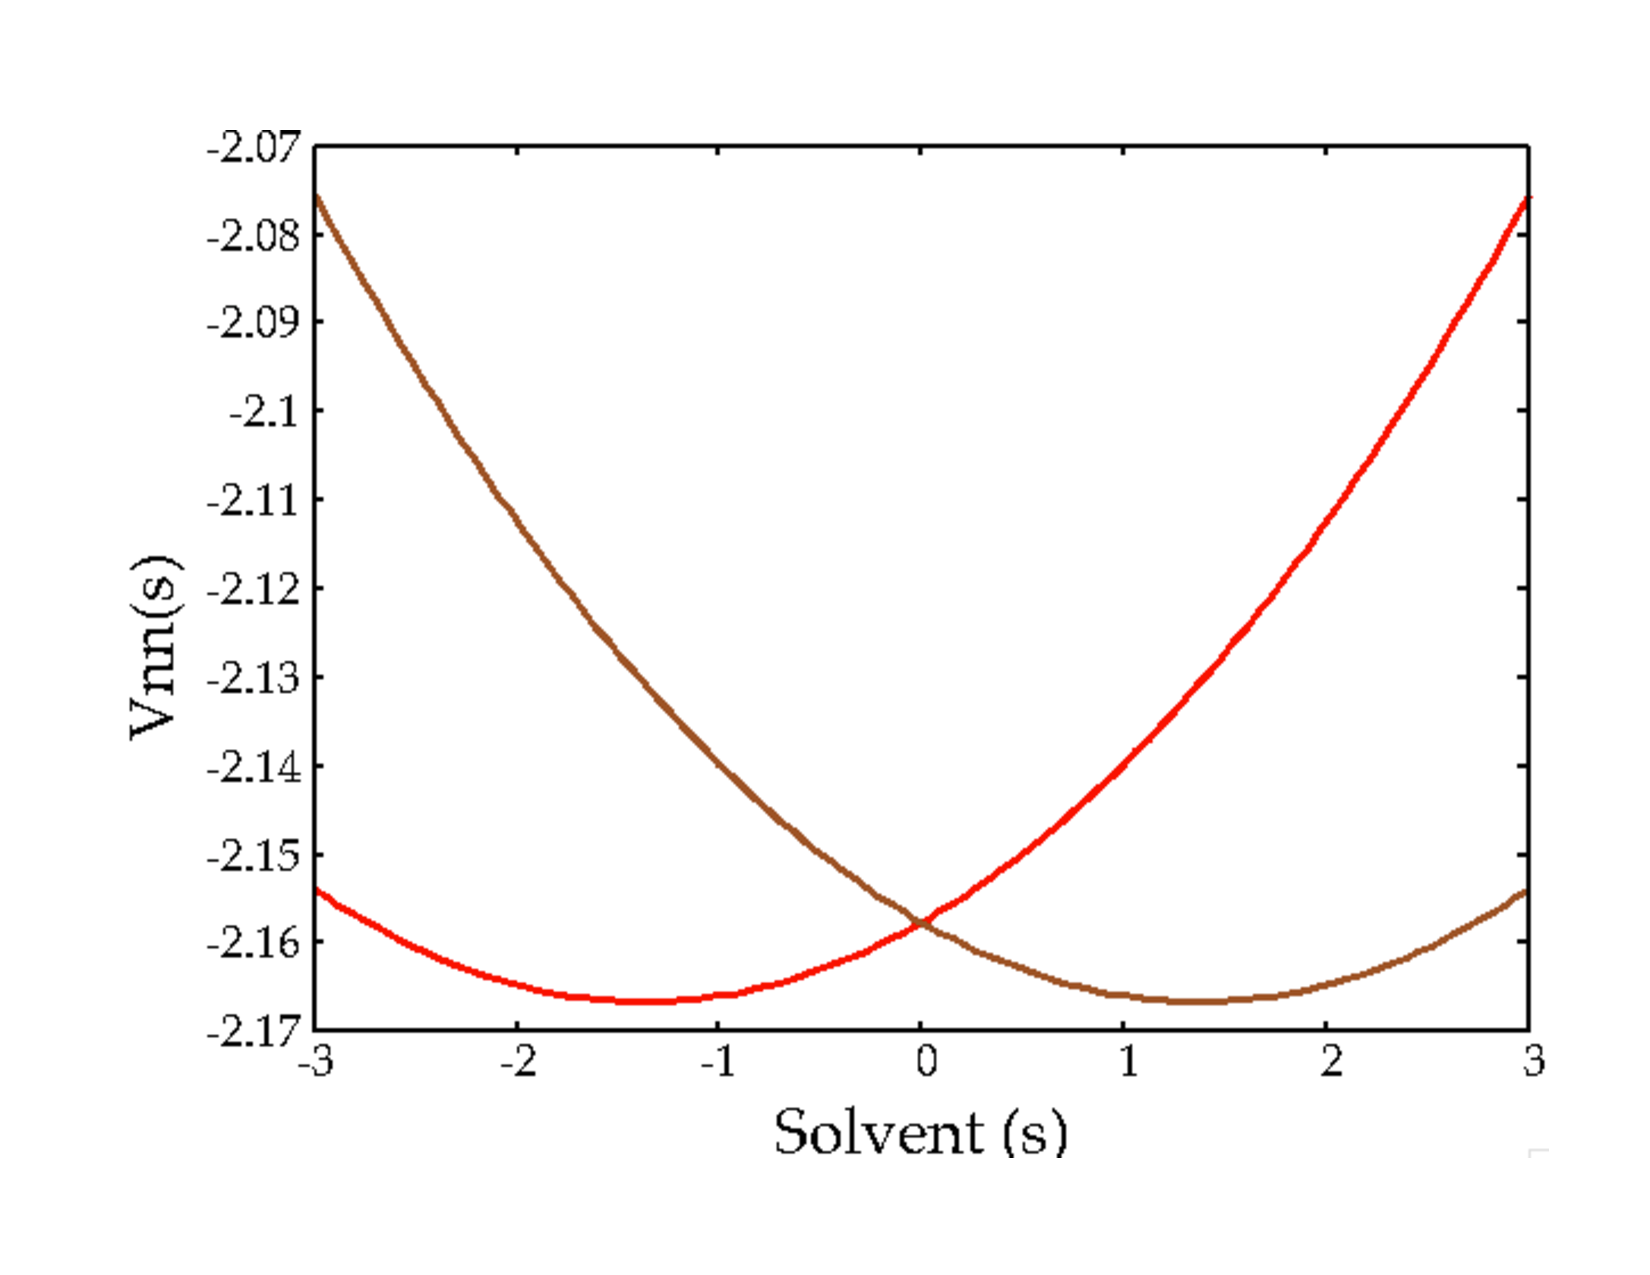
\includegraphics[scale=0.3]{etpotsym}
\vspace{-0.1in}
\caption{ Diabatic potential energy curves for ET model with state 1 in red and state 2 in brown}
\label{fig:etpotsym}
\end{figure}
Fig (2.2) shows the average energy bead convergence for the model ET system using the symmetrized QBD. Convergence is achieved with 5 beads to give an average energy of $5.36\times 10^{-3}$ with error bars on the order of $10^{-6}$. We compared these results to bead convergence achieved with the asymmetric QBD and found that at 6 beads, the symmetrized QBD generates statistics with error bars an order of magnitude smaller than the asymmetric QBD. This suggests that the symmetrized Trotter splitting of the diabatic matrix increases the stability of the statistics. This is attributed to the fact that the elements in the symmetrized diabatic matrix are symmetrically modulated by neighboring beads. 
\begin{figure}[h!]
\vspace{-0.25in}
\centering
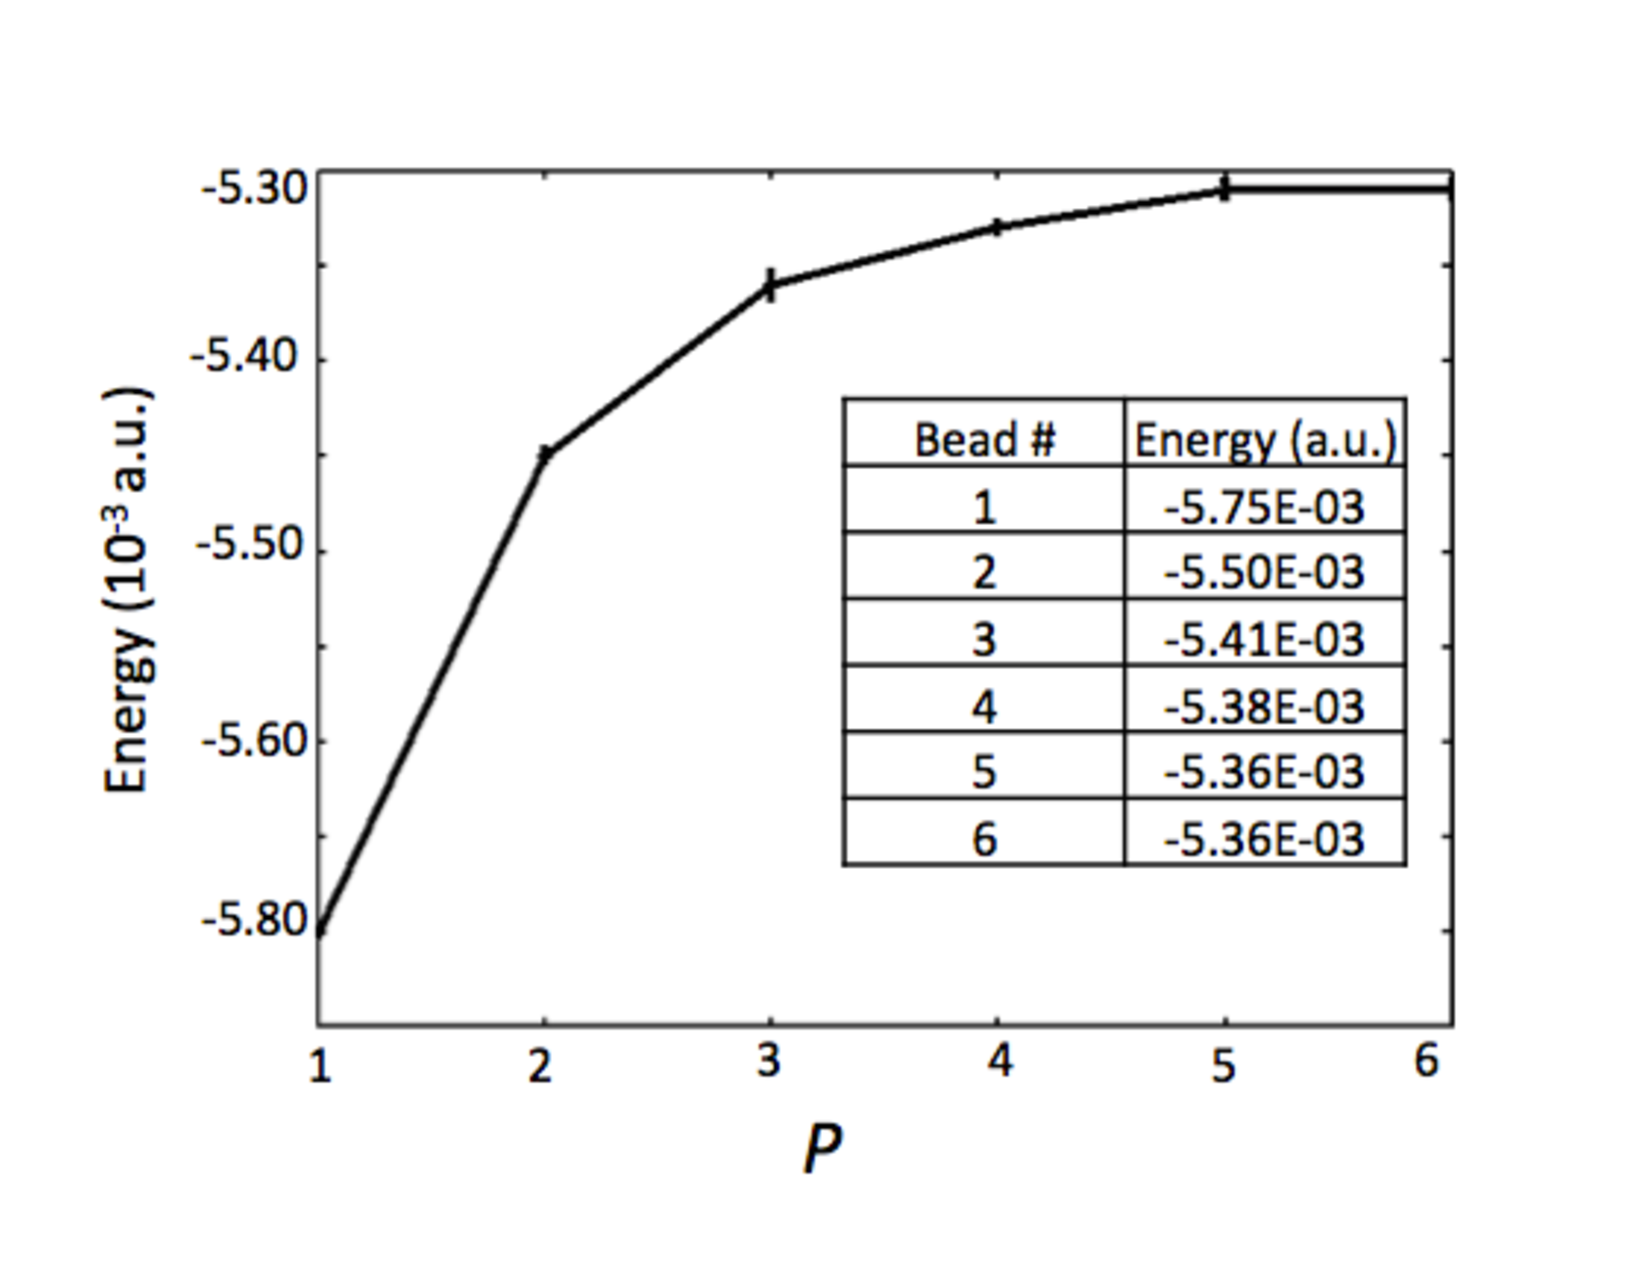
\includegraphics[scale=0.4]{etsymeconverge}
\vspace{-0.15in}
\caption{Average energy bead convergence}
\label{fig:etsymeconverge}
\end{figure}

\subsection{MV-RPMD Trajectories and Correlation Functions}
In general, thermal real-time correlation functions in the 
MV-RPMD framework are written as 
\begin{equation} 
\label{eq:tcorr}
C_{AB}(t) = \frac{\langle \textrm{sgn}(\Theta) A(\{\bf{\xi}_\alpha\}_0)
B(\{\bf{\xi}_\alpha\}_t) \rangle_{W}}{\langle \textrm{sgn}(\Theta) \rangle_W},
\end{equation} 
where $\{\bf{\xi}_\alpha\}_t$ represents the set of 
bead positions and momenta \{$\bf{R}_{\alpha},\bf{P}_{\alpha}, 
\bf{x}_{\alpha},\bf{p}_{\alpha}$\} at time $t$,
and the bead-averaged function $A(\{{\bf{\xi}}_\alpha\}_0)=
1/N \sum_\alpha A(\bf{\xi}_\alpha (0))$ and $B(\{\bf{\xi}_\alpha\}_t)$ 
is similarly defined.
The initial positions and momenta are generated from 
a standard Path Integral Monte Carlo (PIMC) simulation
that employs the sampling function, $W$. 
This corresponds to a system initially at equilibrium,  
$W = e^{-\beta_{{N}} H_{N}(\{\bf{\xi}_\alpha\}_0)}$, with 
the MV-RPMD Hamiltonian, $H_N $, defined in 
Eq. (2.39). However, this function can 
also be defined to describe an initial non-equilibrium 
distribution as discussed later on (see Section 4.4).
Real-time trajectories are generated by integrating 
equations of motion corresponding to the 
MV-RPMD Hamiltonian,
\begin{eqnarray}
\nonumber
\dot{{\bf{R}}}_{\alpha}&=& 
\frac{\partial H_P}{\partial
{\bf{P}}_{\alpha}}\;,\;
\dot{{\bf{P}}}_{\alpha}= -\frac{\partial
H_P}{\partial {\bf{R}}_{\alpha}}\\
\dot{{\bf{x}}}_{\alpha}&=&  \frac{\partial
H_P}{\partial {\bf{p}}_{\alpha}}\;,\;
\hfill \hfill \dot{{\bf{p}}}_{\alpha}=
-\frac{\partial H_P}{\partial
{\bf{x}}_{\alpha}}. 
\label{eq:eom2}
\end{eqnarray}
These trajectories preserve the QBD for a $P$-level system. Upon evaluating the derivatives in terms of $H_P$ in Eq. (2.39) we get, 
\begin{equation}
 \dot{{\bf{R}}}_{\alpha} = \frac{{\bf{P}}_{\alpha}}{M}
\end{equation}

\begin{equation}
 \dot{{\bf{P}}}_{\alpha} =-\frac{MP}{\beta^2} (2 {\bf{R}}_{\alpha}- {\bf{R}}_{\alpha+1}- {\bf{R}}_{\alpha-1})  -\bigg( \frac{\partial V_0}{\partial {\bf{R}}_{\alpha}} \bigg)  -\frac{P}{\beta \Theta} \bigg( \frac{\partial V_0}{\partial {\bf{R}}_{\alpha}} \bigg)
\end{equation}

\begin{equation}
[ \dot{{\bf{x}}}_{\alpha}]_j = \frac{2P}{\beta}[{\bf{p}}_{\alpha} ]_j  -\frac{P}{\beta \Theta} \bigg( \frac{\partial \Theta}{\partial [{\bf{p}}_{\alpha} ]_j}\bigg)
\end{equation}

\begin{equation}
[ \dot{{\bf{p}}}_{\alpha}]_j = -\frac{2P}{\beta}[{\bf{x}}_{\alpha} ]_j +\frac{P}{\beta \Theta} \bigg( \frac{\partial \Theta}{\partial [{\bf{x}}_{\alpha} ]_j}\bigg)
\end{equation}


where $[]_j$ refers to the $j^{th}$ component of the electronic variable. Again, real-time TCFs in the RPMD framework are identical to the Kubo-transformed correlation functions at time zero and the same is true for MV-RPMD TCFs. For example the Kubo-transformed nuclear position-position TCF is, 

\begin{equation}
\tilde{c}_{RR}(t) = \frac{1}{\beta Z} \int_{0}^{\beta} \textrm{tr}[e^{-(\beta -\lambda)\hat{H}}\hat{R}(0)e^{-\lambda \hat{H}} \hat{R}(t)]d\lambda
\end{equation}
and the corresponding MV-RPMD correlation function is written as, 

\begin{equation}
C_{RR}^{\textrm{MVR}} (t) =\frac{1}{Z} \int d\{ {\bf{x}}_{\alpha} \} \int d\{ {\bf{p}}_{\alpha}\} \int d\{ {\bf{R}}_{\alpha}\} \int d\{ {\bf{P}}_{\alpha}\} e^{-\beta_P H_P(\{ {\bf{x}}_{\alpha} \},\{ {\bf{x}}_{\alpha} \},\{ {\bf{x}}_{\alpha} \},\{ {\bf{x}}_{\alpha} \})} \bar{{\bf{R}}}(0)\bar{{\bf{R}}}(t)\textrm{sgn}(\Theta).
\end{equation}
\section{Summary}
In this chapter we reviewed the imaginary-time path integral discretization of the QBD which results in what is known to be the classical isomorphism between the classical statistics of a ring polymer and the exact quantum statistics of a quantum particle. We explored the basic theory of RPMD, an efficient yet approximate method that preserves the QBD and provides a consistent dynamic framework reaction dynamics. We mentioned some of the limitations of RPMD, including its inability to capture real-time quantum coherence beyond $t= \beta \hbar$, and describe multi-electron/multi-state quantum systems. We described nonadiabtatic extensions of RPMD, including MV-RPMD and nonadiabatic MF-RPMD (both developed in our group) and their applications to classes of nonadiabatic reactions. 

We then provided a derivation of an improved QBD in the MV-RPMD framework where the symmetric Trotter approximation is invoked and generated statistics for a model ET system with increased stability in convergence. We also provided the mathematical formalism required to generate approximate quantum dynamics in the MV-RPMD framework with the goal of calculating real-time TCFs. 

Given MV-RPMD's success at capturing excited state dynamics in the gas phase, it is now of interest to consider nonadiabatic multi-particle reactions in the condensed phase. Eventually we'd like to use MV-RPMD in the simulation of proton coupled electron transfer reactions. The next section will review some of the PCET model systems reported in the literature which will set the ground work for PCET simulations in the condensed phase with MV-RPMD. 


\chapter{Modeling PCET}
PCET reactions are typically described in terms of a reactant, metastable intermediate, and product species,
\begin{equation}
\textrm{D}-\textrm{H} +\textrm{A}  \quad (\textrm{D}_{e}\textrm{D}_{p})
\end{equation}
\begin{equation}
[\textrm{D}-\textrm{H}]^{+} +\textrm{A}^{-}  \quad (\textrm{D}_{e}\textrm{A}_{p})
\end{equation}
\begin{equation}
\textrm{D}^{-}+ [\textrm{H} -\textrm{A}]^{+}  \quad (\textrm{A}_{e}\textrm{D}_{e})
\end{equation}
\begin{equation}
\textrm{D} + \textrm{H}-\textrm{A}  \quad (\textrm{A}_{p}\textrm{A}_{e})
\end{equation}

Here D and A represent donor and acceptor molecules respectively, and $\textrm{D}_{e}\textrm{D}_{p}$ corresponds to both the electron and proton being on the donor, $\textrm{D}_{e}\textrm{A}_{p}$ correspond to the electron being on the donor and the proton being on the acceptor, $\textrm{A}_{e}\textrm{D}_{e}$ corresponds to the electron being on the acceptor and the proton being on the donor, and $\textrm{A}_{p}\textrm{A}_{e}$ corresponds to both the electron and the proton being on the acceptor. The reaction mechanism can be categorized as either sequential or concerted depending whether both the electron and proton transfer in a single step. In the concerted mechanism the proton and electron transfer simultaneously without the formation of metastable intermediates. In the sequential mechanism you can have either the proton transfer first, forming the metastable  $\textrm{D}_{e}\textrm{A}_{p}$ species, followed by electron transfer to form the product $\textrm{A}_{p}\textrm{A}_{e}$ species. Conversely in a sequential mechanism an electron can transfer first, forming the intermediate species $\textrm{A}_{e}\textrm{D}_{e}$, followed by proton transfer to form the product species $\textrm{A}_{p}\textrm{A}_{e}$. 

\section{Model Systems}
In this section we will review the various PCET model systems that have been reported in the literature as well as the model PCET system we develop in this study. Further, we will comment on the extent of RPMD and MV-RPMD's applicability across model systems.  
\subsection{Capped Coulomb Potentials Coupled to Proton Double Well}
The first model to consider for PCET is a co-linear system bath model ~\cite{TFM2016}, where in the position representation we have the potential energy function,
\begin{equation}
U(q_e, q_p, q_s, {\bf{Q}})= U_{sys}(q_e, q_p, q_s) + U_B(q_s, {\bf{Q}})
\end{equation}

where $U_B(q_s, {\bf{Q}})$  is the potential energy term associated with the bath coordinate, and system potential energy is, 
\begin{equation}
 U_{sys}(q_e, q_p, q_s)=U_e(q_e)+ U_p(q_p)+U_s(q_s)+U_{es}(q_{e}, q_s)+U_{ps}(q_{p}, q_{s})+U_{ep}(q_{p}, q_{e})
\end{equation}

The variables $q_e$, $q_p$, $q_s$, are scalar coordinates that describe the positions of the electron, electron, proton and solvent respectively. The vector ${\bf{Q}}$ describes the bath oscillator positions. The first term in the system potential models the interaction between the transferring electron and the donor and acceptor sites, 

\begin{equation}
   U_e(q_e)=\left\{
     \begin{array}{ll}
     a_{D}q_e^2+b_Dq_e +c_D, & r_D^{\textrm{out}} \leq q_e \leq r_D^{\textrm{in}}\\
     a_{A}q_e^2+b_Aq_e +c_A, & r_A^{\textrm{out}} \leq q_e \leq r_A^{\textrm{in}}\\
     -\mu_e\bigg[ \frac{1}{q_e-r_d}+\frac{1}{q_e-r_d}\bigg], & \textrm{otherwise}
    \end{array}\right.
    \label{eq:hs}
\end{equation}

In Eq.  (3.7) $r_D$ and $r_A$ are the positions of the electron donor and acceptor sites. This model consists of two symmetric Coulombic wells which are capped by quadratic functions to remove singularities. The second term,  $ U_p(q_p)$, is a quartic potential which models the interaction between the transferring proton and the donor and acceptor cites,

\begin{equation}
U_p(q_p)= - \frac{m_p \omega_p^2}{2} q_p^2+  \frac{m_p^2 \omega_p^4}{16V_0} q_p^4.
\end{equation}
 Here, $\omega_p$ is the proton vibrational frequency, and $V_0$ is the proton transfer barrier height. The solvent potential is defined as 
 \begin{equation}
 \frac{1}{2} m_s \omega_s^2 q_s^2
 \end{equation}
 
 where $m_s$ is the solvent mass, and $\omega_s$ is the effective frequency of the solvent coordinate. The coupling between the electron and solvent is defined as
 \begin{equation}
 U_{es}(q_{e}, q_s)=-\mu_{es} q_e q_s.
 \end{equation}
Similar the coupling between the electron and proton is defined as,
 \begin{equation}
 U_{ps}(q_{p}, q_s)=-\mu_{ep} q_p q_s.
 \end{equation}
 Interaction between the transferring electron and proton are modeled via the capped Coulombic potential
 
 \begin{equation}
   U_{ep}(q_{ep})=\left\{
     \begin{array}{ll}
       - \frac{\mu_{ep}}{q_e-q_p}, & |q_e-q_p|>R_{cut}\\
    -\frac{ \mu_e}{R_{cut}}, & \textrm{otherwise}.
    \end{array}\right.
    \label{eq:hs}
\end{equation}
The term $U_B(q_s , {\bf{Q}})$ models the dissipative bath that is coupled to the PCET reaction. The bath exhibits an ohmic spectral density $J(\omega)$ with the cutoff frequency designated by $\omega_c$. The density is defined as, 
\begin{equation}
J(\omega) = \eta \omega e^{-\omega/\omega_c},
\end{equation}
where $\eta$ is the friction coefficient. The density is discretized into $f$ oscillators with frequencies defined as,
\begin{equation}
\omega_j = - \omega_c \textrm{ln} \bigg( \frac{j - 0.5}{f} \bigg) 
\end{equation}
and the coupling constants are defined as 
\begin{equation} 
c_j = \omega_j \bigg( \frac{2 \eta M \omega_c}{f \pi} \bigg)^{1/2}.
\end{equation} 

Miller and coworkers find dynamic and equilibrium calculations to converge with $P=32$ for the proton coordinate and $P=1024$ for the electron coordinate. These bead convergence parameters depend on the mass of the quantized particle, where lighter particles require a larger number of beads. While Miller and coworkers successfully use RPMD to capture PCET rates across multiple regimes, a shortcoming is in it's treatment of electron and proton as distinguishable particles. The next model PCET system discussed moves away from treating the electron as a distinguishable particle by representing discrete electron acceptor and donor states in terms of a solvent polarization coupled to a proton double well. 
\subsection{Two electronic states coupled to Proton Double Well}
Hamiltonian for PCET
where the proton is represented in 
position space and a two-state system
describes the electron 
transfer.
The system Hamiltonian is 
\begin{equation}
\label{eq:systemham} H
=\frac{P_{s}^2}{2m_{s}}
+\frac{P_{R}^2}{2m_{R}} + V_{p}(R) +
V_{ps}(R,s) + V_{ij}(R,s). 
\end{equation}
In Eq. (3.16), $R$ is
the proton coordinate with conjugate
momentum $P_R$, and 
$V_p (R)$ is a double well potential
in the proton coordinate,
\begin{equation}
\label{eq:protpot} V_{p}(R) =
-\frac{m_R\omega_R^2}{2}R^2 +
\frac{m_R^2\omega_R^4}{16V_0}R^4 -
\lambda R^3, \end{equation}
where $m_R$ is the mass of the proton,
$\omega_R$ is the frequency, $\lambda$ is 
a measure of anharmonicity, and $V_0$
determines the height of the barrier for
proton transfer.
Further, the proton-solvent coupling is
\begin{equation}
\label{eq:solcoup} V_{ps}
    (R,s) = -\mu_1 s \tanh (\phi R),
\end{equation}  
where $\mu_1$ and $\phi$ are constants 
that can be chosen to favor either 
concerted or sequential mechanism.
The two-state diabatic potential for 
electron transfer is 
\begin{equation} 
\label{eq:diabat2}
V_{ii}(R,s) = \frac{1}{2}m_s\omega_s^2(s
- s_i)^2 +a_i \mu_2 \tanh (\phi R),
\end{equation} where $\mu_2$, $a_i$, and
$\phi$ are constants that can be tuned 
to construct models that favor either concerted or 
sequential mechanisms. Parameters for the three
models considered here are provided in 
Table 3.1
\\
\begin{table}[h!]
\vspace{-0.25in}
\centering
\begin{tabular}{| c | c | c | c |}
   \hline
 $\textrm{Parameter}^a$ & $\textrm{Model I}$  & $\textrm{Model II}$ & $\textrm{Model III}$\\
 \hline
 $m_R$   &1836.1  &1836.1 &1836.1\\
$\omega_{R} $  &0.0104  &0.0104 &0.0104\\
$V_{0}$ &0.012  &0.014 &0.012    \\
 $s_1$ &-2.13  &-2.16 &-2.13\\
 $s_2$ &2.13 &2.16 &2.13  \\
 $V_{12}$  & 0.00245 & 0.0124 & 0.00245\\
  $\mu_1$ & 0.0011 & 0.017 & -0.0011\\
 $\mu_2 \times 10^3$ & 5.84 &0.71 & 5.84\\
 $\lambda$ & 0.0 & 0.012 & 0.0\\
 \hline
\end{tabular}
\vspace{-0.15in}
\caption{Parameters (in atomic units) for the model Hamiltonians
    in Eq. 3.16}
  %  \footnotesize{$^a$ All parameters specified in atomic units}}
\label{tab:pt_params}
\end{table}

\begin{figure}[h!]
\vspace{-0.1in}
\centering
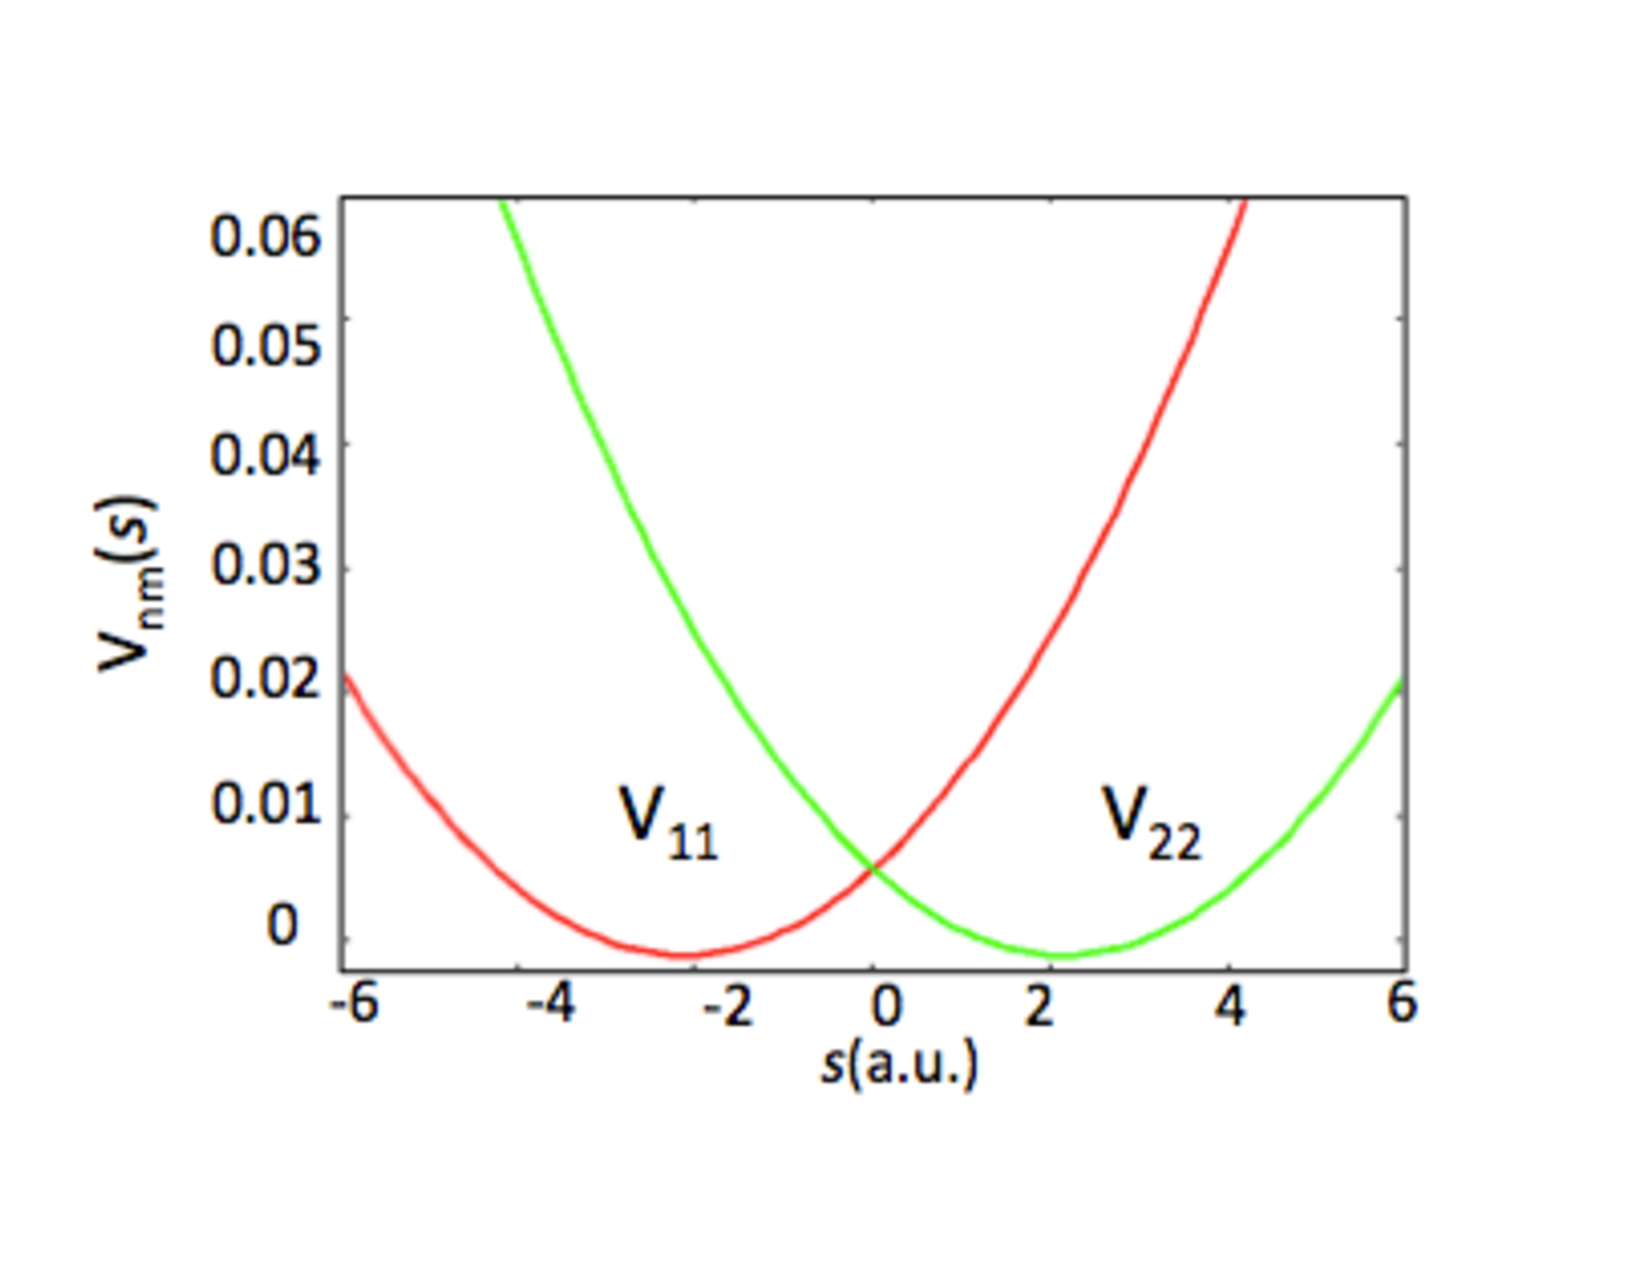
\includegraphics[scale=0.4]{twostateconc}
\vspace{-0.1in}
\caption{The diabatic states defined in terms of solvent polarization. $V_{11}(s)$ is shown in red and $V_{22}(s)$ is shown in green.}
\label{fig:twostateconc}
\end{figure}
\section{Concerted PCET}

\begin{figure}[h!]
\vspace{-0.1in}
\centering
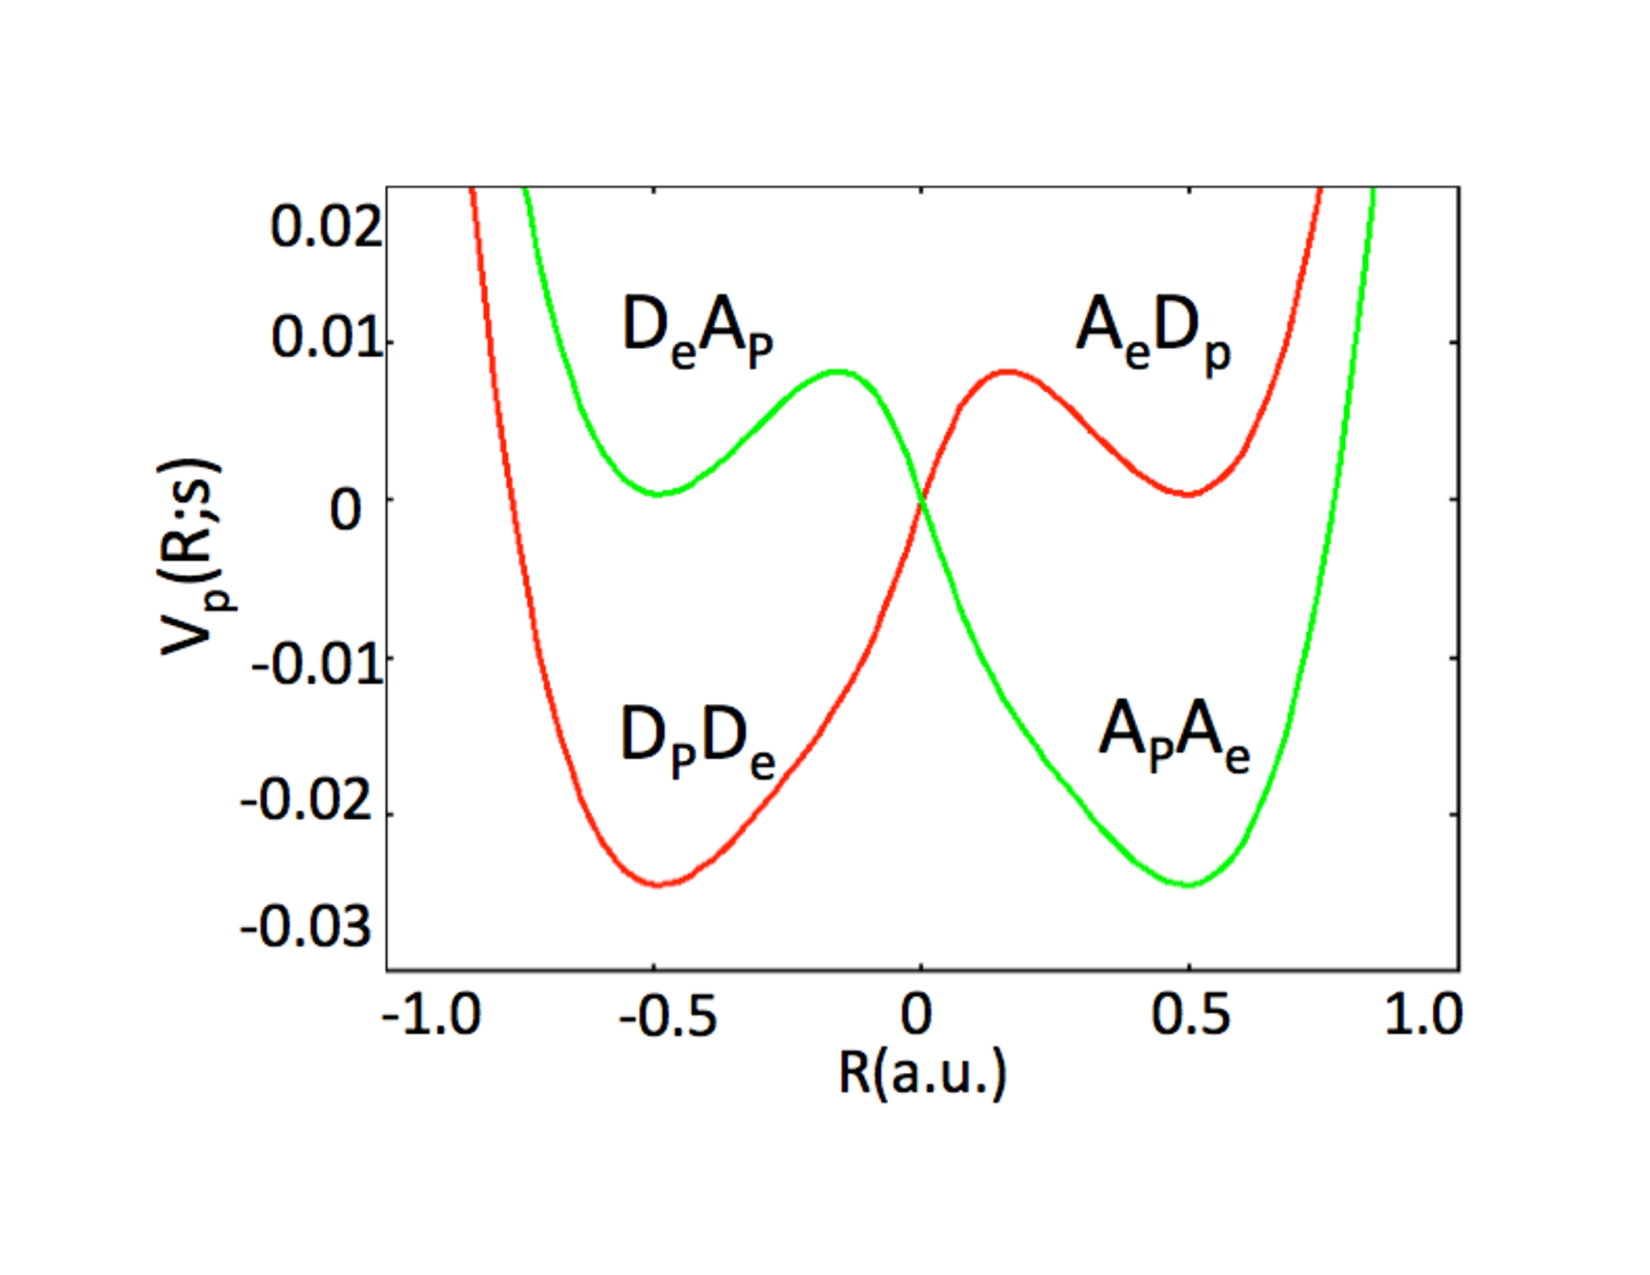
\includegraphics[scale=0.4]{proton}
\vspace{-0.1in}
\caption{The Proton double well potential coupled to solvent polarization. $V_p(R)+ V_{ps}(R;s1)$ is shown in red and $V_p(R)+ V_{ps}(R;s2)$ is shown in green.}
\label{fig:proton}
\end{figure}

In Fig.(3.2) we show state-specific proton potentials, where the red curve corresponds to the proton double well coupled to the donor electronic state and the green curve corresponds to the proton double well coupled to the acceptor electronic state. The solvent/proton coupling is described by the term $V_{ps}(R,s) = -\mu_1 s \tanh (\phi R)$. We see as we move along the red curve, the stable configuration corresponds to the proton being situated at the donor. We also see, moving from left to right along the red curve, we form a metastable configuration where the electron is situated on the donor and the proton is on the acceptor. Therefore, the process of proton transfer is modeled by moving from the stable minimum on the left (proton on donor) to the metastable configuration on the right (proton on the acceptor). Subsequently, moving from the metastable configuration on the right side on the red curve to the stable configuration in the right side of the green curve corresponds to ET. This process collectively would be described as sequential PT followed by ET. Moving from the stable configuration in the red curve on the left, to the metastable green curve on the left, followed by the stable configuration on the green curve on the right corresponds to sequential ET followed by PT. Finally, moving from the stable configuration in the red curve to the stable configuration on the green curve corresponds to concerted PCET. 


Considering the discrete electronic states ($V_{11}$ and $V_{22}$) shown in Fig. (3.1), the electron/proton coupling term $a_i \mu_2 \tanh (\phi R)$ , serves to stabilize the donor electronic state when the proton is on the donor and stabilize the electronic acceptor state when the proton is on the acceptor. When the electron is on the donor and the proton is on the acceptor, $a_i \mu_2 \tanh (\phi R)$ increases the energy of $V_{11}$ creating a metastable configuration in the electronic donor  state. Similarly, when the electron is on the acceptor and the proton is on the donor, $a_i \mu_2 \tanh (\phi R)$, increases the energy of $a_i \mu_2 \tanh (\phi R)$ creating a metastable configuration in the acceptor electronic state.  

\subsection{Equilibrium: Two State model}
In our equilibrium calculations we consider the concerted PCET system (Model I). We plot average energy as a function of bead number out to $P=16$ shown in Fig. (3.3). We run PIMC calculations out to $1\times10^{8}$ for bead calculations less than $P=12$ and use $1\times10^9$ for higher bead calculations. We find calculations with a bead number greater than 15 for this system to be numerically demanding. Given that the proton is represented with a position-space ring polymer (RP), past studies suggest we would need at least 32 beads in the proton coordinate in order to establish convergence.

\begin{figure}[h!]
\vspace{-0.25in}
\centering
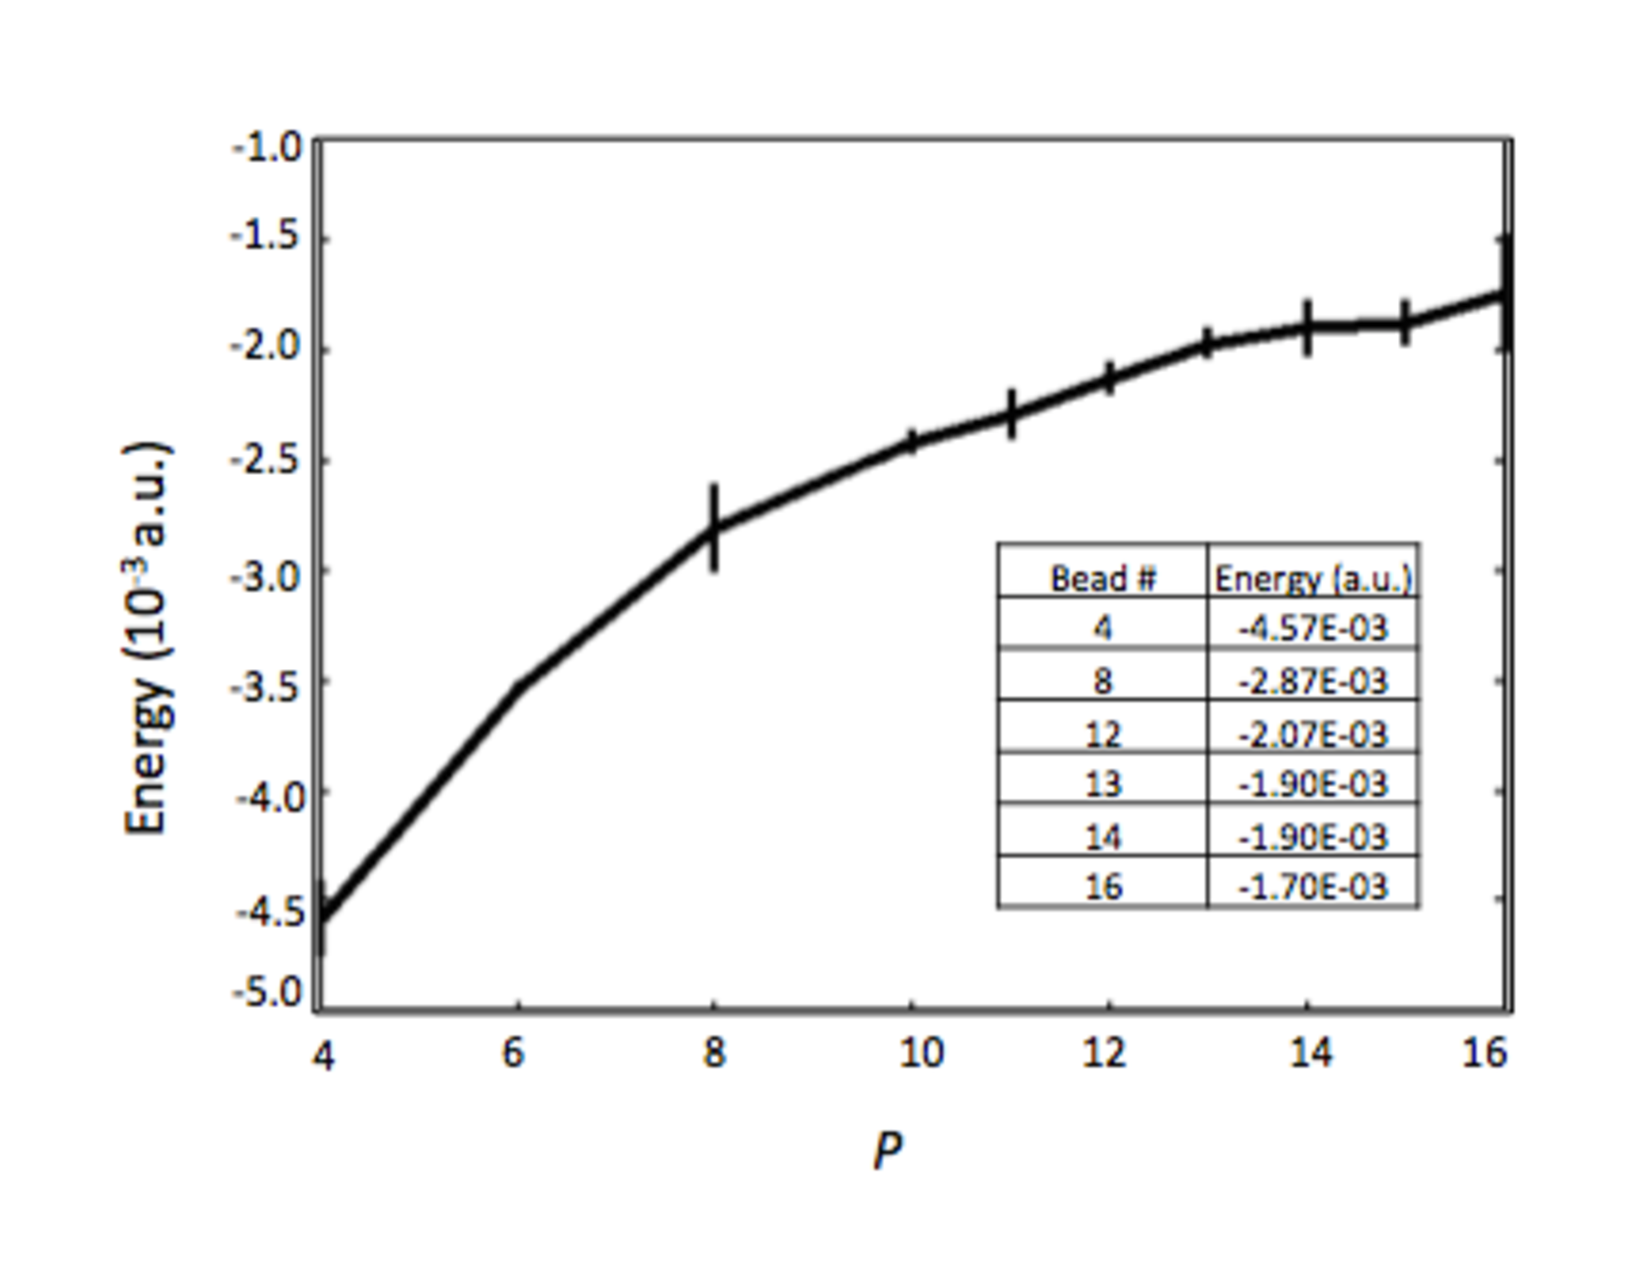
\includegraphics[scale=0.4]{etwostateconverge}
\vspace{-0.15in}
\caption{Average energy bead convergence}
\label{fig:etwostateconverge}
\end{figure}

We also calculated state-specific solvent histograms, shown in Fig. (3.4). The noise apparent in the solvent histogram is a consequence of not establishing convergence with respect to number of MC points. Despite this, we find the peaks of the solvent histograms to be situated at the local minima of the donor and acceptor electronic states.
\begin{figure}[h!]
\vspace{-0.25in}
\centering
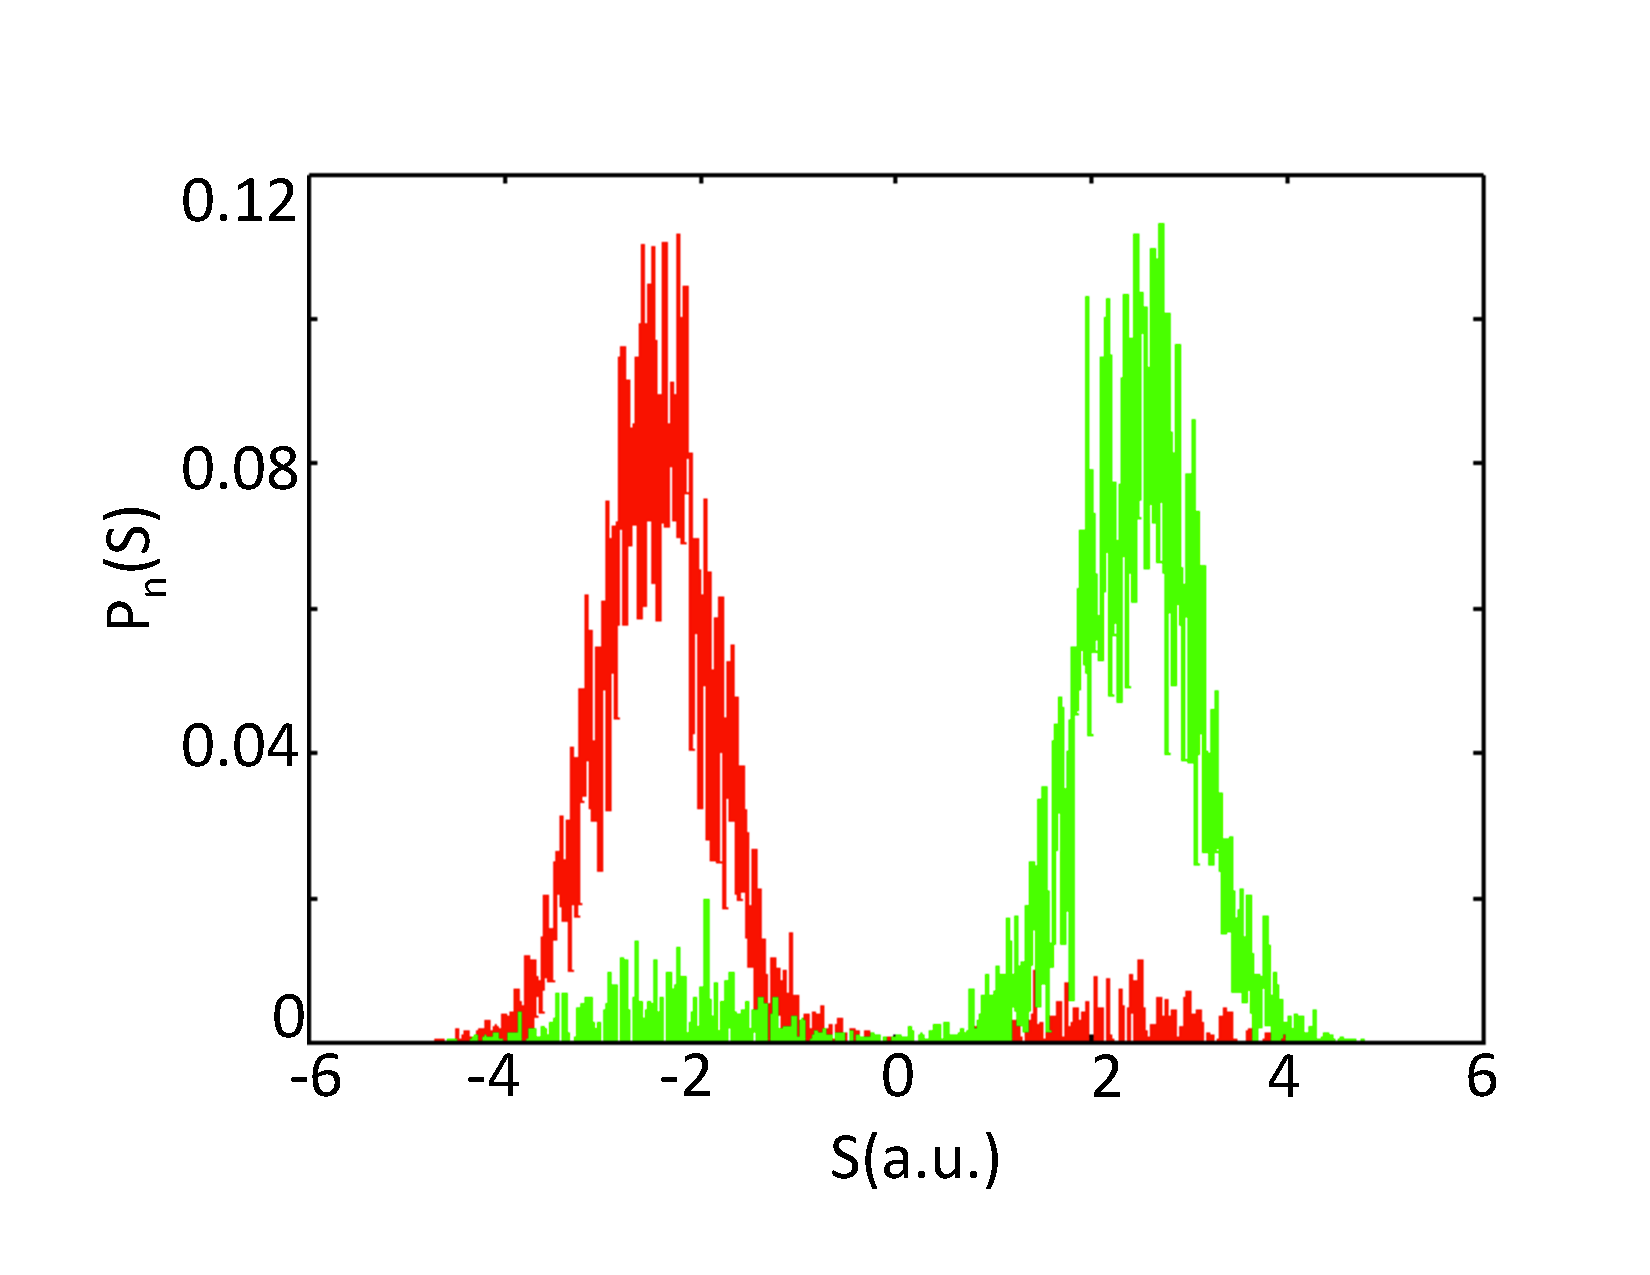
\includegraphics[scale=0.4]{solventhistfirstmodel}
\vspace{-0.15in}
\caption{State-specific solvent histogram for concerted two state coupled to proton double well model}
\label{fig:solventhistfirstmodel}
\end{figure}
We also calculated state-specific proton histograms, shown in Fig. (3.5). We find the peaks of the proton histograms to be situated at the local minima of the donor and acceptor proton configurations.
\begin{figure}[h!]
\vspace{-0.25in}
\centering
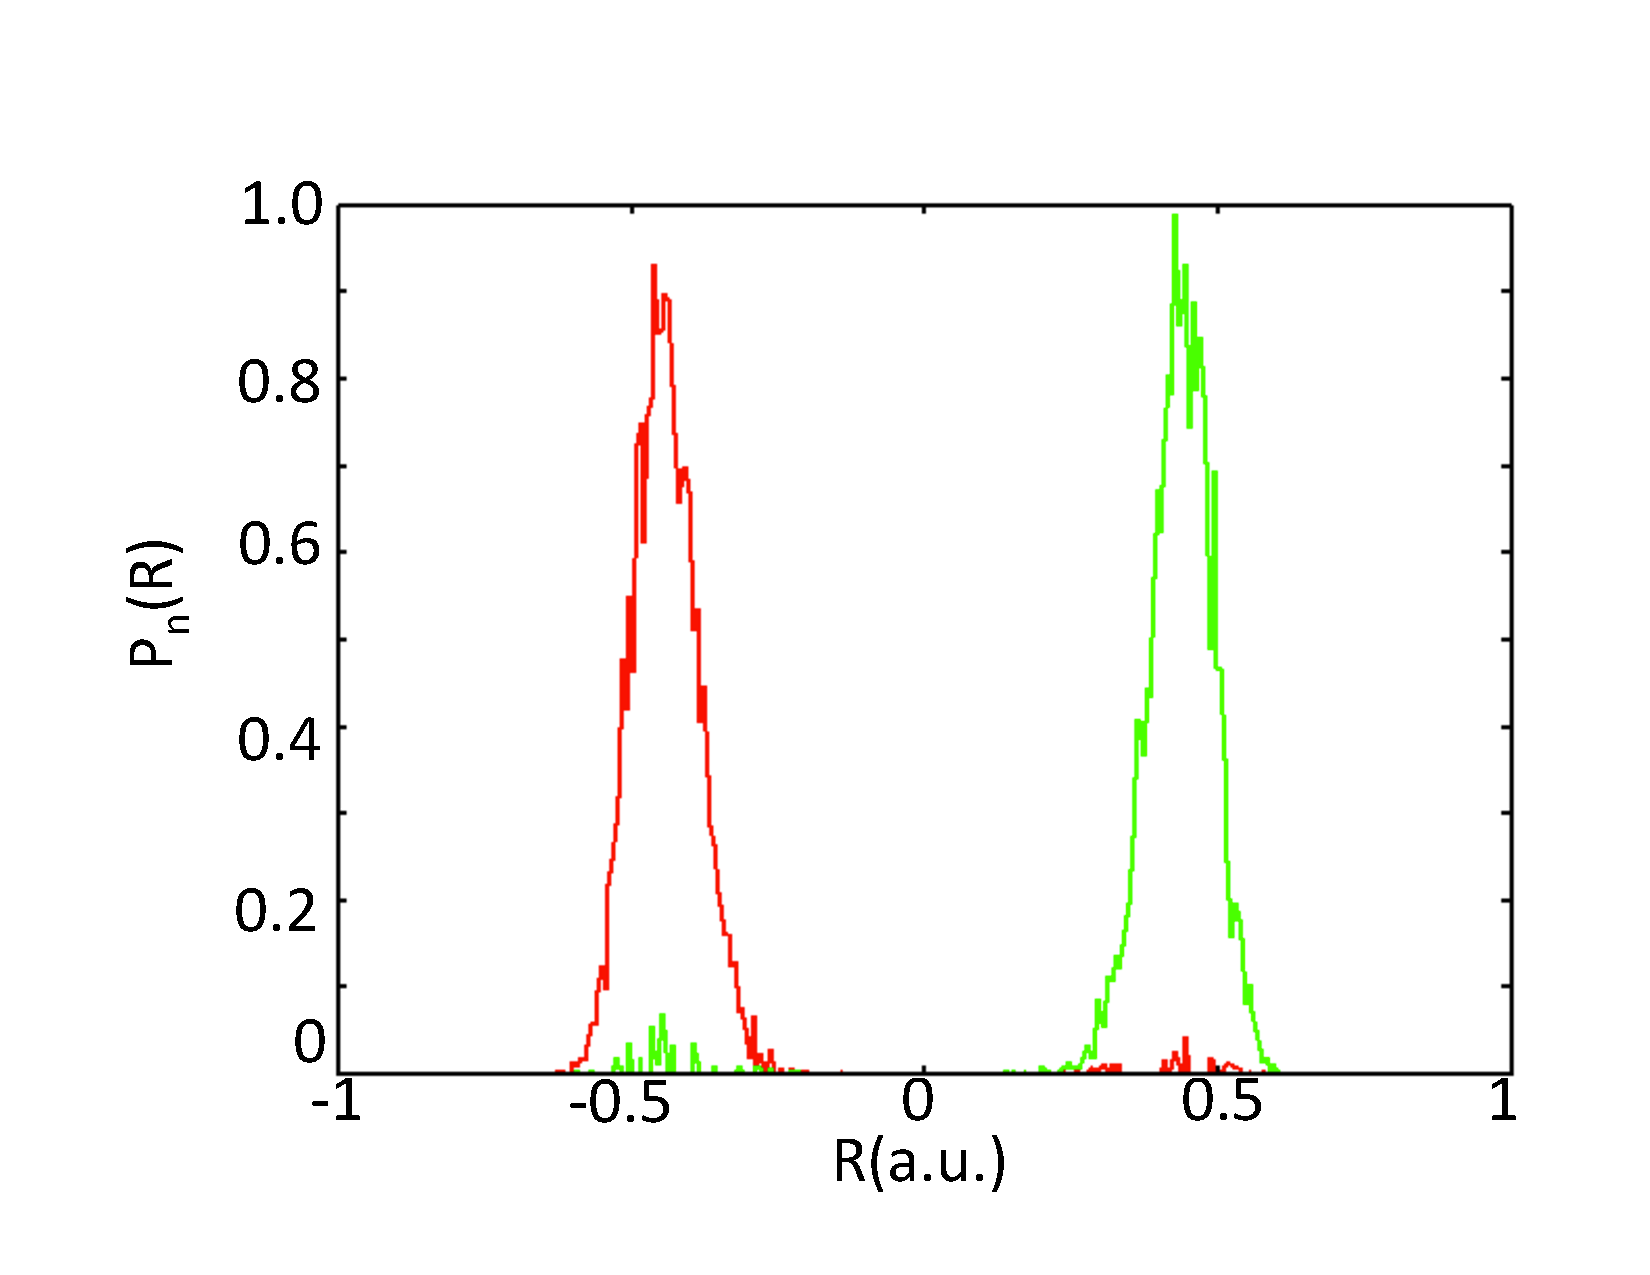
\includegraphics[scale=0.4]{protonhistfirstmodel}
\vspace{-0.15in}
\caption{State-specific proton histogram for concerted two state coupled to proton double well model}
\label{fig:protonhistfirstmodel}
\end{figure}

Since, currently we are unable to separately quantize electronic continuous variables, and proton position space variables, the $P=32$ requirement places unnecessary computational demands on converging calculations in the MV-RPMD representation since the electronic mapping variables inextricably depend on nuclear bead number. Conversely, since we are working with discrete electronic states in the MV-RPMD framework (instead of a position space RP representation) convergence with respect to the electronic coordinates depend on the ratio between coupling and temperature ($\beta\Delta$). Since we are working in the weak coupling (nonadiabatic) regime for most systems we are interested in, the burden of bead convergence would decrease in a full state space representation of our PCET system. The next section discusses how to represent the mixed state-space electron/position space proton model with four local donor/electron proton states through a quasi-diabatization procedure in concerted and sequential model systems. 


\section{Summary}
In this section we discussed two models for condensed phase PCET reported in the literature. The first is comprised of  capped Coulombic wells coupled to a proton double well potential. In the RPMD framework, Miller and coworkers represented the electronic and proton with distinct position-space ring polymers. While this works well at capturing PCET rates across multiple regimes, it treats electrons and protons as distinguishable particles and is limited to single proton/electron processes. The next model moves towards representing a broader range of PCET systems by treating the electron with discrete ET states in the MV-RPMD framework. The treatment of discrete ET states with continuous electronic conjugate variables solves the issue of treating the electron as a distinguishable particle and is generalizable to multi-electron processes. There are still two shortcomings to the mixed PCET representation. The first is that the proton is still being treated as a distinguishable particle and the model system is limited to single proton processes. Further, the position-space RP representation of the proton, imposes an unnecessary numerical demand on bead convergence since the mapping variables inextricable depend on the $P=32$ requirement for the proton coordinate. The $P=32$  bead requirement is due to the light proton mass while bead convergence with respect to electronic states depend on $\beta\Delta$. Since we work in the nonadiabatic (weak coupling) regime, bead convergence with respect to electronic mapping variables are significantly less demanding. It is then wise to consider moving away from the mixed PCET representation into a more general multi-proton/multi-electron system such as the full state-space representation of PCET. Efforts toward this goal will be the focus of the next section. 

\chapter{Simulating PCET with MV-RPMD}
\section{Diabatization: Four State electron-proton representation}

For each value of the solvent configuration 
in the range $-6 a_0 \leq s \leq 6 a_0$,
we diagonalize the system hamiltonian on 
a uniform DVR grid in the proton coordinate
with a grid range of $ -2 a_0 \leq R \leq 2
a_0$ and 100 grid points. The adiabatic
eigenstates obtained upon diagonalizing the 
system Hamiltonain are writtten as 
$\langle R;s|\epsilon_i\rangle$ where
$\epsilon_i$ is the $i^\textrm{th}$ adiabatic state
with eigenenergy $E_i$.

Further, by diagonalizing the system Hamiltonian
for a single electronic state (donor or acceptor) 
at each value of $s$, we construct localized 
proton wavefunctions, $\langle R;s | l_j \rangle$
where $l_j$ is the $j^{th} $ quasi-diabatic local
electron-proton states that can be expressed 
in terms of the adiabatic eigenstates as,
\begin{equation} \label{eq:localstate} \langle
R;s | l_j \rangle = \sum_i \int d R'
\langle R;s |\epsilon_i \rangle \langle
\epsilon_i | R';s\rangle \langle R';s | l_j
\rangle \end{equation}

Matrix elements of the Hamiltonian in
the quasi-diabatic basis can then be 
constructed using
\begin{eqnarray} \label{eq:localstate2} 
\nonumber
&& \langle
    l_j | H | l_{j^\prime}\rangle \\
\nonumber
&& = \sum_{i,i^\prime} \langle l_j| \epsilon_i\rangle
    \langle \epsilon_i | H |\epsilon_{i^\prime}\rangle
    \langle \epsilon_{i^\prime}| l_j^\prime \rangle\\
    && = \sum_{i} \langle l_j| \epsilon_i\rangle E_{i}
    \langle \epsilon_i| l_j^\prime \rangle,
\end{eqnarray}
where $E_i$ is the energy of the $i^\textrm{th}$ eigenstate
of the Hamiltonian in Eq. (3.16). 

The overlap between the reference quasi-diabatic 
wavefunction and the adiabatic state for a given 
value of the solvent coordinate, $s$, is then 
obtained by evaluating 
\begin{equation} \label{eq:overlap} \langle
\epsilon_i | l_j \rangle = \int dR \langle \epsilon_i |R \rangle
\langle R | l_j \rangle. \end{equation}

\section{PCET Model Systems} 

Previous work using RPMD for the simulation of PCET in
condensed phase model systems used a position-space 
representation to describe a single distinguishable 
electron and proton coupled to a thermal bath~\cite{TFM2013}. 
Exact quantum dynamics studies~\cite{NA2012} and 
surface hopping based simulations~\cite{SHS1997}
for similar model systems choose to employ 
a two-state representation of the electron donor
and acceptor states coupled to a position space 
proton. Here, we transform these 
model Hamiltonians to a representation where 
four localized, quasi-diabatic electron-proton 
states are coupled to a thermal bath via a solvent 
polarization coordinate. The quasi-diabatic states are labeled,
$\textrm{DD},\;\textrm{DA},\;\textrm{AD},$ and $\textrm{AA}$ 
following previous literature, where the letters 
$\textrm{D}/\textrm{A}$ indicate the donor/acceptor state of the 
particle and the first letter describes the state of the electron
while the second letter describes the state of the proton.

Following the quasi-diabatization procedure 
presented in the previous section we 
obtain a four-state system-bath PCET Hamiltonian,
\begin{eqnarray}
\label{eq:pcetham}
\nonumber
H&=&\frac{P_{s}^2}{2m_{s}} +
\sum_{X,X^\prime,Y,Y^\prime=\textrm{D}}^\textrm{A}
|XY \rangle V_{XYX^\prime Y^\prime}(s) \langle X^\prime Y^\prime|
\\
&&+\sum_{j} \frac{P_{j}^2}{2M} + 
\frac{1}{2} M\omega_{j}^{2} (Q_{j} - 
\frac{c_js}{M\omega_{j}^2})^{2}.
\end{eqnarray}
where $s$, $P_s$ and $m_s$ are the position, momentum,
and mass of the solvent polarization coordinate,
$V_{XY,X^\prime Y^\prime}(s)$ are the elements of the diabatic potential 
energy matrix where the subscripts $X/Y/X^\prime/Y^\prime=\{D,A\}$ label
the donor and acceptor states of the particles.
In Eq.~\ref{eq:pcetham}, $P_j$, $Q_j$ and $M$ are the momentum, position and mass of the $j^{th}$ bath mode,
and $c_j$ is the coupling between the solvent and 
the $j^\textrm{th}$ bath mode of frequency $\omega_j$.
The bath spectral density is Ohmic,
\begin{equation}
\label{eq:specden}
J(\omega) = \eta \omega e^{-\omega/\omega_\textrm{c}},
\end{equation}
with cut-off frequency $\omega_c=\omega_s$ 
and the dimensionless parameter $\eta/m_s\omega_s$ 
determines the coupling strength between the solvent 
and the bath modes~\cite{ACAL1983}.
The continuous spectral density is discretized into
$f$ oscillators with frequencies~\cite{ICDM2005}
\begin{equation}
\label{eq:omegaj}
\omega_j = -\omega_\textrm{c}\textrm{log} 
\bigg( \frac{ j- 0.5}{f} \bigg),
\end{equation}
and the coupling constants $c_j$ are defined as
\begin{equation}
\label{eq:bathcoup}
c_j = -\omega_j \bigg( \frac{2 \eta M \omega_\textrm{c}}{f \pi} \bigg)^{1/2},
\end{equation}
where $j=1, \dots ,f$.

The diagonal elements of the potential
energy matrix in Eq.~\ref{eq:pcetham} obtained through
our quasi-diabatization protocol are fitted to quadratic
polynomials of the form,
\begin{equation}
\label{eq:diabats}
V_{XYXY}(s)= a s^2+b s+c
\end{equation}
and the off-diagonal couplings are taken to be constants that
are independent of the solvent coordinate.
%The diabatic potential energy surface parameters for 
%all three models are provided in Appendix~\ref{app:diab_params} 
%along with the values of the couplings between diabatic states,
%$V_{XY,X^\prime Y^\prime}$.

\section{State Population Dynamics}
For the PCET model systems considered here,
the nuclear position vector, 
$\mathbf{R}_\alpha=(s_\alpha,\mathbf{Q}_\alpha)$,
includes both the 1D solvent coordinate coupled 
to the local electron-proton states and the 
positions of all the bath modes.

Here, we investigate the mechanism of thermal PCET
by initializing trajectories to a non-equilibrium 
distribution, $\rho_\textrm{neq}(0)$, corresponding 
to a particular choice of dividing surface.
We then track the electron-proton state population dynamics 
by evaluating the real-time quantum correlation function,
%system has an initial non-equilibrium 
%distribution, $\rho_\text{neq}(0)$,
\begin{equation}
\label{eq:popcorr} 
C_{P_n,h}(t)= \textrm{Tr}\left[
\rho_\textrm{neq}(0)\mathcal{P}_{n}(t)h\right],
\end{equation} 
where the heaviside function, $h$, is defined in terms of 
the solvent coordinate and allows us to separately 
ensemble average over 
trajectories moving forward (from the dividing surface 
    towards reactants) and backwards (towards products),
\begin{equation}
    h=\left\{
     \begin{array}{ll}
      h(s_t - s^\ddagger) & \textrm{forward}\\
      h(s^\ddagger-s_t) & \textrm{backward.}
    \end{array}\right.
    \label{eq:hs}
\end{equation}
%trajectories to a dividing surface 
In the MV-RPMD framework, the heaviside function in 
Eq. (4.10)%~\ref{eq:popcorr}, 
is written in terms of the solvent ring polymer 
centroid, $h~\equiv~h(\pm(\bar s_t-s^\ddagger))$, 
where $\bar s~=~1/N\sum_{\alpha=1}^N s_\alpha$.
%where $\rho_\text{neq}$ is obtained by initializing MV-RP 
The $n^\textrm{th}$ state populations at time $t$ are 
evaluated using the `Boltzmann' estimator~\cite{NA2013,NA2015},
\begin{equation}
\label{eq:boltzpop} 
\mathcal{P}_n^{\beta} =
\frac{{\bf{\Gamma}}_{nn}}{\textrm{Tr}[{\bf{\Gamma}}]},
\end{equation}
where $\mathbf{\Gamma}_{nn}$ is a 
diagonal element of the  matrix previously defined in 
Eq. (2.57) and the time-evolved positions
and momenta are obtained by integrating 
the MV-RPMD equations of motion in Eq. (~\ref{eq:eom2}).

To initialize trajectories to the dividing surface,
we define an initial non-equilibrium density operator,
$\rho_\textrm{neq}~=~\rho_\textrm{neq}^\textrm{sys}\otimes
\rho_\textrm{eq}^\textrm{bath}$ 
where the full system is divided into a relevant subsystem 
described with non-equilibrium initial conditions and the bath 
that is initially at equilibrium.
The subsystem density matrix is defined by
\begin{equation}
\rho_\textrm{neq}^\textrm{sys}=e^{-\beta H_s}
\delta(s-s^\ddagger)
\displaystyle\prod_{n=1}^K\delta
(P_n - \mathcal{P}_n^\ddagger),
    \label{eq:rsneq}
\end{equation}
where $H_s$ is the subsystem Hamiltonian given by the first line
of Eq. (4.4), $P_n$ is the population of the 
$n^\textrm{th}$ state, and the solvent position, $s^\ddag$, and 
electron-proton state populations, $\mathcal{P}_n^{\ddagger}$, 
together define the dividing surface.
%We choose the subsystem density matrix such that,
%such that $\text{Tr}[e^{-\beta H}\mathcal{P}_n]=P_n^\ddagger$,
%and $\text{Tr}[\rho_\text{neq}\hat R]=R^\ddagger$.
Ignoring the Boltzmann weights associated with each 
electronic state, we can write the corresponding constraints 
in the MV-RPMD framework as,
\begin{equation}
    \rho_\textrm{neq}^\textrm{sys}(0)=e^{-\beta H_{RP}(s)}
    \delta(\bar s_0-s^\ddag) 
    \displaystyle\prod_{n=1}^K
    \delta(\mathcal{P}_n^{\textrm{SC}}(0)-\mathcal{P}_n^\ddagger),
    \label{eq:rneq}
\end{equation}
where the nuclear ring polymer Hamiltonian 
is defined in Eq. (2.40) and $\bar s_0$ 
is the nuclear RP centroid constrained 
to its dividing surface value, $s^\ddag$.
Further, in Eq. (4.13), we use
the recently derived `semiclassical' estimator~\cite{hel16}, 

\begin{equation}
\label{eq:scpop}
\mathcal{P}_n^{\textrm{SC}}=
\frac{1}{N} \sum_{\alpha=1}^{N} 
\left[\mathcal P_n^\textrm{SC}\right]_\alpha 
= 
\frac{1}{2N} \sum_{\alpha=1}^{N} 
(\left[x_{\alpha}\right]_n^2+ \left[p_{\alpha}\right]_n^2 -1),
\end{equation}
where $\left[ \mathcal P_n^\textrm{SC} \right]_\alpha$
is the state population associated with 
the $\alpha^\textrm{th}$ bead.
We note that this population estimator was rigorously
derived in the context of MV-RPMD to yield the exact
equilibrium populations at time $t=0$~\cite{hel16}, 
and is of similar form to the original semiclassical population
function~\cite{HMWM1979,GSMT1997}. 
The present 
bead-averaged form in Eq. (4.14)%~\ref{eq:scpop} 
has also been used as an estimator in the 
Nonadiabatic-RPMD method where trajectories are initialized
to an exact equilibrium path-integral distribution and time-evolved 
under the semiclassical mapping Hamiltonian~\cite{ric2017}.
Finally, it is important to recognize that constraining electronic 
state populations via $\mathcal{P}^\textrm{SC}_n$
in the correlation function in Eq. (~\ref{eq:rneq}),
does not constrain $\mathcal{P}^\beta_n$ to the
same values at $t=0$ since the latter includes
the correct Boltzmann weights for each electronic 
state at a given nuclear configuration.
%constructed here by combining these two estimators
%is also exact at zero time.
For each model, we calculate the real-time
correlation function in Eq. (4.9) %~\ref{eq:popcorr}
by sampling the initial nuclear and electronic 
non-equilibrium distribution using Path Integral 
Monte Carlo (PIMC).
The initial electronic state population variables
should be sampled subject to the bead-average 
constraint described in Eq. (~\ref{eq:rneq}).
However, following previous work~\cite{NA2015}, 
we implement this constraint 
by setting \emph{individual} bead state populations
to the desired values at the dividing surface rather
than constraining the average,
\begin{equation}
\left[\mathcal{P}_n^\textrm{SC}\right]_\alpha = 
\mathcal{P}_n^\ddag.
    \label{eq:pop_init}
\end{equation}



\subsection{Equilibrium: Four State model}
The parameters for the concerted model are reported in the appendix. 
\begin{figure}[h!]
\vspace{-0.25in}
\centering
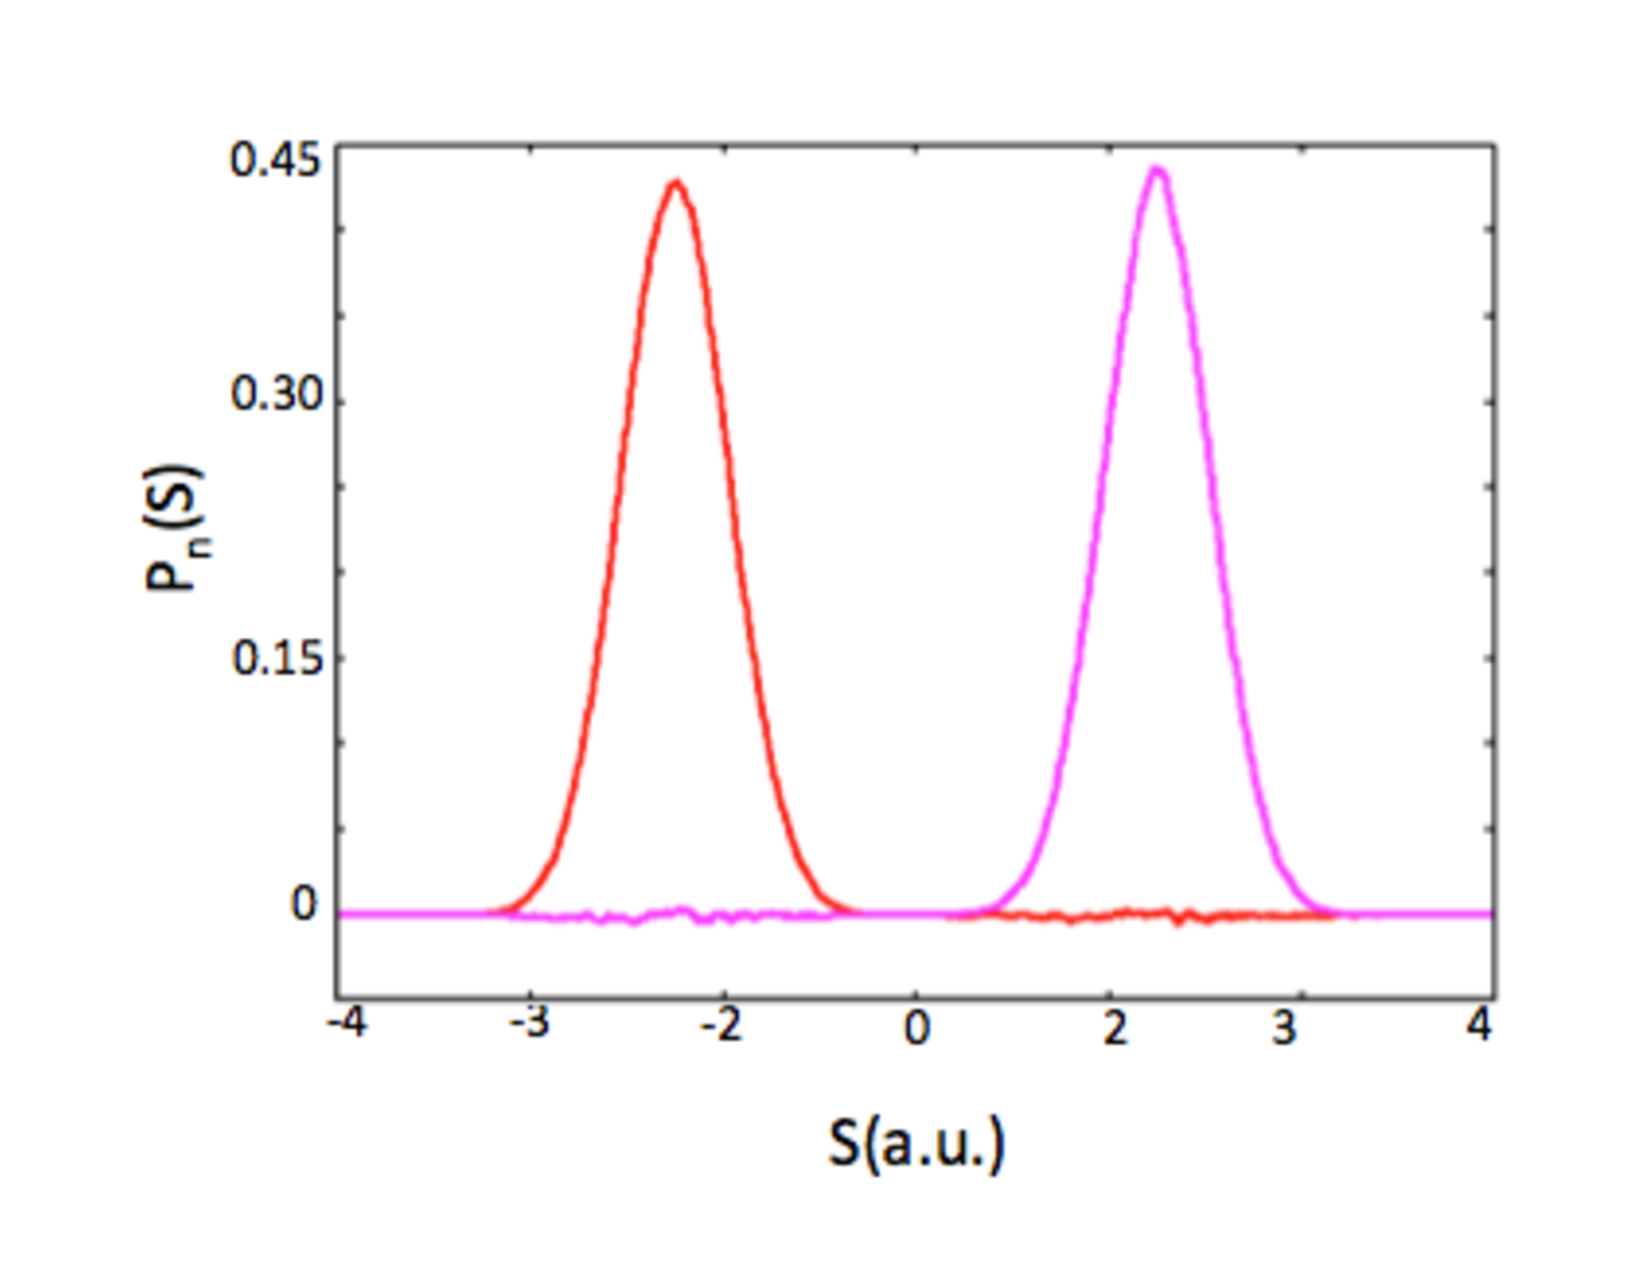
\includegraphics[scale=0.4]{solventhist1}
\vspace{-0.15in}
\caption{State-specific solvent histogram for concerted four state model}
\label{fig:solventhist1}
\end{figure}

\begin{figure}[h!]
\vspace{-0.25in}
\centering
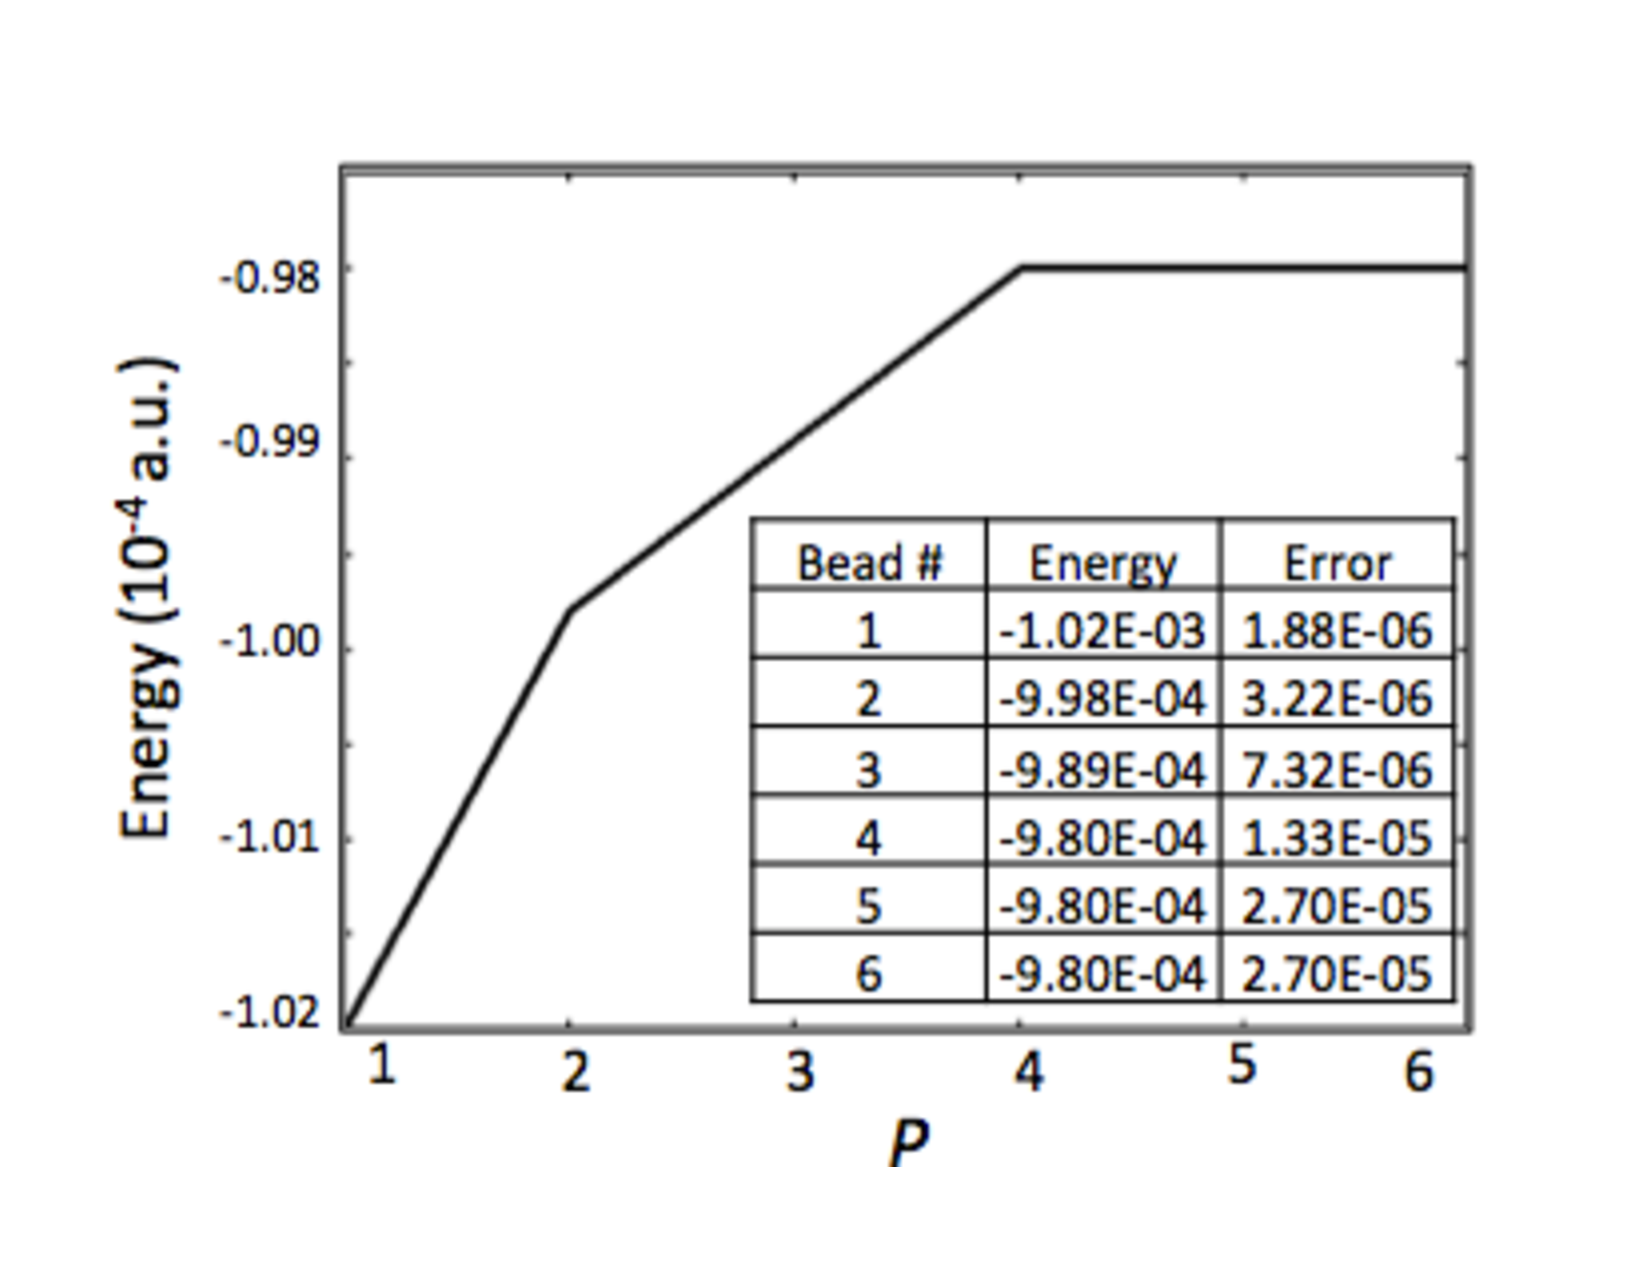
\includegraphics[scale=0.4]{econvergeconc}
\vspace{-0.15in}
\caption{Average energy bead convergence}
\label{fig:solventhist1}
\end{figure}

\subsection{Dynamics: Four State model}
The dividing surface in model I is 
chosen to be the intersection of the reactant 
($\textrm{DD}$) and product ($\textrm{AA}$) quasi-diabatic 
state potentials such that $s^\ddag=0$~a.u.
and only the $\textrm{DD}$ and $\textrm{AA}$ states are 
populated with 
$\mathcal P_{\textrm{DD}}^\ddagger~=~\mathcal P_{\textrm{AA}}^\ddag~=~0.5$ and 
$\mathcal P_{\textrm{DA}}^\ddag~=~\mathcal P_{\textrm{AD}}^\ddag~=~0$.
We sample the distribution
with a total of $5\times 10^8$ MC points 
and bead convergence is achieved with $N=10$ beads.

For model I, MV-RPMD trajectories initialized
to the dividing surface are propagated 
using a 4$^\textrm{th}$ order Adams-Bashforth-Moulton predictor
corrector integrator with a time step of size $10^{-2}$ fs.
Trajectories were integrated for a total simulation
time of $500$~fs for models I. 
The number of trajectories used to obtain the converged results
shown below were $2.5\times 10^4$.

We separate the ensemble of trajectories
into a group that moves `forward' towards product
formation (increasing values of the solvent coordinate)
and a group that moves `backward' towards the reactant state 
(decreasing values of the solvent coordinate) to obtain
the correlation function $C_{P_n,h}(t)$ 
defined in Eq. Splicing the forward and 
backward averages together at time zero, we obtain the 
population plots shown here.


\begin{figure}[h!]
\vspace{-0.15in}
\centering
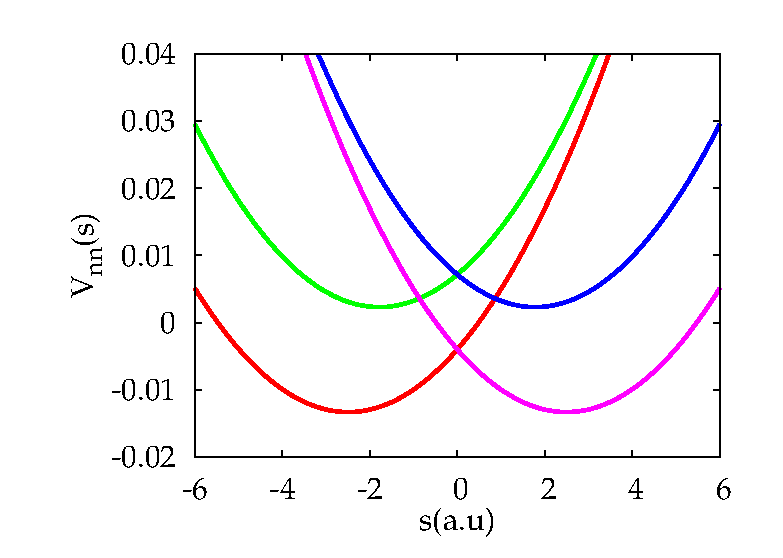
\includegraphics[scale=0.8]{concpot}
\vspace{-0.1in}
\caption{ The quasi-diabatic state potentials 
as a function of solvent coordinate are shown
for model I, with state $\textrm{DD}$ in red, 
$\textrm{DA}$ in green, $\textrm{AD}$ in blue, 
and $\textrm{AA}$ in pink.}
\label{fig:concpot}
\end{figure}
\begin{figure} [h!] 
\vspace{-0.25in}
\centering
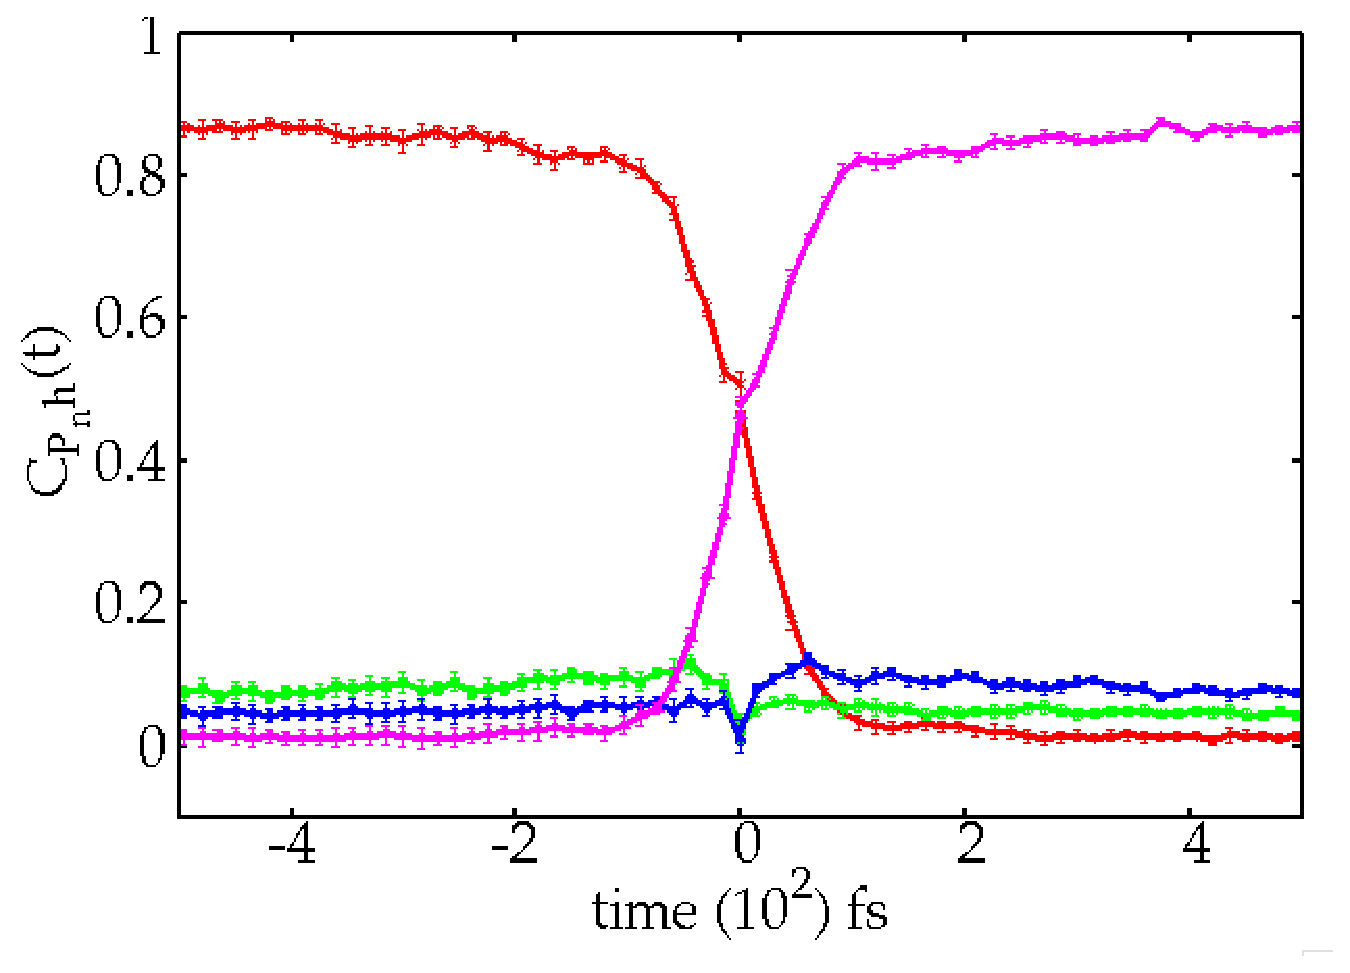
\includegraphics[scale=0.4]{pcetnew}
\vspace{-0.1in}
\caption{Population dynamics for model I (concerted), 
where population transfers directly from the 
reactant DD state (in red) to product AA state in pink. 
The intermediate AD (in blue) and DA (in green) states are
not populated during the course of the reaction.}
\vspace{-0.1in}
\label{fig:pcetpop}
\end{figure}
This indicates 
a concerted PCET mechanism where the proton and 
electron transfer simultaneously on a sub-picosecond time scale. 
The energetically unfavorable AD and DA states are not 
involved in the PCET process, but we find a 
small population in both states that decays to zero 
at long times. 

\section{Sequential PT-ET }

\begin{figure}[h!]
\vspace{-0.25in}
\centering
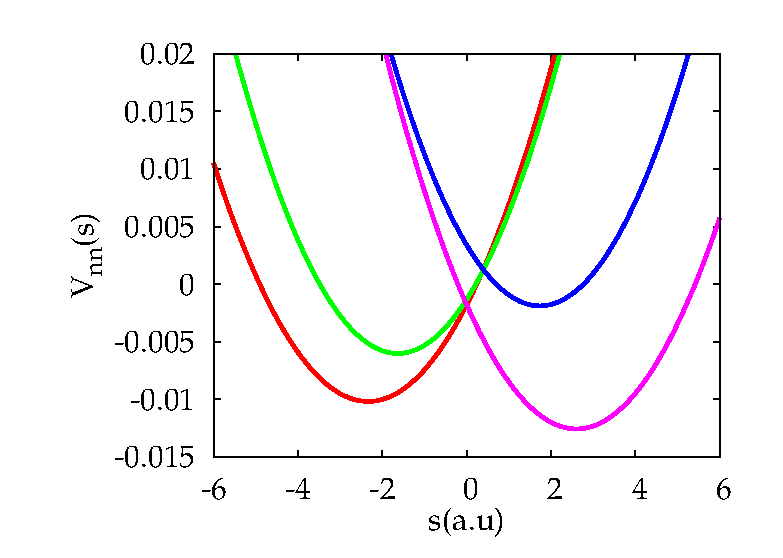
\includegraphics[scale=0.8]{ptpot}
\vspace{-0.15in}
\caption{The quasi-diabatic state potentials as a function of 
    solvent coordinate for model II with 
    state $\textrm{DD}$ in red, $\textrm{DA}$ in green, 
$\textrm{AD}$ in blue, and $\textrm{AA}$ in pink.}
\label{fig:ptpot}
\end{figure}

\begin{figure}[h!]
\vspace{-0.25in}
\centering
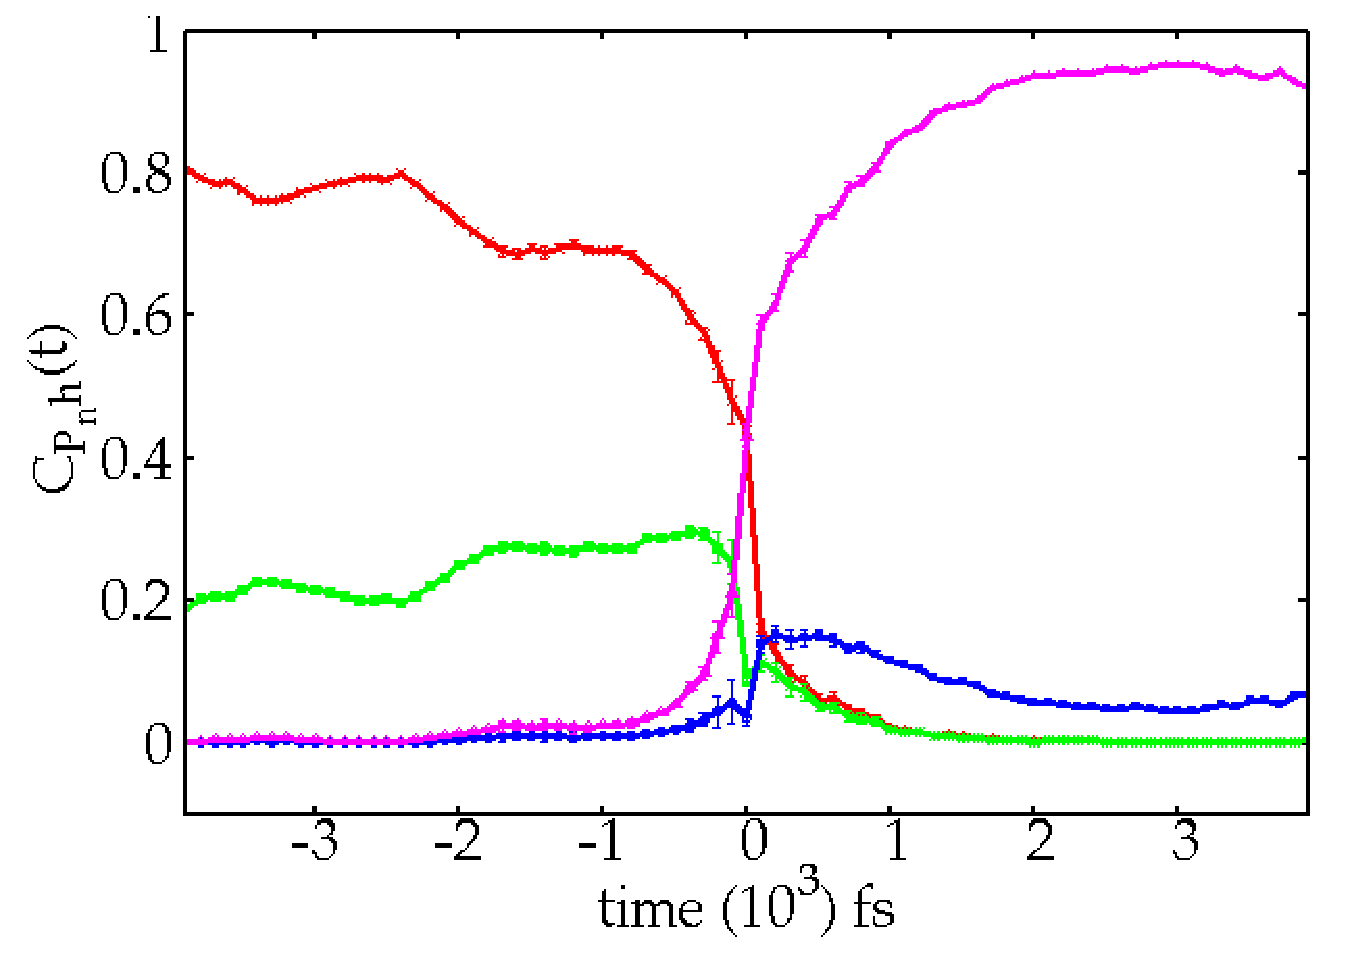
\includegraphics[scale=0.4]{PTnew}
    \vspace{-0.1in}
\caption{ 
Population dynamics for model II (sequential
PT-ET), where population first transfers from the
reactant DD state (in red) to the DA state (in green)
corresponding to proton transfer before the electron 
transfers leading to a rapid rise in the population of the
product AA state in pink.
}
\vspace{-0.3in}
\label{fig:ptpop}
\end{figure}


\subsection{Dynamics: Four State model}
The dividing surface for model II is 
chosen to be the intersection of the reactant 
($\textrm{DD}$) and product ($\textrm{AA}$) quasi-diabatic 
state potentials such that $s^\ddag=0$~a.u.
and only the $\textrm{DD}$ and $\textrm{AA}$ states are 
populated with 
$\mathcal P_{\textrm{DD}}^\ddagger~=~\mathcal P_{\textrm{AA}}^\ddag~=~0.5$ and 
$\mathcal P_{\textrm{DA}}^\ddag~=~\mathcal P_{\textrm{AD}}^\ddag~=~0$.
We sample the distribution
with a total of $5\times 10^8$ MC points 
and bead convergence is achieved with $N=10$ beads.

For model II, MV-RPMD trajectories initialized
to the dividing surface are propagated 
using a 4$^\textrm{th}$ order Adams-Bashforth-Moulton predictor
corrector integrator with a time step of size $10^{-2}$ fs.
Trajectories were integrated for a total simulation
time of  $3000$~fs. 
The number of trajectories used to obtain the converged results
shown below were $8\times 10^4$.

We separate the ensemble of trajectories
into a group that moves `forward' towards product
formation (increasing values of the solvent coordinate)
and a group that moves `backward' towards the reactant state 
(decreasing values of the solvent coordinate) to obtain
the correlation function $C_{P_n,h}(t)$ 
defined in Eq. Splicing the forward and 
backward averages together at time zero, we obtain the 
population plots shown here.



In Fig.~\ref{fig:ptpop}, we see additional 
population transfer from the DD to DA state 
on a timescale of $\approx 200$ fs preceding
the rise in the product (AA) state population. 
We also note a negligible population transfer from
the DA to AD state at short times that decays into 
thermal population in the AD state at longer times. 
These results thus suggest a sequential
mechanism for PCET where the proton transfers first, 
facilitating electron transfer.

\section{Sequential ET-PT }
\begin{figure}[h!]
   \vspace{-0.2in}
    \centering
    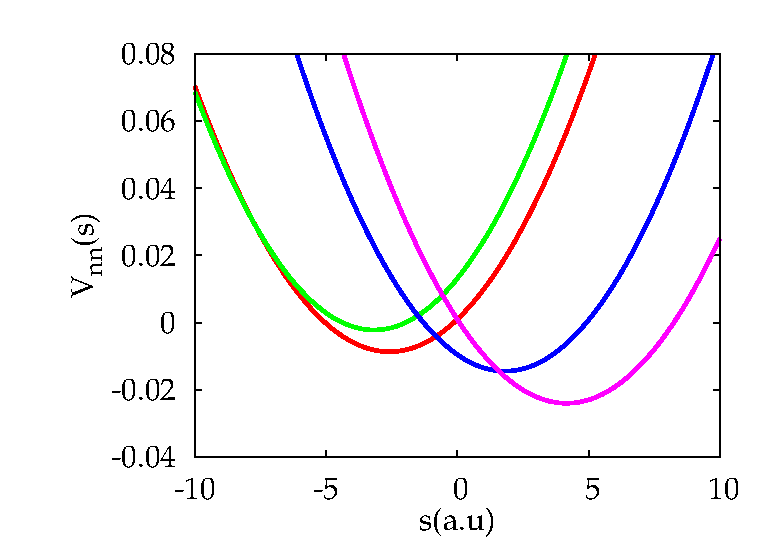
\includegraphics[scale=.8]{etpot}
\vspace{-0.15in}
\caption{ The quasi-diabatic state potentials as a function
of solvent coordinate are shown for model III, with state
DD in red, DA in green, AD in blue, and AA in pink.}
\vspace{-0.4in}
\label{fig:etpot}
\end{figure}



\quad
\subsection{Dynamics: Four State model}
The dividing surface for model III
chosen to be the intersection of the reactant 
($\textrm{DD}$) and product ($\textrm{AA}$) quasi-diabatic 
state potentials such that $s^\ddag=0$~a.u.
and only the $\textrm{DD}$ and $\textrm{AA}$ states are 
populated with 
$\mathcal P_{\textrm{DD}}^\ddagger~=~\mathcal P_{\textrm{AA}}^\ddag~=~0.5$ and 
$\mathcal P_{\textrm{DA}}^\ddag~=~\mathcal P_{\textrm{AD}}^\ddag~=~0$.
We sample the distribution
with a total of $5\times 10^8$ MC points 
and bead convergence is achieved with $N=10$ beads.

For model III, MV-RPMD trajectories initialized
to the dividing surface are propagated 
using a 4$^\textrm{th}$ order Adams-Bashforth-Moulton predictor
corrector integrator with a time step of size $10^{-2}$ fs.
Trajectories were integrated for a total simulation
time of $500$~fs. 
The number of trajectories used to obtain the converged results
shown below were $1.5\times 10^5$.

We separate the ensemble of trajectories
into a group that moves `forward' towards product
formation (increasing values of the solvent coordinate)
and a group that moves `backward' towards the reactant state 
(decreasing values of the solvent coordinate) to obtain
the correlation function $C_{P_n,h}(t)$ 
defined in Eq. Splicing the forward and 
backward averages together at time zero, we obtain the 
population plots shown here.


The diabatic potential energy surfaces
for model III is shown in Fig.~\ref{fig:etpot}
and the corresponding population dynamics in
Fig.~\ref{fig:etpop}.
We find that the system 
is initially in the reactant DD state with 
significant thermal population the DA state. 
Following the dynamics we find, however, that unlike 
model II population transfers from the reactant state 
to the AD state corresponding to electron transfer preceding 
the rise in population of the product AA state. This indicates
a sequential PCET mechanism where the electron transfers
first facilitating proton transfer. 
\begin{figure}[h!]
    \vspace{-0.2in}
    \centering
    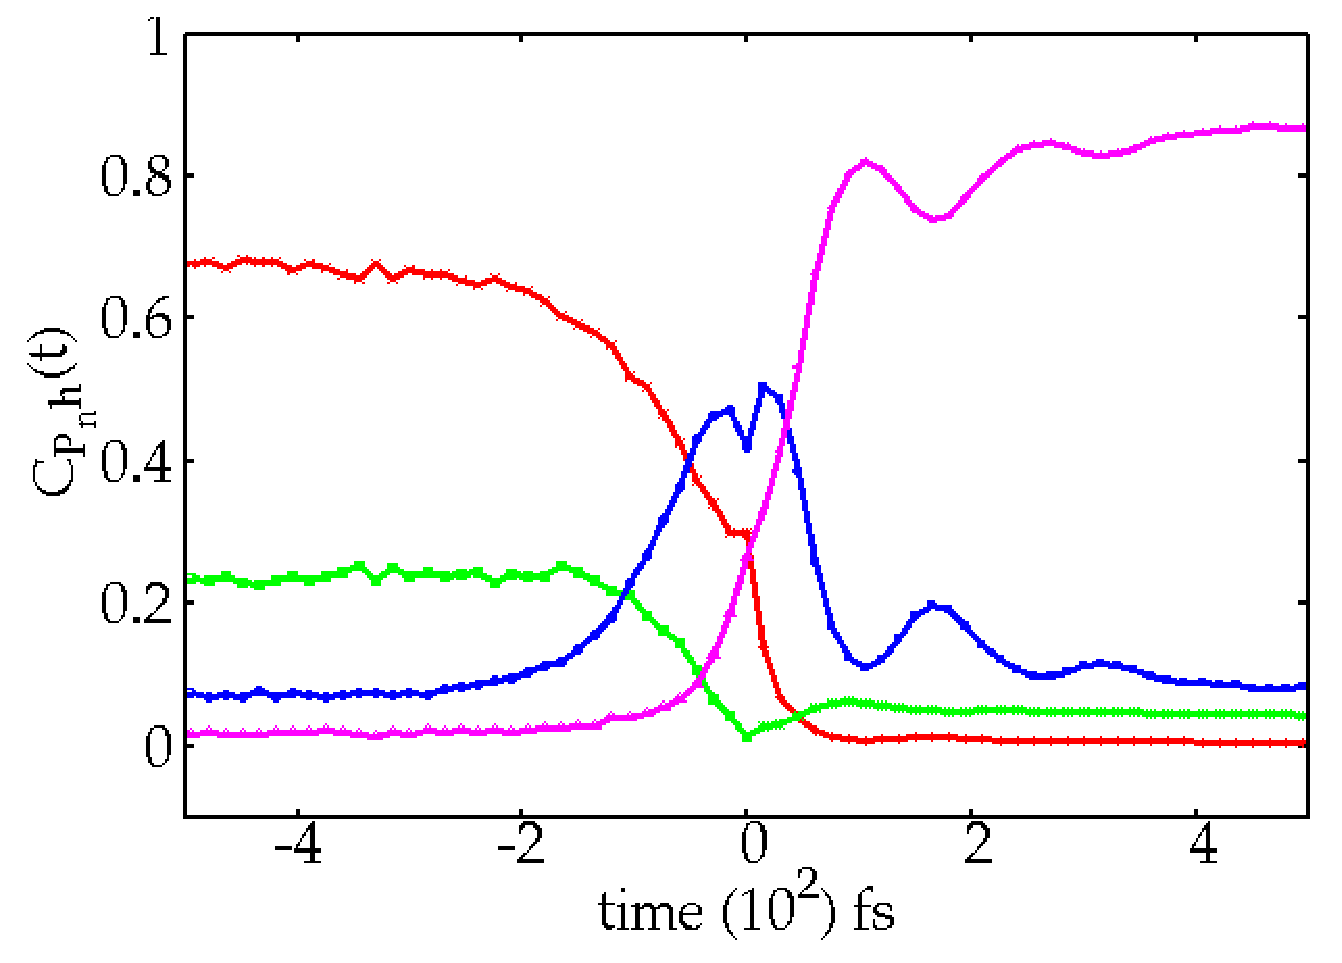
\includegraphics[scale=0.4]{ETnew}
    \vspace{-0.1in}
\caption{ 
Population dynamics for model III (sequential
ET-PT), where population first transfers from the
reactant DD state (in red) to the AD state (in blue)
corresponding to electron transfer before the proton 
transfers leading to a rapid rise in the population of the
product AA state in pink. The DA state (in green) shows 
some initial thermal population but is not populated
during the course of the reaction.
}
\vspace{-0.3in}
\label{fig:etpop}
\end{figure}


\section{Independent Dividing Surface: Sequential ET-PT }
\subsection{Dynamics: Four State model}

Finally, we use model III to 
demonstrate that the mechanism predicted by MV-RPMD 
is independent of the choice of initial dividing surface
We choose a different dividing surface with $s^\ddag=-0.8$ a.u. 
(at the intersection of the $\textrm{DD}$ and $\textrm{AD}$ states) 
and the initial electronic state populations are 
taken to be 
$\mathcal{P}_\textrm{DD}^\ddag=\mathcal{P}_\textrm{AD}^\ddag=0.5$ 
and $\mathcal{P}_\textrm{DA}^\ddag=\mathcal{P}_\textrm{AA}^\ddag=0$. 
For this simulation, trajectories were integrated for a total
time of $500$ fs and $2.5\times 10^4$ trajectories were 
employed to obtain the converged results shown here.

Despite initializing MV-RPMD trajectories to the same 
initial dividing surface for all three models, we find 
population dynamics point to three different PCET mechanisms.
Here we show that MV-RPMD simulations can yield mechanistic
insights independent of the initial choice of dividing surface
for the reactive trajectories by using a different dividing 
surface in model III. In Fig.~\ref{fig:etpop_ds} we plot the results
of this simulation where the initial dividing surface
is chosen to be at the intersection of the reactant DD 
state and the electron-transfer only AD state. We find 
the predicted mechanism is unchanged \textemdash
population transfer from the reactant state to the 
AD state first, before PCET product formation. 
\begin{figure}[h!]
\vspace{-0.1in}
\centering
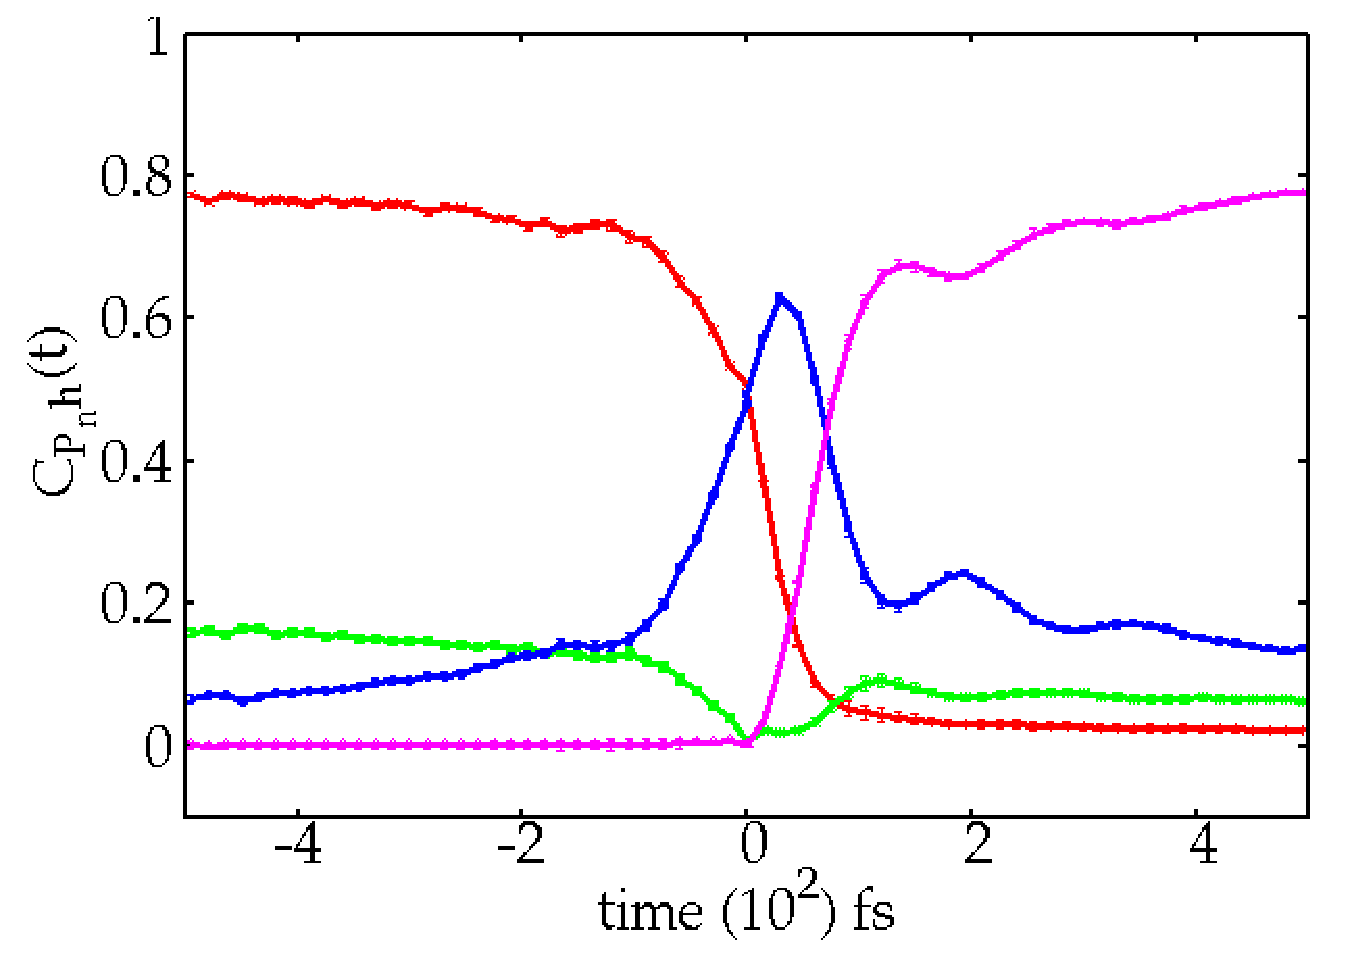
\includegraphics[scale=0.4]{indivET}
\vspace{-0.1in}
\caption{ Population dynamics for model III (sequential ET-PT), 
with reactant state in red, PT state in green, ET in blue and 
product state in pink where trajectories are initialized
to the electron transfer transition state.}
\label{fig:etpop_ds}
\end{figure}

\section{Summary}
We have extended the applicability of MV-RPMD 
to the simulation of condensed phase 
PCET using an improved formalism and 
a new population estimator to follow state
to state population transfer dynamics.
We employed a simple quasi-diabatization procedure
to build three model PCET systems where 
four local electron-proton states are coupled
to a thermal bath via a single solvent polarization 
coordinate. Following the population dynamics by 
initializing MV-RPMD trajectories to an arbitrary
dividing surface we identify the mechanism
of PCET for each of the three models and verify
the accuracy of the predicted mechanism against FGR
and Kramer's rate theory predictions. By performing a simulation with 
a different dividing surface, we were also able to clearly
establish that our MV-RPMD simulations yield mechanisms
that are independent of the initial choice of dividing surface
to which trajectories are constrained. 

The direct dynamic simulation techniques presented here 
can be readily extended to future studies of complex 
photochemical reactions and particularly photo-initiated 
PCET processes in the condensed phase. Future work in this 
direction will include deriving a systematic correction to 
the approximate MV-RPMD dynamics. In addition, we recognize
that accurately parameterizing a system-bath Hamiltonian of the 
form described in Appendix from an atomistic 
simulation remains a significant challenge.

\chapter{MV-RPMD Rate Theory}
\section{Semiclassical Instanton Theory }
There are two versions of the semiclassical instanton rate theories. The first is derived from the exact quantum flux-side correlation function. For a 1-D system, the rate expression for the first approach is ,
\begin{equation}
k_{\textrm{inst}} Z= (2\pi\hbar^3)^{-1/2} \bigg|  \frac{d^2 \bar{S}}{d\beta^2}\bigg|^{1/2}  \textrm{exp}(-\bar{S}/\hbar)
\end{equation}

where $\beta = 1/kT$, $Z$ is the reactant partition function, and $\bar{S}$ is the classical action along the "instanton" trajectory. The trajectory is a period orbit in the inverted potential with a period $\beta\hbar$. Below the "cross-over" temperature $T_c =1/k\beta_c$,  with $\beta_c = 2\pi/\hbar \omega_b$ and $\omega_b$ is the barrier frequency, one or more periodic orbits can form. 


The second, which is sometimes called the "ImF" method,  is obtained by modeling the rate of transmission through a barrier with the rate of decay of the thermal average of  shape resonances though the barrier. The method gives a rate expression with an exponent containing the action of the instanton, but a different prefactor. The rate expression is given by,

\begin{equation}
k Z_r \approx \frac{2}{\beta \hbar} \textrm{Im} R
\end{equation} 

where, 
\begin{equation}
R = \sum_k e^{-\beta (E_{{\textrm{r}} k} -i\gamma_k/2)}
\end{equation} 

Upon performing the analytic continuation of the Hamiltonian $\hat{H}$ into the complex plane, we obtain the discrete spectrum describe by the set of complex numbers $E_{{\textrm{r}} k} -i\gamma_k/2$. Deriving the instanton theory involves  a combination of steepest descent and analytic continuation applied to the exact expression for $Z_r$.

The first approach is typically preferred as it is more mathematical rigorous, but in the "ImF" approach the connection of instanton theory to RPMD becomes apparent. The following sections will give a brief review of both methods. 
\section{Miller-Schwartz-Tromp Flux-side TCF}
We start our derivation of the flux-side rate expression by considering the collinear reaction $ \textrm{A}+\textrm{BC} \to  \textrm{AB}+  \textrm{C}$, where the initial arrangement $ \textrm{A}+\textrm{BC}$ is denoted by "$a$" and the final arrangement is  denoted by "$b$". 
\begin{figure}[h!]
\vspace{-0.1in}
\centering
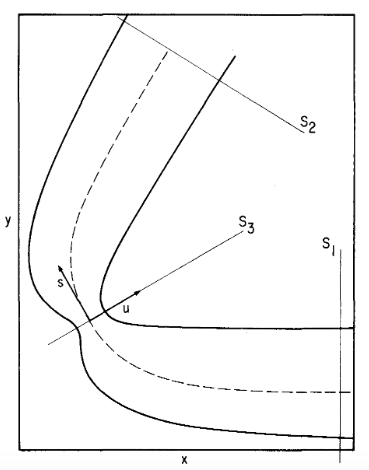
\includegraphics[scale=0.5]{fluxsurface}
\vspace{-0.1in}
\caption{Figure reprinted by permission of author ~\cite{MILLER1974}. Sketch of collinear potential energy surface for$ \textrm{A}+\textrm{BC} \to  \textrm{AB}+  \textrm{C}$.}
\label{fig:fluxsurface}
\end{figure}
The rate can be expressed as the sum over Boltzmann average of initial vibrational states and translational energy~\cite{MILLER1974,TROMP1983}, 

\begin{equation}
k_{a\to b} = (2\pi \mu kT)^{(-1/2)} Q_{BC}^{-1} \sum_{\eta_a,\eta_b} \int_0^{\infty} dE_1 e^{-\beta (E_1 + \epsilon_{\eta_a})} |S_{\eta_a, \eta_b} (E_1)|^2
\end{equation}

where $\beta= 1/kT$, $\mu$ is the reduced mass for the initial arrangement "a", $\eta_a$ and $\eta_b$ are the vibrational quantum numbers of BC and AB respectively, $E_1$ is the initial translational energy, and $  |S_{\eta_a, \eta_b} (E_1)|^2$ is the $S$ scattering matrix for the reactive process. The vibrational partition function of BC is, 

\begin{equation}
Q_{BC} = \sum_{\eta_a} e^{-\beta \epsilon_{\eta_a}}
\end{equation}

where $\epsilon_{\eta_a}$ are the vibrational energy levels of BC. In order to recast Eq. (5.4) into a more convenient form, we can introduce the notion of flux through a surface ~\cite{LSCHIFF1968}. In Figure 5.1, $x$ and $y$ are mass weighted or skewed reaction coordinates that diagonalize the kinetic energy: $x= R(\mu/M)^{1/2}$, $y= r(m/M)^{1/2}$. $R$ and $r$ are the transitional and vibrational coordinates, respectively and $\mu$ and $m$ are the reduced masses [($m$=BC/(B+C), $\mu$= A(B+C)/(A+B+C)].  $M$ is an arbitrary mass, with a corresponding classical kinetic energy $\frac{1}{2} M (\dot{x}^2 + \dot{y}^2)^2$ and $s$ and $u$ in the figure are linear combinations of $x$ and $y$ which diagonalize the potential energy at the saddle point. $\textrm{S}_1$, $\textrm{S}_2$, and $\textrm{S}_3$ correspond to 1D cuts through the 2D surface which are define by lines. Consider the first surface, $\textrm{S}_1$, defined by $R_0 -R=0$, where $R_0$ is an asymptotically large value of the coordinate $R$. The flux through $\textrm{S}_1$ in terms of the wave function $\Psi(r,R)$ is, 

\begin{equation}
-\textrm{Re} \int_{\infty}^{\infty} dr \Psi(r,R)^{*} \frac{\hbar}{i\mu}\frac{\partial}{\partial R} \Psi(r,R)| R=R_0.
\end{equation}


Here, "Re" denotes "the real part of", and a positive flux is associated with decreasing $R$, such that flux is chosen to be in the direction of the reaction. The asymptotic form of the scattering solution to the Schr$\ddot{\textrm{o}}$dinger, $(H-E)\Psi_{P_1,\eta_{a}}=0$, with $E=P_1^2/2\mu$ is, 

\begin{equation}
\Psi_{P_1, \eta_a}(r,R) \approx - \frac{\textrm{exp}(-ik_{\eta_a}R) }{(2\pi \hbar)^{1/2}} \phi_{\eta_a}(r) + \sum_{\eta_a^{'}}\frac{\textrm{exp}(-ik_{\eta_a^{'}}R) }{(2\pi \hbar)^{1/2}} \phi_{\eta_a^{'}}(r) \bigg(\frac{v_{\eta_a}}{v_{\eta_a}^{'}} \bigg) S_{\eta_a, \eta_a^{'}}(E_1)
\end{equation}

where $E_1=P_1^2/2\mu$ is the initial kinetic energy, $k_n =[2\mu(E-\epsilon_n)]^{1/2}/\hbar$ is the wave number which, and $v_n= \hbar k_n/\mu$ is the asymptotic velocity channel. This corresponds to an incident vibrational state $\eta_{a}$. The velocity channel is a normalization for the translational function, which also correspond to delta function normalization on the momentum scale. 
We can then express the flux in terms of the scattering wave function,

\begin{equation}
-\textrm{Re} \int_{\infty}^{\infty} dr \Psi_{P_1, \eta_a}(r,R)^{*} \frac{\hbar}{i\mu}\frac{\partial}{\partial R} \Psi_{P_1, \eta_a}(r,R)= 
v_{\eta_a} (2 \pi \hbar)^{-1} \bigg[ 1- \sum_{\eta_a^{'}} |S_{\eta_a, \eta_a^{'}}(E_1)|^2 \bigg]. 
\end{equation}

In the asymptotic region of "b", which is the product region, $y= r(m/M)^{1/2}$ is large, which corresponds to large value of the vibrational coordinate of AB. In the region of "b",  $\Psi_{P_1,\eta_a}$, since it corresponds to an incident wave in arrangement "a",  has only outgoing waves such that, 

\begin{equation}
\Psi_{P_1, \eta_a}(r,R_b) \approx  \sum_{\eta_b}\frac{\textrm{exp}(-ik_{\eta_b}R_b) }{(2\pi \hbar)^{1/2}} \phi_{\eta_b}(r_b) \bigg(\frac{v_{\eta_a}}{v_{\eta_b}} \bigg) S_{\eta_a, \eta_b}(E_1)
\end{equation}

where $R_b$ and $r_b$ are the translational and vibrational coordinates of AB and C respectively. The surface $\textrm{S}_2$ is defined by $R_0-R_b$ and the flux through  $\textrm{S}_2$ is, 
\begin{equation}
v_{\eta_a} (2\pi \hbar)^{-1} \sum_{\eta_a} |S_{\eta_b, \eta_a}(E_1)|^2.
\end{equation}

Because of unitarity, 
\begin{equation}
1= \sum_{\eta_a^{'}} |S_{\eta_a^{'}, \eta_a}(E_1)|^2 + \sum_{\eta_b} |S_{\eta_b, \eta_a}(E_1)|^2 
\end{equation}

we see that the flux through $\textrm{S}_1$, and $\textrm{S}_2$ are equivalent. Further the flux through any closed surface is zero which follows from the continuity equation~\cite{LSCHIFF1968},

\begin{equation}
\textrm{Re} \oint d{\bf{S}} \cdot \Psi^{*} \frac{\hbar}{i\mu} \nabla \Psi = 0. 
\end{equation}

Since $\textrm{S}_1$, and $\textrm{S}_2$  can be made into a closed surface by joining the segments at infinity, the flux through $\textrm{S}_1$, and $\textrm{S}_2$ must be equal. Writing the flux integral as a volume rather than a surface integral, we can define a surface $f(r,R) =0$, where $f(r,R)<0$ corresponds to reactant region of configuration space and $f(r,R)>0$ corresponds to the product region of configuration space. The flux through this surface written as a volume integral is, 
\begin{equation}
\textrm{Re} \int d {\bf{q}} \delta ( f({\bf{q}})) \Psi^{*}({\bf{q}}) \frac{\partial f({\bf{q}})}{\partial {\bf{q}}} \cdot {\bf{v}} \Psi ({\bf{q}}) \equiv \textrm{Re} \langle \Psi | F |\Psi \rangle
\end{equation}

where ${\bf{q}} =(r,R)$, and the components of the velocity operator are $v_k = (\hbar/im_k)(\partial/\partial q_k)$, $k=1,2$ and the flux operator is, 

\begin{equation}
F=\delta ( f({\bf{q}})) \frac{\partial f({\bf{q}})}{\partial {\bf{q}}} \cdot {\bf{v}}
\end{equation}

Now we can see that the scattering matrix can be expressed interns of the real part of the Flux operator in the basis of scattering states, 
\begin{equation}
(2\pi\hbar)^{-1} \sum_{\eta_b}|S_{\eta_b, \eta_a}(E_1)|^2 = v_{\eta_a}^{-1} \textrm{Re} \langle \Psi_{P_1, \eta_a}|F| \Psi_{P_1, \eta_a} \rangle. 
\end{equation}

We can then write the expression for the rate as, 

\begin{equation}
k_{a\to b} = Q_{a}^{-1}\sum_{\eta_a} \int_{0}^{\infty} dE_1 \textrm{exp}[-\beta(E_1 +\epsilon_{\eta_a})] v_{\eta_a}^{-1} \langle \Psi_{P_1, \eta_a}|F| \Psi_{P_1, \eta_a} \rangle
\end{equation}

where we take the real part of the right hand side of Eq. (5.16). We also should point of that the flux is independent of the choice of surface that divides reactant and product, since the flux through any closed surface is the same. Since 

\begin{equation}
e^{-\beta H} \Psi_{P_1, \eta_a} = \textrm{exp} [-\beta ( E_1+ \epsilon_{\eta_a})] \Psi_{P_1, \eta_a}
\end{equation}

and, 

\begin{equation}
E_1 =P_1^2/2\mu
\end{equation}

\begin{equation}
dE_1 =P_1/\mu dP_1 = v_{\eta_a} dP_1
\end{equation}
we can rewrite Eq. (5.16) as , 

\begin{equation}
k_{a\to b} = Q_{a}^{-1}\sum_{\eta_a} \int_{-\infty}^{0} dP_1 \ \langle \Psi_{P_1, \eta_a}|F e^{-\beta H} | \Psi_{P_1, \eta_a} \rangle
\end{equation}

where $P_1 = -(2\mu E_1)^{1/2}$. We can rewrite the integral over all momenta, negative and positive, by inserting a projection operator $\mathcal{P}$ defined by, 
\begin{equation}
     \begin{array}{ll}
      \mathcal{P}\Psi= \Psi& P_1<0\\
      \mathcal{P}\Psi= 0 &P_1>0
    \end{array}
    %\right.
    \label{eq:hs}
\end{equation}

then Eq. can be written as 
\begin{equation}
k_{a\to b} = Q_{a}^{-1}\sum_{\eta_a} \int_{-\infty}^{\infty} dP_1 \ \langle \Psi_{P_1, \eta_a}|F e^{-\beta H}\mathcal{P} | \Psi_{P_1, \eta_a} \rangle
\end{equation}

which can be rewritten in terms of the quantum mechanical trace, 
\begin{equation}
k = \frac{1}{Q_a}\textrm{tr}[ \hat{F}e^{-\beta \hat{H}} \mathcal{P}]
\end{equation}


and since  $\hat{F}$ and  $\mathcal{P}$ commute we can write the well known formally exact rate expression as ~\cite{MILLER1974,TROMP1983}, 
\begin{equation}
k = \frac{1}{Q_a}\textrm{tr}[e^{-\beta \hat{H}} \hat{F} \mathcal{P}]
\end{equation}
 where  $\hat{F}$ is the flux operator defined by,
 \begin{equation}
 \hat{F}=\delta (s)\frac{p}{m}
 \end{equation}
  where $s$ and $p$ are the reaction coordinate and momenta respectively
 the hamiltonian is, 
 \begin{equation}
 H= \frac{p^2}{2m} + V(s)
 \end{equation}

The projection operator,  $\mathcal{P}$, is defined in terms of the heaviside in the conjugate momenta,
\begin{equation}
\mathcal{P}=\lim_{t \to \infty} e^{i \hat{H} t/\hbar}h(p)e^{-i \hat{H} t/\hbar}
\end{equation}
where the heaviside function projects onto all states that have positive momentum in the infinite future ($t\to +\infty$). The reaction coordinate direction is defined from  $s\to -\infty$ to  $s\to +\infty$. 

Noting that the projection operator, $\mathcal{P}$, is defined in terms of the eigenstates of $\hat{H}$ it's clear that $[\hat{H}, \mathcal{P}]=0$. We can then rewrite Eq 5.1 in a more symmetrical form as, 

\begin{equation}
k = \frac{1}{Z}\textrm{tr}[\hat{F}e^{-\beta \hat{H}/2}  \mathcal{P} e^{-\beta \hat{H}/2} ]
\end{equation}
 and with $\mathcal{P}$ given by Eq 5.4 we can write,
 
 \begin{equation}
k = \lim_{t \to \infty}\frac{1}{Z}\textrm{tr}[\hat{F}e^{-\beta \hat{H}/2} e^{i \hat{H} t/\hbar}h(p)e^{-i \hat{H} t/\hbar} e^{-\beta \hat{H}/2} ]
\end{equation}


\section{RPMD Rate Theory}
It is perhaps not surprising that, since there is an established connection between RPMD and quantum transition state theory, RPMD has successfully been used in the calculation of reaction rates. RPMD's accuracy and efficiency allows for approximate quantum mechanical rate calculations that help inform how certain degrees of freedom within a reactive system contribute to the speed of a reaction. This is promising as we seek to better understand quantum mechanical properties of large scale systems and how knowledge of these properties may inform the design novel materials for a variety of technologies. 
In 2004 Craig and Manolopolous showed that RPMD can be used to calculate approximate Kubo-transformed flux-side correlation functions of the form ~\cite{MANO2005}, 

\begin{equation}
\tilde{C}_{fs}(t)= \frac{1}{\beta} \int_{0}^{\beta} \textrm{tr}[ e^{-(\beta - \lambda)\hat{H}} \hat{f}(0) e^{-\lambda \hat{H}} e^{+i \hat{H}t/\hbar} \hat{h}e^{-i \hat{H}t/\hbar} ]d\lambda
\end{equation}

 where $\hat{h} = h[s( {\bf{q}})]$ is a step function that projects onto the product side of the transition state dividing surface at $s({\bf{q}})=0$ and 
 
 \begin{equation}
 \hat{F} = \frac{i}{h} [ \hat{H}, \hat{h}]
 \end{equation}
 
 is the reactive flux operator.  The reaction rate coefficient can then be written as 
 
 \begin{equation}
 k = \frac{1}{Z_r} \lim_{t\to \infty} \tilde{C}_{fs}(t)
 \end{equation}
 
 where $Z_r$ is the reactant partition function. Since the side operator, $\hat{h}$ is configurational, and the flux operator $\hat{F}$ is not, the RPMD method cannot be applied directly to the Kubo-transformed flux-side correlation function. One remedy is noting that $\hat{F}$ is the Heisenberg derivative of the side operator. We can then calculate the flux-side correlation function equivalently as, 
 
 \begin{equation}
 \tilde{C}_{fs}(t) = -\frac{d}{dt} \tilde{C}_{ss}(t),
 \end{equation}
 
 where $\tilde{C}_{ss}(t)$ is a Kubo-transformed side-side correlation function,
 
 \begin{equation}
\tilde{C}_{ss}(t)= \frac{1}{\beta} \int_{0}^{\beta} \textrm{tr}[ e^{-(\beta - \lambda)\hat{H}} \hat{h}(0) e^{-\lambda \hat{H}} e^{+i \hat{H}t/\hbar} \hat{h}e^{-i \hat{H}t/\hbar} ]d\lambda
\end{equation}
 
 Since both operators in $\tilde{C}_{ss}(t)$ are configurational, RPMD can be applied and the corresponding approximation to $\tilde{C}_{fs}(t)$ can be obtained upon differentiation $\tilde{C}_{ss}(t)$. 
 
Still, there are a few issues to consider in the RPMD approximation to the Kubo-transformed flux-side correlation function. First, the operator $\hat{h}$ is a nonlinear functions of ${\hat{\bf{q}}}$. As mentioned earlier in the discussion on the features of RPMD, RPMD autocorrelation functions involving nonlinear operators having a leading error term $\mathcal{O}(t^4)$. This is particularly problematic  since we need to calculate the long-time limit of the flux-side correlation function in order to obtain a rate constant, and the method is expected to degrade with time ~\cite{MANO2006}. More worry, the Kubo-transformed flux-side correlation function has a divergent first derivative due to the integral over $\lambda$. 
 This divergence can be avoided, in an exact calculation, by alternatively using the Miller, Schwartz, and Tromp ~\cite{TROMP1983} expression for the flux-side correlation, 
 \begin{equation}
\tilde{C}_{fs}(t)= \textrm{tr}[ e^{-\beta\hat{H}/2} \hat{F}(0) e^{-\beta\hat{H}/2} e^{+i \hat{H}t/\hbar} \hat{h}e^{-i \hat{H}t/\hbar} ]
\end{equation}
 which has the same long-time limit as $\tilde{C}_{fs}(t)$ and therefore gives the same reaction rate when substituted into Eq. (6.3). We will note that this is still unsatisfactory since RPMD is an approximation and is limited to Kubo-transformed correlation functions. Nevertheless, RPMD proves to be an accurate approximation to the exact Kubo-transformed flux-side correlation function for standard models of chemical reactions, including a quartic double well coupled to a bath of harmonic oscillators ~\cite{MANO2005}. In fact the RPMD approximation of the Kubo-transformed flux-side correlation function has been shown to give comparable accuracy to the classical Wigner model ~\cite{MILLER1998,MILLER1998-2} and centroid molecular dynamics (CMD) ~\cite{VOTH2001}.
 
We will now discuss how to express Eq. (6.5) in terms of an RPMD TCF.
Consider an $d$-dimensional system described by the following Hamiltonian,

\begin{equation}
H({\bf{p}},{\bf{q}}) = \sum_{i=1}^{d} \frac{p_i^2}{2m_i} + V(q_1, \dots q_d)
\end{equation}
where we define $s$ is the reaction coordinate and the value of the reaction coordinate at the dividing sure that divided reactant and product is $s(q_1, \dots q_d)=0$ and $s>0$ corresponds to the products. The RPMD approximation to the Kubo-transformed side-side correlation function in Eq. (6.5)  for a multidimensional harmonic ring polymer  is~\cite{CHANDLER1981}, 

\begin{equation} 
\tilde{C}_{ss}(t) = \frac{1}{(2\pi \hbar)^N} \int d{\bf{P}}_0  \int d{\bf{Q}}_0 e^{-\beta_n H_n({\bf{P}}_0,{\bf{Q}}_0)} h_n({\bf{Q}}_0)h_n({\bf{Q}}_t)
\end{equation}

where $n$ is the number of ring-polymer beads, $\beta_n = \beta/n$, and $N=nd$. The Hamiltonian is, 

\begin{equation}
H_n({\bf{P}}_0,{\bf{Q}}_0)= \sum_{i=1}^d \sum_{j=1}^n \bigg[ \frac{P_{i,j}}{2m_i} + \frac{1}{2} m_i \omega_i ( Q_{i,j} - Q_{i, (j-1)})^2\bigg] \\
+ \sum_{j=1}^{n} V(Q_{1,j}, \dots, Q_{f,j}),
\end{equation}

and the flux-side TCF in the RPMD representation can be written as 

\begin{equation} 
\tilde{C}_{fs}(t) \approx \frac{1}{(2\pi \hbar)^N} \int d{\bf{P}}_0  \int d{\bf{Q}}_0 e^{-\beta_n H_n({\bf{P}}_0,{\bf{Q}}_0)} \delta ({\bf{Q}}_0)v_s({\bf{P}}_0,{\bf{Q}}_0)h_n({\bf{Q}}_t)
\end{equation}

where the rate can approximated by, 

 \begin{equation}
 k \approx \frac{1}{Z_r} \lim_{t\to \infty} \frac{1}{(2\pi \hbar)^N} \int d{\bf{P}}_0  \int d{\bf{Q}}_0 e^{-\beta_n H_n({\bf{P}}_0,{\bf{Q}}_0)} \delta ({\bf{Q}}_0)v_s({\bf{P}}_0,{\bf{Q}}_0)h_n({\bf{Q}}_t).
 \end{equation}
 


\section{ImF and RPMD}
The connection of RPMD and semiclassical instant theory arises from the application of the steepest decent approximation and analytic continuation of the ring polymer expression for the partition function. We begin by locating the saddle point on the ring polymer potential surface in the ring polymer hamiltonian, 
\begin{equation}
U_{RP}(R) =  \sum_{\alpha=1}^P V(R_{\alpha}) + \frac{mP^2}{2\beta^2\hbar^2}\sum_{\alpha=1}^P (R_{\alpha} -R_{\alpha+1})^2
\end{equation}
The stationary points of $U_{RP}$ satisfy,
\begin{equation}
V^{'}(R_{\alpha}) = m\frac{R_{\alpha+1} - 2 R_{\alpha} + R_{\alpha-1}}{(\beta_P \hbar)^2}
\end{equation}
which have the trivial solution 
\begin{equation}
R_{\alpha} = R^{\dagger}, \quad \alpha =  1, \dots , P
\end{equation}
These solutions correspond to all the normal modes of the ring polymer being zero with the exception of the centroid mode $\bar{R}_0$. The centroid mode is located at the barrier maximum $R^{\dagger}$. The normal modes $Q$ of a free ring polymer with $P$ beads correspond to the eigenstates of a $P$-member cyclic Huckel system. For an even number of beads the normal modes are given by, 

\begin{equation}
Q_0 = \frac{1}{P} \sum_{\alpha=1}^P R_{\alpha},
\end{equation}

\begin{equation}
Q_k = \bigg(\frac{2}{P} \bigg)^{1/2} \sum_{\alpha=1}^P \textrm{sin}\bigg( \frac{2\alpha k \pi}{P} \bigg)R_{\alpha}, \quad k =1,\dots, (P-2)/2
\end{equation}

\begin{equation}
Q_{-k} = \bigg(\frac{2}{P} \bigg)^{1/2} \sum_{\alpha=1}^P \textrm{cos}\bigg( \frac{2\alpha k \pi}{P}\bigg)R_{\alpha}, \quad k =1,\dots, (P-2)/2
\end{equation}

\begin{equation}
Q_{P/2} = \frac{1}{P} \sum_{\alpha=1}^P (-1)^P R_{\alpha},
\end{equation}

For an odd number of beads the last mode is omitted. The frequencies corresponding to each normal mode are 
\begin{equation}
\omega_{\pm k} = \frac{2P}{\beta \hbar} \textrm{sin}\bigg( \frac{|k|\pi}{P} \bigg).
\end{equation}
Further, the normal mode frequencies satisfy 
\begin{equation}
\omega_{\pm k} = \approx 2|k|\pi/\beta \hbar
\end{equation}
 for low values of $k$ and as $P\to \infty$ . 
 
The solutions for the free RP corresponds to all normal modes being zero except for the centroid which is located at the barrier maximum $R^{\dagger}$.
 Above the cross-over temperature, $T_c$, the geometry at the barrier $R^{\dagger}$ is the saddle point on $U_{RP}(R)$, which is equivalent to the dynamics of the ring polymer in classical limit where the ring polymer collapses to a single point. Below $T_c$ , $U_{RP}(R)$ changes the geometry of $R_{\alpha}$ such that it is no longer a saddle point. Above the crossover temperature, $T_c$ the normal mode frequencies $\sqrt{\omega_k^2=\omega_b^2}$ are real except for the imaginary frequency, $i\omega_b$ corresponding to the centroid mode. Below $T_c$ the normal mode frequencies ($\omega_{\pm1}<\omega_b$), so the modes are no longer stable and the geometry $R_P= R^{\dagger}$ has three imaginary frequencies. The unstable modes, $Q_{\pm 1}$ describe the RP lowering its energy by "draping" over the barrier. 
 
 The physical interpretation of the saddle point below the critical temperature corresponds to a finite-difference approximation to Newton's second law, describing the classical dynamics of a particle on an inverted potential surface $-V(R)$. Each bead in the RP corresponds to equally space imaginary time-steps with a duration of $\beta \hbar$. It then follows that the saddle point is a finite difference approximation to the periodic instanton trajectory. The instanton rate is calculated by computing the normal modes and frequencies of the RP at the saddle point by diagonalizing the Hessian. The next step is to multiply the RP coordinates by complex scaling factors in order to transform the partition function, which is real and infinite, into the $R$ term in Eq. (5.2) which is finite and complex. Finally computing the integrals over the normal modes using steepest descent gives the RP form of the ImF instanton rate. This can be expressed as, 
 
 \begin{equation}
 \textrm{Im} R = \frac{P\sqrt{B_P}}{2}\bigg( \frac{m}{2\pi\beta_P \hbar^2}\bigg)^{p/2} e^{-\beta_P U_P} \prod_{k=0}^{P-1} \int dQ_k e^{\beta_P m \eta_k^2 Q_k^2/2},
 \end{equation}
 
 
 where $Q_k$ and $\eta_k$ are the normal modes and frequencies respectively. Evaluation of the gaussian integrals and substituting in Eq (5.2) yields the following expression for the instanton rate,
 \begin{equation}
 k_{\textrm{inst}}Z_r = A_P(\beta) e^{-\beta_P U_P}
 \end{equation}
 
 where

 \begin{equation}
 A_P(\beta) = \frac{1}{\beta_P \hbar} \sqrt{\frac{m\beta_P}{2\pi \beta_P \hbar^2}} \bigg| \prod_{k=0}^{P-1} \hbar \eta_k \beta_P \bigg|^{-1}.
 \end{equation}
 This expression tends to the standard "ImF" form of the instanton rate in the limit $P\to \infty$, where $\beta_P U_P$ is the classical action $ S/\hbar$ along the instanton trajectory.  
 The connection to RPMD rate theory is given by first considering the constrain partition function in terms of the free energy $F$,
 \begin{equation}
 Z= \int du e^{-\beta F(u)} 
 \end{equation}
 
 where the free energy, $F(u)$ is,
  \begin{equation}
  F(u)=-\frac{1}{\beta} \textrm{ln} [Z_{\sigma=u}]
  \end{equation} 
  
  and $Z_{\sigma=u}$ is the constrained partition function, 
\begin{equation}
Z_{\sigma=u}  = \frac{1}{(2\pi \hbar)^P} \int d {\bf{P}}  \int d {\bf{R}} e^{-\beta_P H_P( {\bf{P}}, {\bf{R}})} \delta(\sigma( {\bf{R}})-u)
  \end{equation}    
  
  where $ \sigma( {\bf{R}})$ is the unstable degree of freedom for which the evolution of the integral over the free energy can be accurately approximated using steepest decent about $u=0$. Integrated over $u$ and making the steepest decent approximation we obtain, 
  
\begin{equation}
 \textrm{Im} R =\sqrt{\frac{\pi}{2\beta |F^{''}(0)|}} \frac{1}{(2\pi \hbar)^P} \int d {\bf{P}}  \int d {\bf{R}} e^{-\beta_P H_P( {\bf{P}}, {\bf{R}})} \delta(\sigma( {\bf{R}})-u).
 \end{equation}  
   
   
  
  
  
 \section{Finding the MV-RPMD Instanton}
In the previous section we discussed RPMD's connection to semiclassical instanton theory. Namely, we saw that the RPMD instanton is 
a classical path that minimizes the action along the reaction coordinate. This corresponds to a periodic orbit on an inverted potential with period $\beta \hbar$. In order to calculate the RPMD instanton one needs to compute the normal modes at the saddle point by diagonalizing the Hessian of the RP Hamiltonian ~\cite{SCA2009,AFFLECK1981,CALLAN1977,IMFBOOK}. The unstable mode, or the transition state, will correspond to the eigenvector with the negative eigenvalue. The next step is to use a combination of complex scaling, where we multiply the unstable mode by $i=\sqrt{-1}$ for values greater than zero, and steepest decent to evaluate the integrals over all modes ~\cite{AFFLECK1981,CALLAN1977,IMFBOOK}. Doing so will give an expression, which in the limit of a large bead number, gives the "ImF" form of the instanton rate which is exact for a harmonic barrier. 

With our goal being the development of a nonadiabatic rate theory in the MV-RPMD formalism, it is of interest to apply the above technique to MV-RPMD, in order to find the instanton configuration for nonadiabatic systems. This is done by diagonalizing the Hessian of the MV-RPMD Hamiltonian and finding the unstable mode (eigenvector with a negative eigenvalue) along the MV-RPMD potential surface. Following these prescriptive measures, nonadiabatic instanton configurations have been reproduce for a two-state spin-boson model in the weak and strong coupling regime in both nuclear and electronic degrees of freedom ~\cite{SRINANTH18}.Despite this, current optimization algorithms are not generalizable to systems with a large number of states. It is then wise to turn to other methods for calculating high-dimensional nonadiabatic instanton configurations. 

Another method to consider, due to its classical scaling and efficiency in practice, is exact PIMC calculations in MV-RPMD framework. Using PIMC we can calculate average instanton configurations in both nuclear and electronic degrees of freedom. Being that PIMC is an exact quantum statistics method, and the instanton is an imaginary-time periodic path around the reaction barrier, PIMC in the MV-RPMD framework should be able to generate exact instanton configurations.The next section will discuss some preliminary results working toward this goal. 


\section{Averaging Algorithm}
The first step in calculating the MV-RPMD instanton is to consider the issue of artificially labeling beads in the calculation of average bead configurations. In order to circumvent this issue we devise an algorithm that post processes RP equilibrated configurations such the first bead has the most positive solvent polarization value. We begin by initializing the PIMC simulation such that the ring polymer beads are randomly distributed about the crossing. Upon generating sufficient electronic and nuclear configurations we arrange the nuclear RP beads such that the first bead, which we arbitrarily label as "bead 1", has the most positive nuclear position value. We then reorder the remaining nuclear beads such that the contiguous order of the remaining $P-1$ beads are retained. We then order the remaining electronic conjugate variables according to the nuclear instanton bead ordering. 

\section{Equilibrium Simulation Results}
For our instanton configuration calculations we use a simple two-state spin-boson model described by the Hamiltonian  ~\cite{CAO1995}


\begin{equation}
H = \frac{1}{2} m \dot{S}^2 + \Delta \sigma_x + \frac{1}{2} m \omega_2 (S-\sigma_zS_0)^2 
\end{equation}
where $\sigma$ is the Pauli spin matrix, and $\Delta$ is the adiabatic coupling. The parameters are chosen to be $\omega = 1.0$, $m=1.0, \beta=5.0$ and $S_0=5.0$.

This corresponds to two-state system defined in terms of a solvent polarization coordinate. 

We establish convergence with $1\times 10^8$ Monte Carlo points for each bead simulation. 


Figure (5.2) shows the average energy, given by the Eq. (2.6), as a function of MC points. We establish average energy bead convergence with 12 bead to get $\langle E\rangle= 6.5 \textrm{a.u.}$

\begin{figure}[h!]
\vspace{-0.1in}
\centering
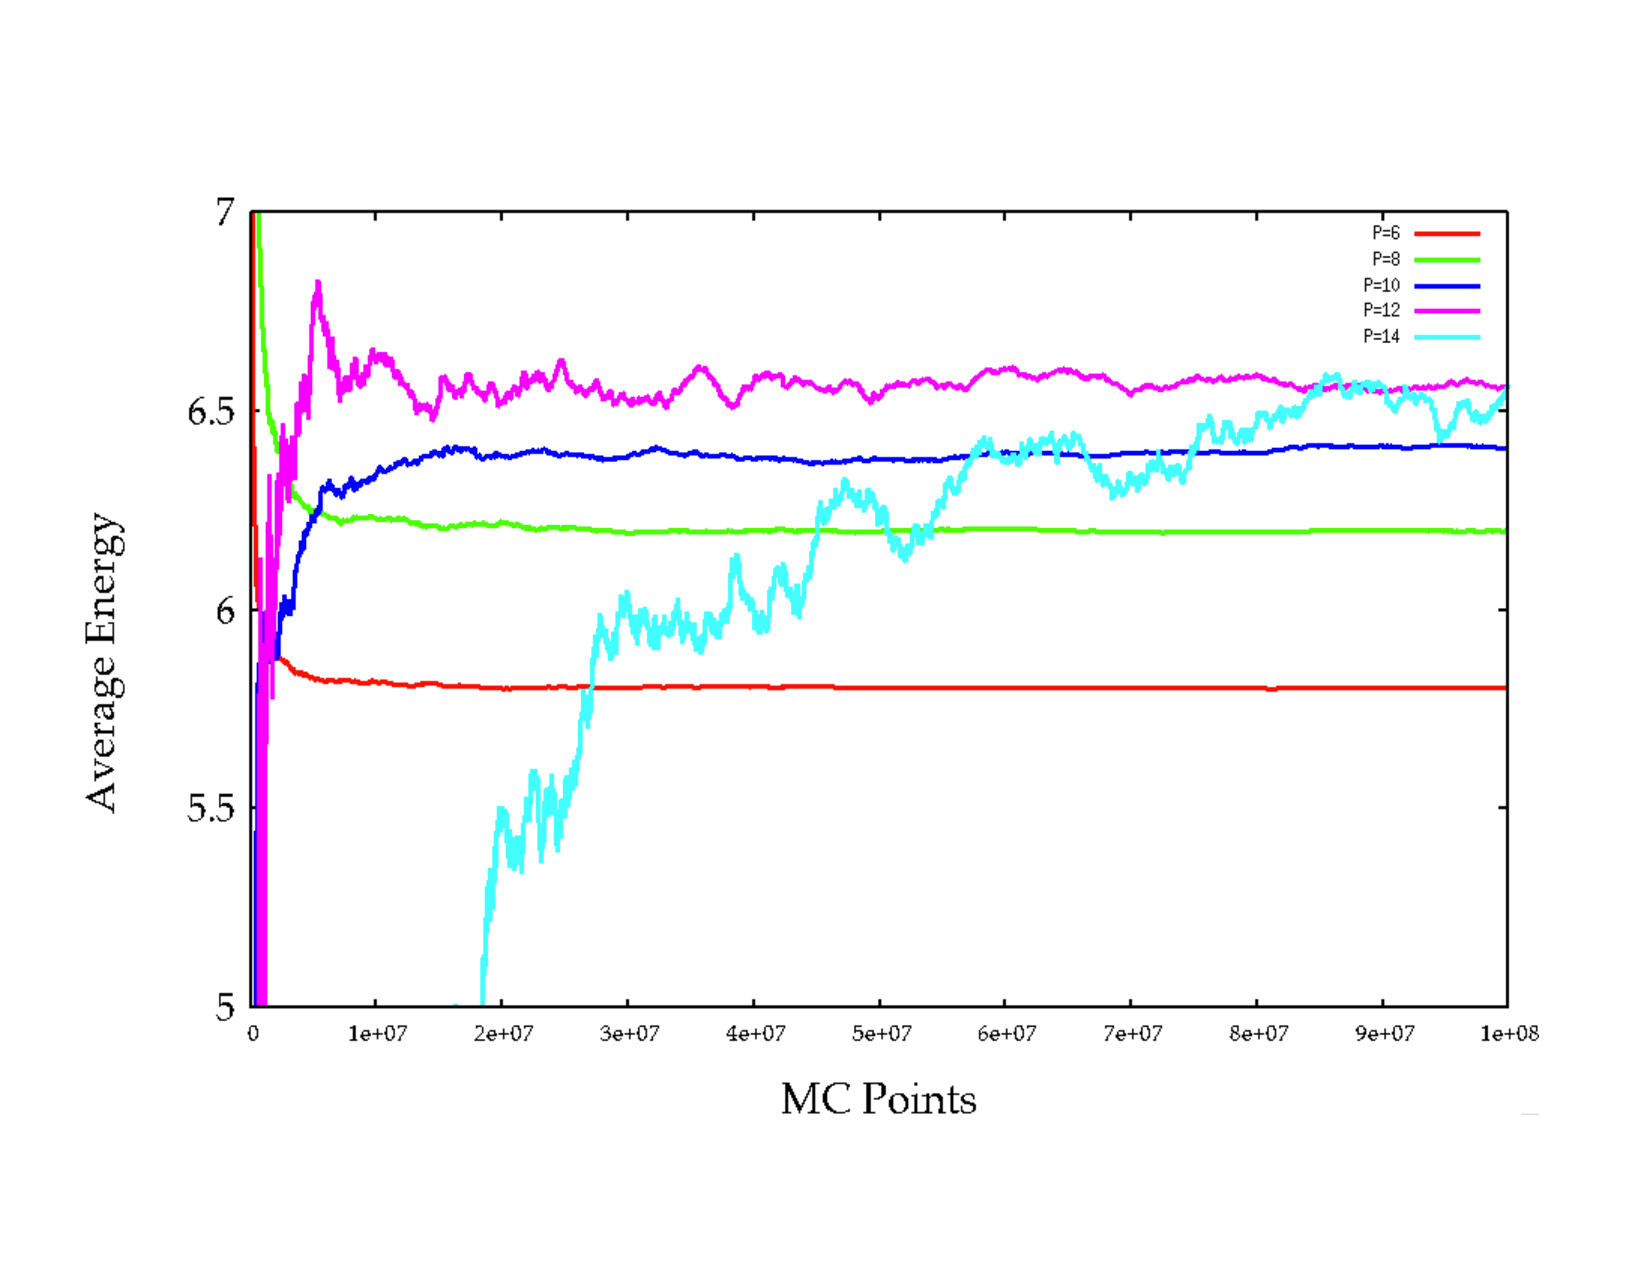
\includegraphics[scale=0.4]{avginstantonE}
\vspace{-0.1in}
\caption{Average energy bead convergence as a function of MC points }
\label{fig:avginstantonE}
\end{figure}

We find the instanton path corresponding to this system to be in reasonable agreement with the exact quantum instanton calculation reported by Cao and Voth ~\cite{CAO1995}. Disappointingly, our method of averaging instantaneous instanton configurations introduces arbitrary discrepancies in the which bead assumes the minimum value in individual instanton configurations. This causes the average minimum value to be located slightly above the minimum value reported by Cao and Voth ~\cite{CAO1995}



\begin{figure}[h!]
\vspace{-0.1in}
\centering
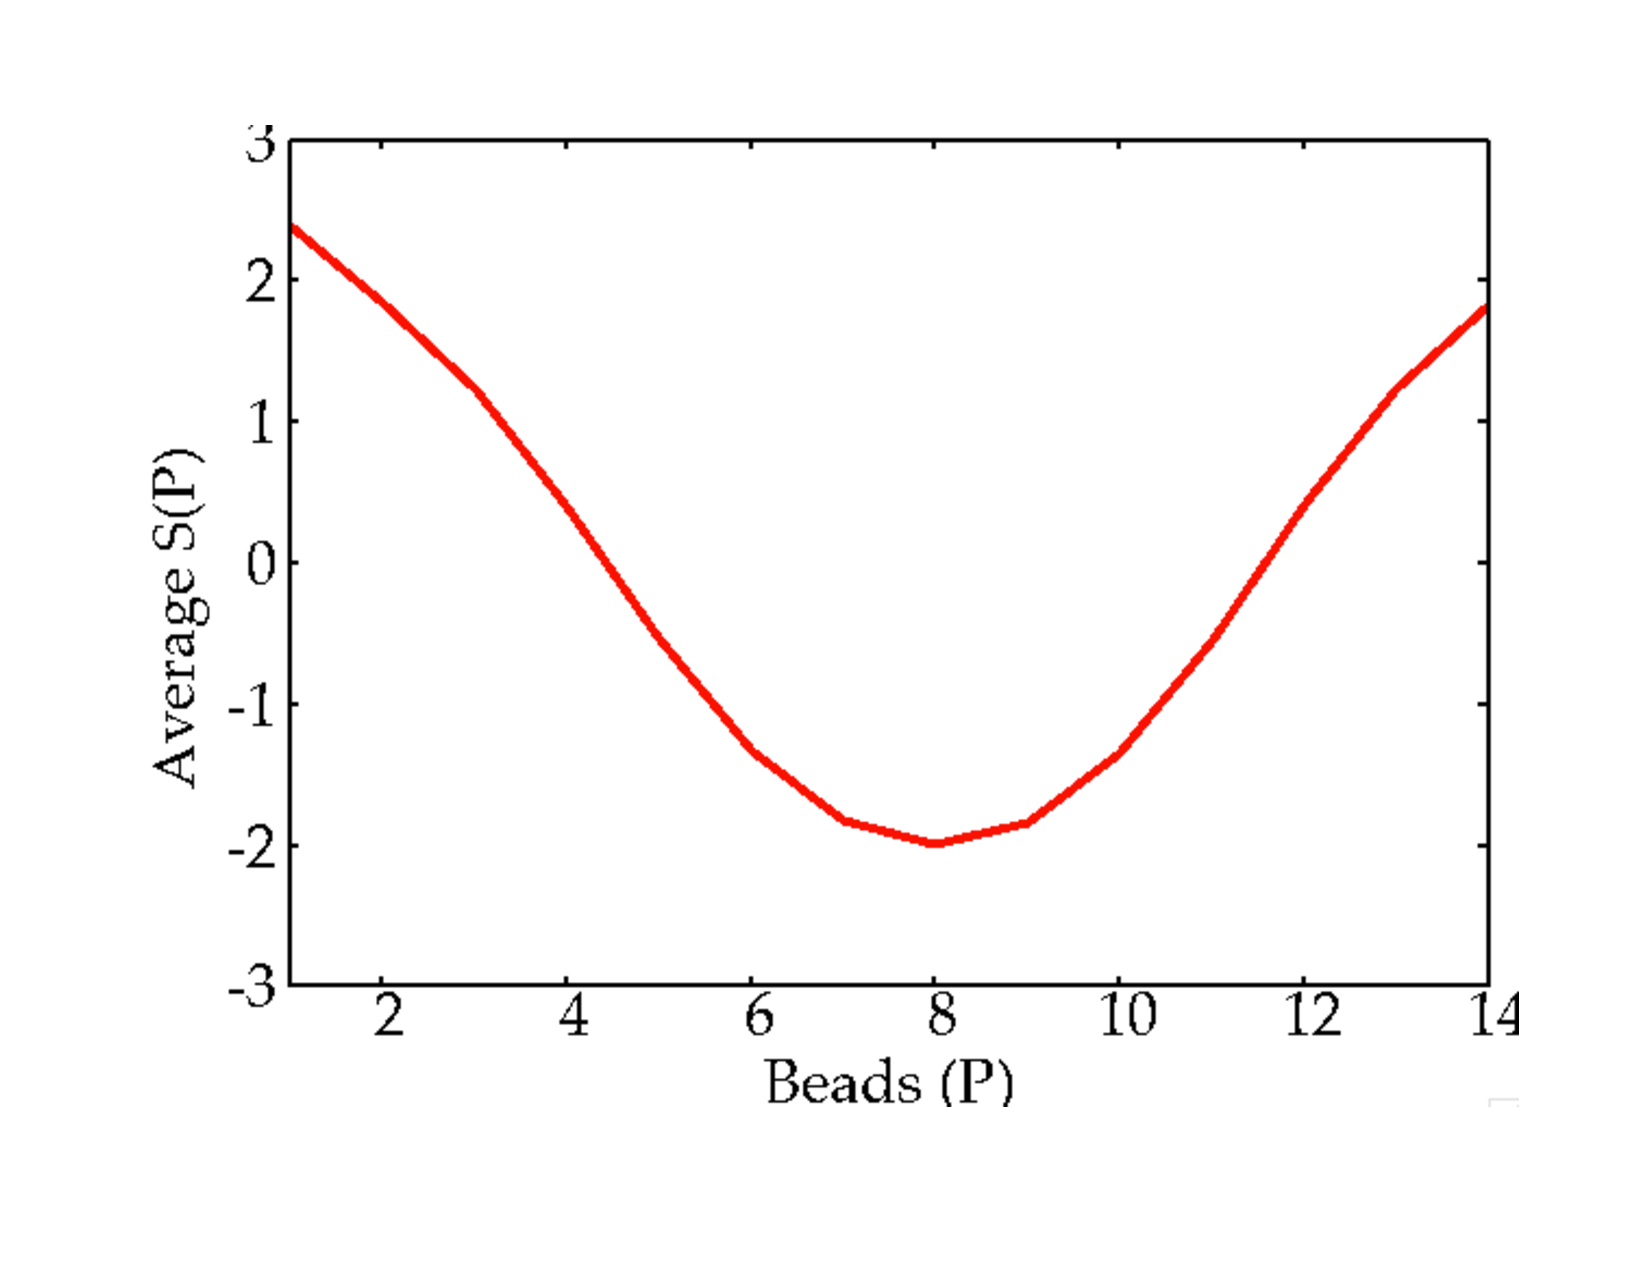
\includegraphics[scale=0.4]{instanton14b}
\vspace{-0.1in}
\caption{The nonadiabatic instanton trajectory plotted as a function of imaginary time }
\label{fig:instanton14b}
\end{figure}
We also calculate the average semiclassical population for this system and plot each bead population throughout the course of the MC simulation. As the simulation approaches convergence with respect to the number of MC points the population of state 1 (shown in red in Fig. 5.4) and the population of state 2 (shown in green in Fig 5.4) approach equality. This suggests that constraining the ring polymer centroid to the barrier constrains the average electronic population of each bead to be equal. 
\begin{figure}[h!]
\vspace{-0.2in}
\centering
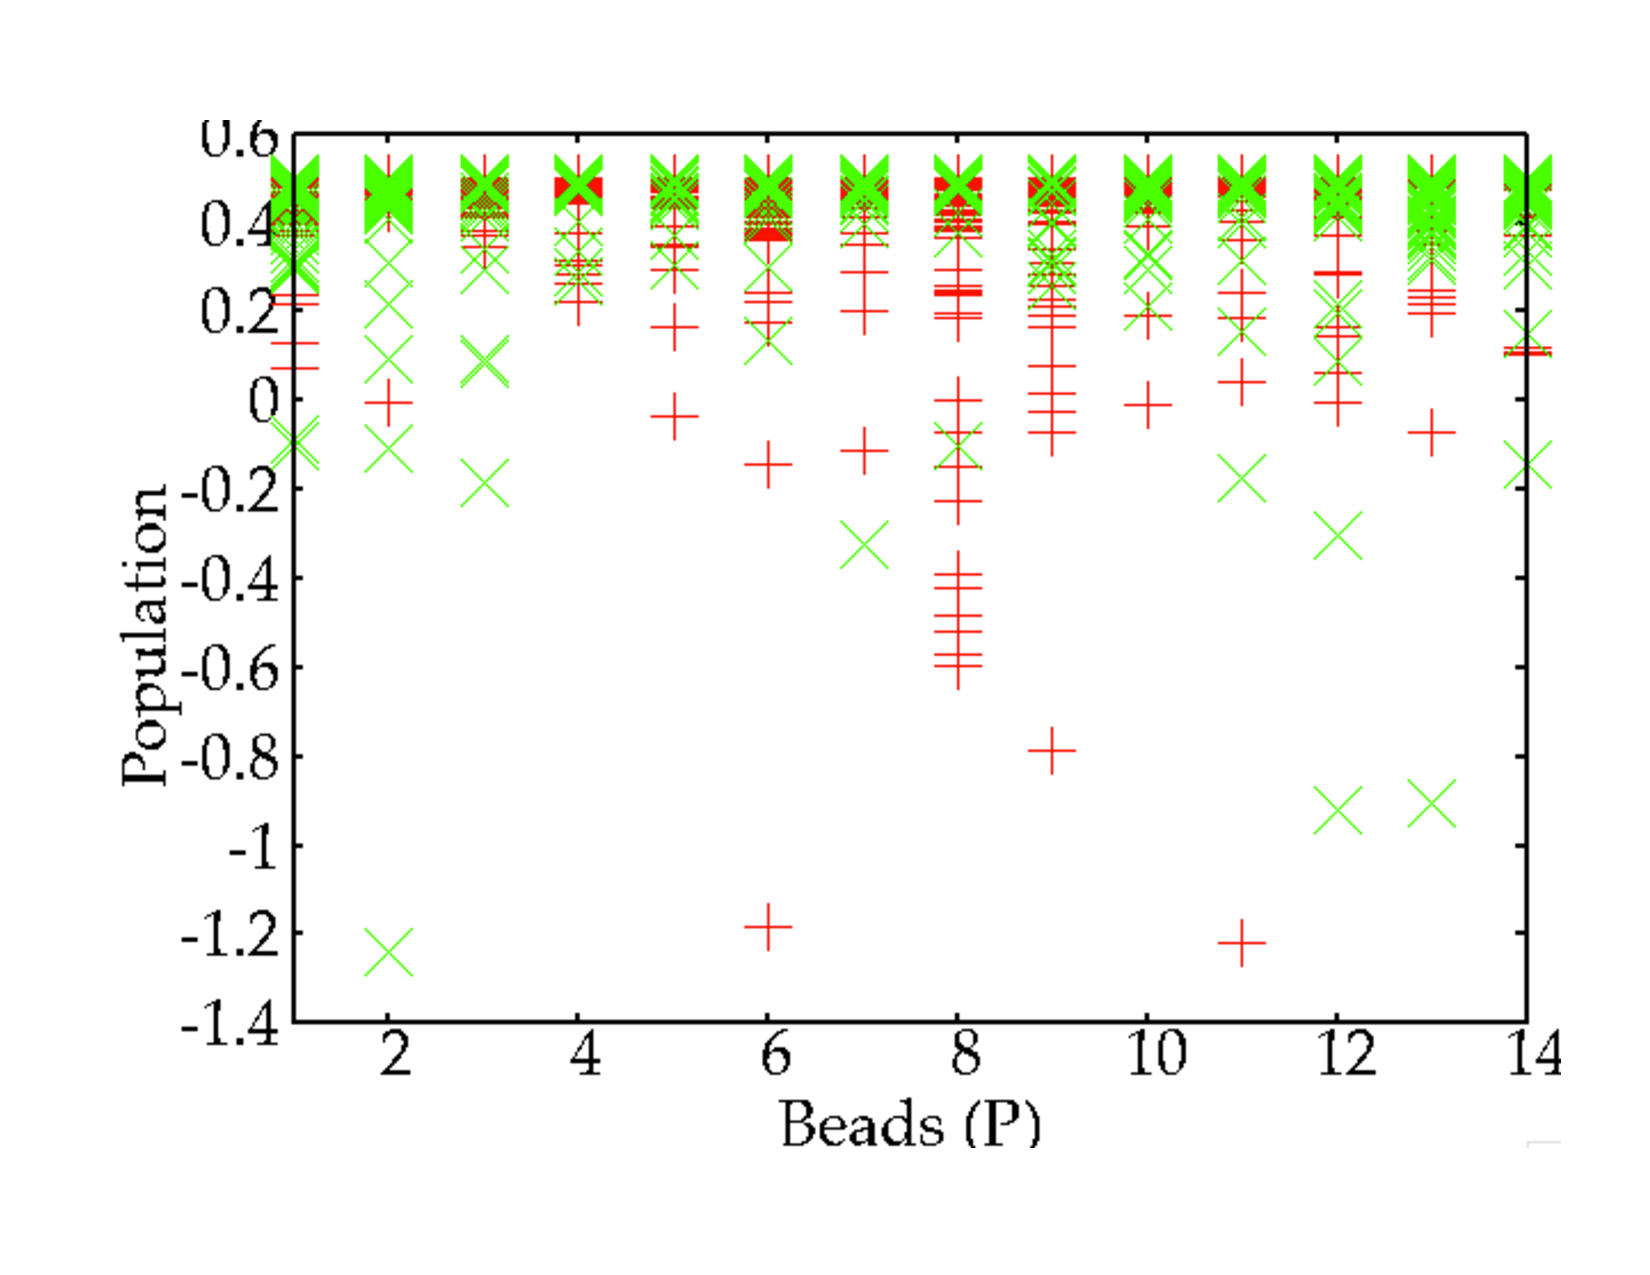
\includegraphics[scale=0.4]{avgpop}
\vspace{-0.2in}
\caption{Average Semiclassical Population with the population of state 1 (shown in red) and state 2 (shown in green) over the course of the MC simulation}
\label{fig:avgpop}
\end{figure}


In order to demonstrate why the minimum value of the averaged instanton configuration is slightly greater than the reported value, we plot instantaneous instanton configurations in Fig (5.5). As mentioned before, the arbitrary choice of making the "bead 1" have the maximum value causes discrepancies in which bead number assumes the minimum value in each instantaneous instanton configuration. The bead number with minimum value shifts between bead 6-10 causing bead 8 (which should have the minimum value) to be on average at a position slightly greater than the minimum value reported by Cao and Voth. 
\begin{figure}[h!]
\vspace{-0.2in}
\centering
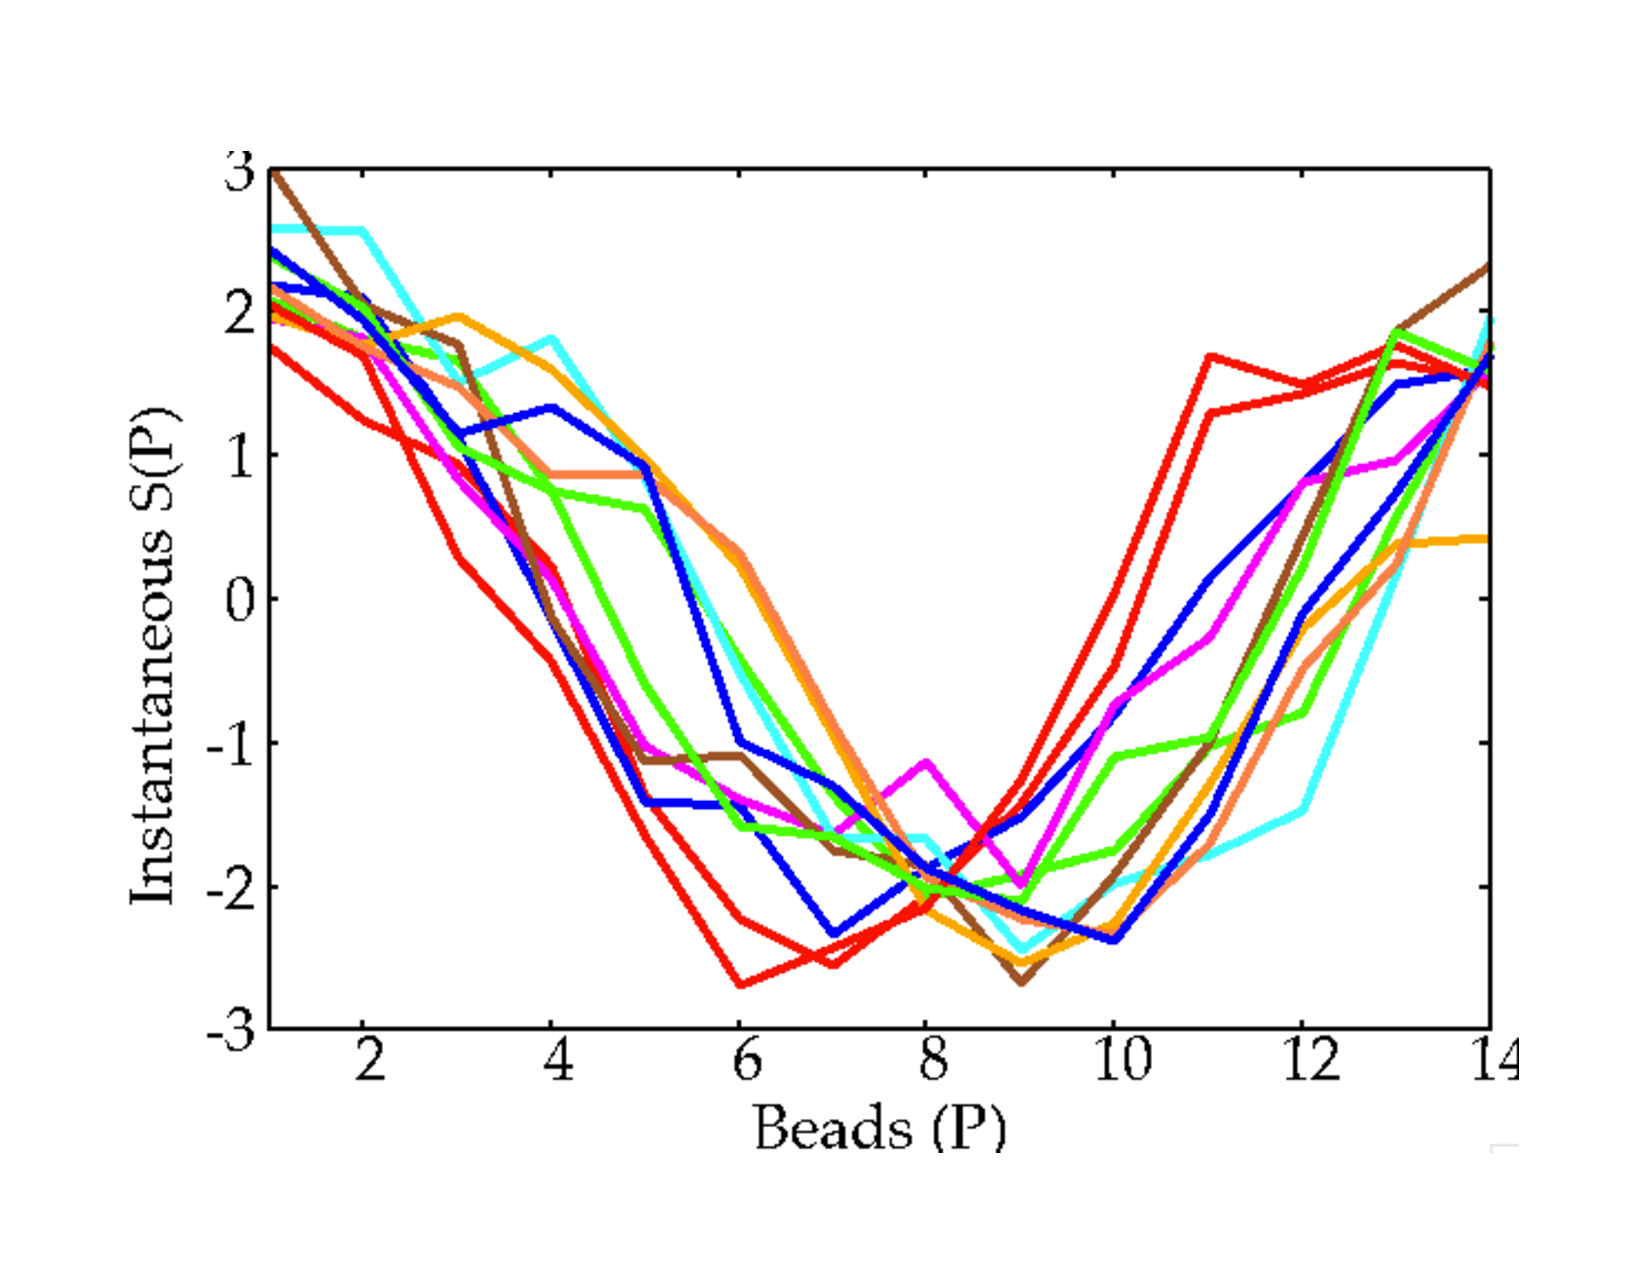
\includegraphics[scale=0.4]{instantaneousS}
\vspace{-0.2in}
\caption{Instantaneous instanton trajectories}
\label{fig:instantaneousS}
\end{figure}

\subsection{Summary}

We calculated the average instanton configuration using the QBD corresponding to the MV-RPMD Hamiltonian discussed throughout this study. While the average instanton is in reasonable agreement with the exact calculation reported by Cao and Voth ~\cite{CAO1995}, we find the average minimum value of the instanton path to be slightly greater than the reported figure. We attribute this to an artifact of the our averaging algorithm. Our choice to make the first bead the most positive, while reordering the remaining beads contiguously causes an artificial shift in the beads assigned to the minimum value of instantaneous paths. We see this from analyzing instantaneous instanton trajectories. While the instantaneous instanton paths have the correct minimum value, there is an ambiguity in which beads gets assigned the minimum values such that at any point in the Monte Carlo simulation bead 6-10 can have the minimum value while we'd expect the minimum to be located at bead 8 for a 14-bead calculation. Possible solutions to this issue may include initializing the PIMC simulation such that the RP solvent beads have the correct instanton configuration. Another possible solution is simulated annealing, where we run a PIMC simulation at a significantly higher temperature and initialize subsequent calculations with the converged high temperature RP configuration.

\section{MF-RPMD Rate Theory}
In the past MF-RPMD has been used to approximate the rate of ET in the condensed phase. It is known that because MF-RPMD approximates nuclear dynamics along a mean potential energy surface, it neglects fluctuation in electronic degrees of freedom. This approximation works well in multi-state system with strong coupling between states. In the MF-RPMD approximation, electronic motion is assumed to be significantly faster than nuclear motion which amounts to nuclear motion moving on an averaged potential surface. In strongly coupled systems this is precisely the case, where electronic transition between states are so rapid nuclear motion is approximately moving on an averaged surface. The MF-RPMD approximation fails when electronic and nuclear motion are on comparable timescales which corresponds to the nonadiabatic regime (weak coupling). This is due to the fact that MF-RPMD does not correctly account for fluctuations in electronic degrees of freedom and subsequently poorly approximates nuclear motion. As a result, MF-RPMD has be widely ignored as a viable method for the simulation nonadiabatic charge and energy transfer processes. 

A former member of our group developed two remedies to the inaccuracies in MF-RPMD ~\cite{JD2016}. The first accounts for the fact that in MF-RPMD, the probability of forming "kink" configurations (probabilities of forming electronic transition states) are not correctly accounted for the the MF-RPMD flux-side TCF expression. By correctly accounting for electronic transition state probabilities in MF-RPMD rate calculation, ET rates across a full range of coupling strengths were accurately approximated. While modifying MF-RPMD such that it can reproduce nonadiabatic ET rates is an impressive feat, the probabilities of forming kinks are introduced in a mathematically inconsistent manner. Further, this method failed to capture ET in the inverted regime. 

The second remedy was to introduce a population reaction coordinate, defined as the difference in product and reactant populations. This method resulted in the accurate rate calculation of ET across a full range of coupling strengths and in regimes outside of the normal regime. Despite this feat, MF-RPMD defined in terms of the population coordinate still failed to give quantitative agreement with FGR rate calculations in the inverted regime. A further issue is MF-RPMD's limitation to single particle processes. 

The following section outlines MV-RPMD rate theory developments which may alleviate some of the inherent issues with MF-RPMD and hopefully will lead to its application of general multi-level/multi-particle nonadiabatic systems in the condensed phase. 

 \subsection{MV-RPMD Flux-side TCF: Solvent Reaction coordinate}
The Bennett-Chandler expression for the rate constant is,
\begin{equation}
k= \frac{\langle \dot{\xi}_0  h(\dot{\xi}_0) \rangle_c \langle \delta (\xi_0 -\xi^{\dagger})\rangle}{\langle h(\xi^{\dagger} -\xi_0)\rangle} \times \lim_{t \to \infty} \frac{\langle \dot{\xi}_0 h(\xi_t -\xi^{\dagger}) \rangle_c}{\langle \dot{\xi}_0  h(\dot{\xi}_0) \rangle_c \langle \delta (\xi_0 -\xi^{\dagger})\rangle}.
\end{equation}

canceling the numerator and denominator in the expression we get, 

\begin{equation}
k= \lim_{t \to \infty}\frac{\langle \dot{\xi}_0 h(\xi_t -\xi^{\dagger}) \rangle_c}{\langle h(\xi^{\dagger} -\xi_0)\rangle} 
\end{equation}

The rate is defined in terms of a one-dimensional reaction coordinate $\xi$. Following the traditional mean field RPMD approach we define $\xi$ as a function of the solvent polarization bead average, also called the ring polymer center of mass (COM), $\xi = \bar{R} = 1/N\sum_{\alpha=1}^{N} R_{\alpha}$, where the transition state, the reactant well, and the product well correspond to $\bar{R}=R^{\dagger}$, $\bar{R}\leq R^{\dagger}$, and $\bar{R}\geq R^{\dagger}$ respectively. The transition state  $R^{\dagger}$ corresponds to the point of degeneracy between the two states. The rate can then be expressed as,

\begin{equation}
k= \lim_{t \to \infty}\frac{\langle \dot{\bar{R}}_0 h(\bar{R}_t -R^{\dagger}) \rangle_c}{\langle h(R^{\dagger} -\bar{R}_0)\rangle} 
\end{equation}


The rate constants calculated using the solvent polarization as the reaction coordinate, in the MF-RPMD framework, has been shown to severely overestimate the rate in the weak coupling regime ~\cite{JD2016}. This is because the rate expression neglects the probability of forming electronic transition states which is proportional to the coupling squared. This also fails to accurately capture reaction rates in the inverted regime.  



\begin{figure}[h!]
\vspace{-0.1in}
\centering
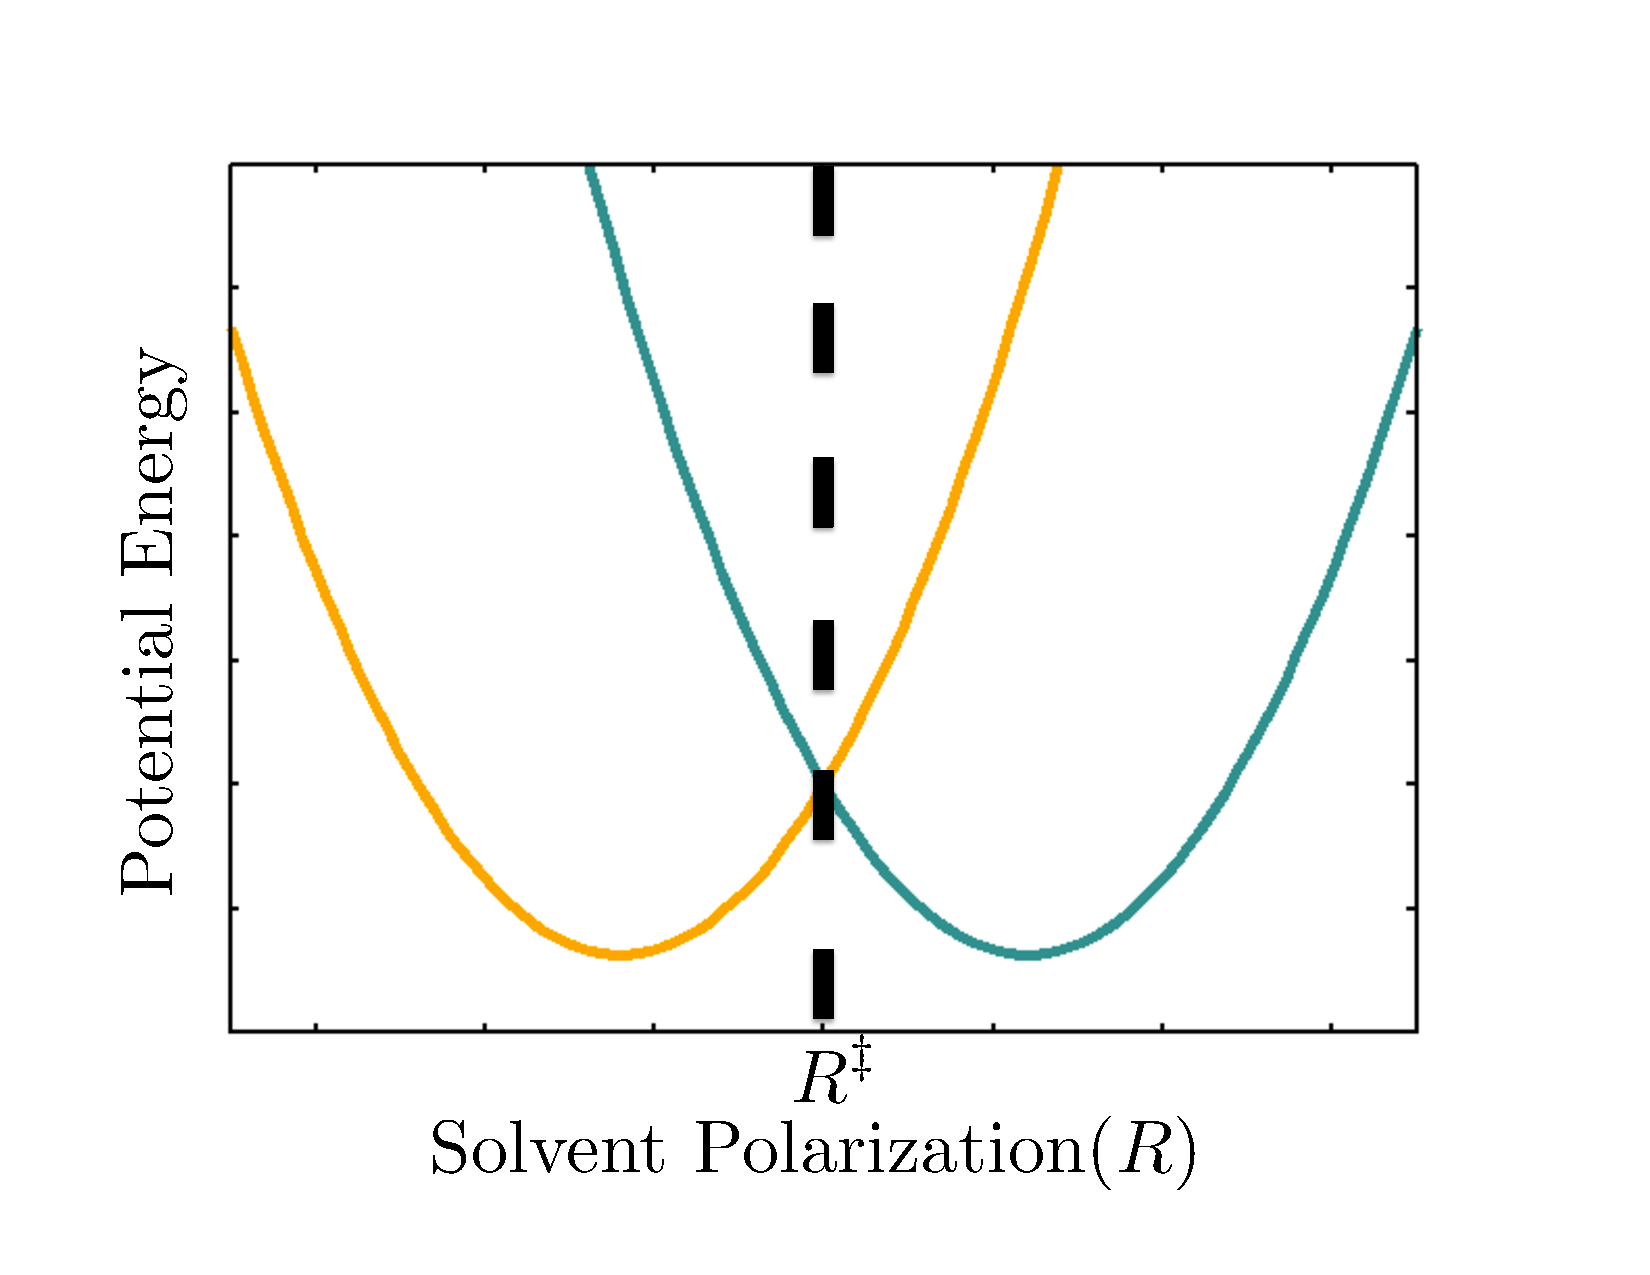
\includegraphics[scale=0.4]{schematicpot}
\vspace{-0.1in}
\caption{A schematic of the two-state electron transfer system in the adiabatic basis. The yellow curve is the reactant well and the green curve is the product and both are functions of solvent polarization. The black dashed line corresponds the the reaction transition state $(R^{\ddagger})$}.
\label{fig:schematicpot}
\end{figure}
In the MV-RPMD representation, unlike MF-RPMD, the statistical sampling and dynamics include explicit electronic state information, as well as the interaction between electronic states and nuclei in the $\Gamma$ matrix defined in Eq. (2.42). Within the MV-RPMD framework the rate cate be calculated piecewise as, 

\begin{equation}
 k=\lim_{t \to \infty}\frac{\langle \dot{\bar{R}}_0 h(\bar{R}_t -R^{\dagger}) \rangle_c}{\langle \textrm{sgn}(\Theta)\rangle_c} \times \frac{\langle \textrm{sgn}(\Theta)\rangle}{\langle h(R^{\dagger} -\bar{R}_0)\rangle} 
\end{equation}

where the left quantity is a dynamic calculation where initial RP configurations are sampled such that $\bar{R} = 1/N\sum_{\alpha=1}^{N} R_{\alpha}=0$ . Trajectories launched from this ensemble of initial configurations can be used to calculated flux-side TCF  defined by the solvent polarization coordinate. The time dependent product heaviside function (left quantity in Eq. 6.15),  $h(\bar{R}_t -R^{\dagger})$,  is, 

\begin{equation}
  h(\bar{R}_t -R^{\dagger})=\left\{
     \begin{array}{ll}
     1 & \textrm{if} \quad \bar{R}_t>0 \quad \textrm{products}\\
     0 &  \textrm{if} \quad  \bar{R}_t<0 \quad \textrm{reactants}
    \end{array}\right.
    \label{eq:hs}
\end{equation}
The static, reactant heaviside function (right quantity in Eq. 6.15) defined in terms of solvent polarization is, 
\begin{equation}
h(R^{\dagger} -\bar{R}_0)=\left\{
     \begin{array}{ll}
     1 & \textrm{if} \quad \bar{R}_0<0 \quad \textrm{products}\\
     0 &  \textrm{if} \quad  \bar{R}_0>0 \quad \textrm{reactants}
    \end{array}\right.
    \label{eq:hs}
\end{equation}


\section{MV-RPMD Flux-side TCF: Population Reaction coordinate}
Next we consider the reaction rate defined in terms of the population coordinate. The reaction coordinate  is defined as $\xi = \Delta \mathcal{P}$. Using this reaction coordinate the transition state, the reactant well, and the product well correspond to $\Delta \mathcal{P}=0$, $\Delta \mathcal{P}=-1$, and $\Delta \mathcal{P}=1$ respectively. The rate can then be expressed as,

\begin{equation}
k= \lim_{t \to \infty}\frac{\langle \dot{\Delta \mathcal{P}}_0 h(\Delta \mathcal{P}_t) \rangle_c}{\langle h(\Delta \mathcal{P}_0)\rangle} 
\end{equation}
Where we define $\xi = \Delta \mathcal{P}$ as the difference in bead population of the two electronic states, 
\begin{equation}
    \Delta \mathcal{P}=\left\{
     \begin{array}{ll}
     1 & \textrm{reactant}\\
     0 & \textrm{transition state}\\
     -1& \textrm{product}
    \end{array}\right.
    \label{eq:hs}
\end{equation}

We run two separate simulations where we calculate, 

\begin{equation}
 \lim_{t \to \infty}\frac{\langle \dot{\Delta \mathcal{P}}_0 h(\Delta \mathcal{P}_t) \rangle_c}{\langle \textrm{sgn}(\Theta)  \rangle_c} \times\frac{\langle \textrm{sgn}(\Theta)\rangle}{\langle  h(\Delta \mathcal{P}_0)\rangle}
\end{equation}

where the left quantity is a dynamic calculation where initial configurations are sampled with a constraint on the semiclassical population estimator, $\mathcal{P}_1^{\textrm{SC}} =\mathcal{P}_2^{\textrm{SC}}=0.5$, for each bead in the RP. Trajectories launched from the ensemble of initial constrained configurations can be used to calculate the flux-side TCF defined by the population reaction coordinate.  The population reaction coordinate is defined in terms of the Boltzmann population as, 

\begin{equation}
\Delta \mathcal{P}=\frac{\Gamma_2-\Gamma_1}{\textrm{tr}[\Gamma]}
\end{equation}

The population reaction coordinate is defined in terms of the semiclassical estimator as, 
\begin{equation}
\Delta \mathcal{P}= \mathcal{P}_2^{\textrm{SC}}-\mathcal{P}_1^{\textrm{SC}}
\end{equation} 
 The derivative of the population difference is,
 
\begin{equation}
\dot{\Delta \mathcal{P}}_0= ([x_{\alpha}]_2+[p_{\alpha}]_2-[x_{\alpha}]_1-[p_{\alpha}]_1)
\end{equation}
and the time dependent product and static reactant heaviside functions, respectively are,
\begin{equation}
   h( \Delta \mathcal{P}_t)=\left\{
     \begin{array}{ll}
     1 & \textrm{if} \quad \mathcal{P}_2(t)>\mathcal{P}_1(t)\\
     0 &  \textrm{if} \quad  \mathcal{P}_2(t)<\mathcal{P}_1(t)
    \end{array}\right.
    \label{eq:hs}
\end{equation}
and, 

\begin{equation}
   h( \Delta \mathcal{P}_0)=\left\{
     \begin{array}{ll}
     1 & \textrm{if} \quad \mathcal{P}_1(0)>\mathcal{P}_2(0)\\
     0 &  \textrm{if} \quad  \mathcal{P}_1(0)<\mathcal{P}_2(0)
    \end{array}\right.
    \label{eq:hs}
\end{equation}
which both can be used with the Boltzmann or semiclassical estimator. 

\section{MV-RPMD Flux-side TCF: Wigner Transform of Flux Operator}
A final expression to consider is the flux-side TCF defined in terms of the Wigner transform of the flux operator. 
We start by considering a two-state Hamiltonian operator defined by, 

\begin{equation}
\hat{H}=V_{11} |1\rangle \langle 1| +V_{22} |2\rangle \langle 2|+V_{12} |1\rangle \langle 2|+V_{21} |2\rangle \langle 1|
\end{equation}

\begin{equation}
\hat{F} = \frac{i}{\hbar} [\hat{H}, \mathcal{P}]
\end{equation}

where,

\begin{equation}
 \mathcal{P}=  |2\rangle \langle 2|
\end{equation}


\begin{eqnarray}
&&\hat{F} = \frac{i}{\hbar} (V_{11} |1\rangle \langle 1|2\rangle \langle 2|+V_{22}|2\rangle \langle 2|2\rangle \langle 2|
\\
\nonumber
&&+
V_{12}|1\rangle \langle 2|2\rangle \langle 2|+V_{21}|2\rangle \langle 1|2\rangle \langle 2|
\\
\nonumber
&&- 
(|2\rangle \langle 2|1\rangle \langle 1|V_{11}+|2\rangle \langle 2|2\rangle \langle 2|V_{22}
\\
\nonumber
&&+
|2\rangle \langle 2|1\rangle \langle 2|V_{12}+|2\rangle \langle 2|2\rangle \langle 1|V_{21})
\end{eqnarray}


since $ \langle 2|1\rangle= \langle1 |2\rangle=0$ and $ \langle 2|2\rangle= \langle1 |1\rangle=1$ we have, 

\begin{equation}
\hat{F} = \frac{i}{\hbar}(V_{12} |1\rangle \langle 2|-V_{21}|2\rangle \langle 1|)
\end{equation}

if we map discrete states to creation and annihilation operators such that $a^{\dagger}_n a_m=  |n\rangle \langle m|$ we have,

\begin{equation}
\hat{F} =a^{\dagger}_1 a_2 V_{12} - a^{\dagger}_2 a_1 V_{21}
\end{equation}

and if we note that $a^{\dagger}_n= \frac{1}{\sqrt{2}}(\hat{x}_n- i\hat{p}_n)$ and $a_m= \frac{1}{\sqrt{2}}(\hat{x}_m+ i\hat{p}_m)$ and if we consider systems where $V_{12}=V_{21}$ we get 8 terms in the flux expression,

\begin{equation}
\hat{F} = \frac{i}{\hbar}[(\hat{x}_1- i\hat{p}_1)(\hat{x}_2+ i\hat{p}_2)V_{12} - (\hat{x}_2- i\hat{p}_2)(\hat{x}_1+ i\hat{p}_1)V_{12}] 
\end{equation}

and expanding we get, 
\begin{eqnarray}
&&\hat{F} = \frac{i}{\hbar}[V_{12}(\hat{x}_1\hat{x}_2-i\hat{p}_1\hat{x}_2+i\hat{x}_1\hat{p}_2-i^2\hat{p}_1\hat{p}_2)
\\
\nonumber
&&-
V_{12}(\hat{x}_2\hat{x}_1-i\hat{p}_2\hat{x}_1+i\hat{x}_1\hat{p}_2-i^2\hat{p}_2\hat{p}_1)]
\end{eqnarray}
where the knowledge of the Wigner transform of two of the expressions gives sufficient information for the Wigner transform of the other six. Following the prescription outlined in the derivation of the semiclassical estimator~\cite{hel16} (See Appendix) we have,

\begin{equation}
[\hat{x}_1\hat{x}_2]_W=\int d \Delta x_1 \int d \Delta x_2 \langle {x}_1-\Delta {x}_{1}/{2},{x}_2-\Delta {x}_{2}/{2} | \hat{x}_1\hat{x}_2| {x}_1+\Delta {x}_{1}/{2},{x}_2+\Delta {x}_{2}/{2} \rangle e^{i(p_1\Delta x_1+p_2\Delta x_2)}
\end{equation}



\begin{equation}
[\hat{x}_1\hat{x}_2]_W=\int d \Delta x_1 \int d \Delta x_2 (x_1 +\Delta x_1/2) (x_2 +\Delta x_2/2)\delta (\Delta x_1) \delta (\Delta x_2) e^{i(p_1\Delta x_1+p_2\Delta x_2)}= x_1 x_2
\end{equation}

Also noting that $[p_n,x_m]=0$ for the second term, $-i\hat{p}_1\hat{x}_2$, we have,

\begin{eqnarray}
&&[-i\hat{p}_1\hat{x}_2]_W=  -i\int dp_1 \int dp_2  \int d \Delta x_1 \int d \Delta x_2  \\ 
\nonumber
&& \times
\langle {x}_1-\Delta {x}_{1}/{2},{x}_2-\Delta {x}_{2}/{2} |  \\ 
\nonumber
&& \times
\hat{p}_1\hat{x}_2| {x}_1+\Delta {x}_{1}/{2},{x}_2+\Delta {x}_{2}/{2} \rangle
\\ 
\nonumber
&& \times
 e^{i(p_1\Delta x_1+p_2\Delta x_2)}
\end{eqnarray}
since 

\begin{equation}
\hat{x}_2| {x}_1+\Delta {x}_{1}/{2},{x}_2+\Delta {x}_{2}/{2} \rangle=({x}_2-\Delta {x}_{2}/{2})| {x}_1+\Delta {x}_{1}/{2},{x}_2+\Delta {x}_{2}/{2} \rangle
\end{equation}

and inserting a complete set of momentum states $\mathcal{I}=\int dp'_1 \int dp'_2 |p'_1, p'_2\rangle \langle p'_1, p'_2 |$. 
\begin{eqnarray}
&&[-i\hat{p}_1\hat{x}_2]_W=  -i\int dp'_1 \int dp'_2  \int d \Delta x_1 \int d \Delta x_2  ({x}_2-\Delta {x}_{2}/{2})\\ 
\nonumber
&& \times
\quad\langle {x}_1-\Delta {x}_{1}/{2},{x}_2-\Delta {x}_{2}/{2} |\hat{p}_1 |p'_1, p'_2\rangle \\ 
\nonumber
&& \times
 \langle p'_1, p'_2 | {x}_1+\Delta {x}_{1}/{2},{x}_2+\Delta {x}_{2}/{2} \rangle \\ 
\nonumber
&& \times
  e^{i(p_1\Delta x_1+p_2\Delta x_2)}
\end{eqnarray}

and since, 




\begin{equation}
\hat{p}_1 |p'_1, p'_2\rangle={p}_1 |p'_1, p'_2\rangle
\end{equation}
we have 
\begin{eqnarray}
&&[-i\hat{p}_1\hat{x}_2]_W=  -i\int dp'_1 \int dp'_2  \int d \Delta x_1 \int d \Delta x_2  ({x}_2-\Delta {x}_{2}/{2})p_1\\ 
\nonumber
&& \times
\quad\langle {x}_1-\Delta {x}_{1}/{2},{x}_2-\Delta {x}_{2}/{2} |p'_1, p'_2\rangle \\ 
\nonumber
&& \times
 \langle p'_1, p'_2 | {x}_1+\Delta {x}_{1}/{2},{x}_2+\Delta {x}_{2}/{2} \rangle  \\ 
\nonumber
&& \times
 e^{i(p_1\Delta x_1+p_2\Delta x_2)}
\end{eqnarray}
and noting 
\begin{equation}
\langle {x}_1-\Delta {x}_{1}/{2},{x}_2-\Delta {x}_{2}/{2} |p'_1, p'_2\rangle =e^{ip'_1({x}_1+\Delta {x}_{1}/{2})}e^{ip'_2({x}_2+\Delta {x}_{2}/{2})}
\end{equation}
 we get, 

\begin{eqnarray}
&&[-i\hat{p}_1\hat{x}_2]_W= -i\int dp'_1 \int dp'_2  \int d \Delta x_1 \int d \Delta x_2 
 ({x}_2-\Delta {x}_{2}/{2})p_1
\\ 
\nonumber
&& \times
e^{ip'_1({x}_1+\Delta {x}_{1}/{2})}e^{ip'_2({x}_2+\Delta {x}_{2}/{2})}
\\ 
\nonumber
&& \times
e^{-ip'_1({x}_1-\Delta {x}_{1}/{2})}e^{-ip'_2({x}_2-\Delta {x}_{2}/{2})}
\\ 
\nonumber
&& \times
e^{i(p_1\Delta x_1+p_2\Delta x_2)}\\
\end{eqnarray}
and using the definition in Eq. (A.11) we find, 
\begin{eqnarray}
&&[-i\hat{p}_1\hat{x}_2]_W= -i\int dp'_1 \int dp'_2 \int d \Delta x_1 \int d \Delta x_2  ({x}_2-\Delta {x}_{2}/{2})p_1
\\ 
\nonumber
&& \times
e^{ip'_1\Delta {x}_{1}}e^{ip'_2\Delta {x}_{2}}
\\ 
\nonumber
&& \times
e^{i(p_1\Delta x_1+p_2\Delta x_2)}
\\ 
\nonumber
&&=
\int d \Delta x_1 \int d \Delta x_2  ({x}_2-\Delta {x}_{2}/{2})p_1
\\ 
\nonumber
&& \times
\delta(\Delta {x}_{1})\delta(\Delta {x}_{2})
\\ 
\nonumber
&& \times
e^{i(p_1\Delta x_1+p_2\Delta x_2)}= -i  p_1x_2
\end{eqnarray}

so we have, 

\begin{equation}
[-i\hat{p}_1\hat{x}_2]_W=-i  p_1x_2
\end{equation}

Following similar algebra for the remaining terms, and noting that $x_n$ and $p_n$ are now scalars we get, 
\begin{eqnarray}
&&[\hat{F}]_W  = \frac{i}{\hbar}[V_{12}({x}_1{x}_2-i{p}_1 {x}_2+i {x}_1{p}_2+ {p}_1 {p}_2)
\\ 
\nonumber
&&-V_{12}({x}_2 {x}_1-i{p}_2{x}_1+i{x}_1 {p}_2+{p}_2 {p}_1)]
\\ 
\nonumber
&&=
 \frac{2i}{2\hbar}[V_{12}(-i{p}_1 {x}_2+i {x}_1{p}_2]
 \\ 
\nonumber
&&=
 \frac{1}{\hbar}[V_{12}({p}_1 {x}_2- {x}_1{p}_2)]
\end{eqnarray}

so finally we have a continuous expression for the flux in terms of conjugate variables, 
\begin{equation}
[\hat{F}]_W  =  \frac{1}{\hbar}[V_{12}({p}_1 {x}_2- {x}_1{p}_2)]
\end{equation}


\subsection{Summary}
In this section we discussed limitations of MF-RPMD nonadiabatic rate calculations and why one might be interested in the formulation of an MV-RPMD rate theory. First we noted that rate calculations formulated in terms of solvent polarization COM, in the MF-RPMD formalism, do not work well at capturing nonadiabatic reaction rates. This is because constraining initial electronic population does sufficiently constrain nuclear coordinates and constraining nuclear coordinates do not sufficiently constrain population. This results in the requirement of a double constraint in population and nuclear coordinates, which proves to be numerically demanding in practice. The correction to the rate is therefore introduced by multiplying the estimator for flux-side by the probability of forming RP "kinks" which corresponds to the probability of forming electronic transition states. While this correction to the rate calculation allowed for the use of MF-RPMD to calculate rates across a full range of coupling strengths, it is mathematically inconsistent and fails to capture ET in the inverted regime.
In an effort to remedy this inconsistency, the population difference coordinate was developed. The population coordinate distinguishes between reactants and products in all regimes of ET and gives the desired turnover for ET in the inverted regime. Still given that this method restricts kink formation outside of the adiabatic crossing, it fails to quantitatively agree with the exact FGR rate calculation

We then sought to explore different formulations of the flux-side TCFs in the MV-RPMD formalism where "kink" probabilities are accounted for in a mathematically consistent manner. MF-RPMD is still limited to the description of single particle processes. 
Ideally we would like to be able to capture reaction rates across a full range of coupling strengths, and across all regimes while keeping our methods general for multi-electron systems. Further, if we wish to study the rate of photochemical reactions, MV-RPMD is ideal since it consistently treats discrete system states with continuous conjugate variables.

Working toward the goal of applying MV-RPMD to a rate calculation, we explore three MV-RPMD rate formulations. The first is the MV-RPMD flux-side TCF defined in terms of a solvent polarization reaction coordinate. The second is the MV-RPMD flux-side TCF defined in terms of a population difference reaction coordinate. Finally, we outline the derivation of the continuous representation of the flux operator (for a two-state system) which can be implemented in a flux-side MV-RPMD TCF calculation. In the future we hope to apply these MV-RPMD rate theories to rate calculations in nonadiabatic condensed phase systems. This will inform the development of an efficient yet general MV-RPMD rate theory that can be applied to multi-state systems across a wide range of coupling strengths and regimes. 


\chapter{Conclusions }
This dissertation focused on the extension and application of a nonadiabatic version of RPMD (MV-RPMD), which allowed for the accurate and efficient simulation of quantum mechanical reactions in the condensed phase. We started our discussion with a review of imaginary-time path integrals and the classical isomorphism that falls out of the path integral discretization of the QBD. This provides an exact, yet efficient, method for generating quantum statistics for systems in the condensed phase. 

Next we reviewed the real-time extension of the PI formalism, RPMD, which approximate Kubo-transformed thermal correlation functions and gives the exact result as $t\to0$. We then went on to discuss the details of the RPMD approximations, its limitations and motivations for its extension. While RPMD has been successfully applied to a wide range of chemical problem, it's inability to treat features like quantum coherence, multi-quantum particle processes, and multi-state processes necessitates efforts toward its extension. 


Our review of nonadiabatic extensions of RPMD motivated our discussion of MV-RPMD. In MV-RPMD we represent discrete system states with continuous variables by mapping to SEO states. We then take the Wigner Transform of the SEO states in order to represent our system with a quasi-probability distribution which allow us to sample continuous conjugate variables that can be integrated in classical EOMs. We also derive an improved QBD in the MV-RPMD framework by employed the symmetric trotter splitting of kinetic and potential energy operators. We demonstrate improved numerical stability in average energy bead convergence of a model ET system. 


To motivate our study of PCET using MV-RPMD, we review the model PCET systems that have been reported in the literature. The first was PCET modeled by capped Coulombic wells coupled to a proton double well in the presence of a solvent coordinate. RPMD bead convergence within this model depends on the proton and electron mass, which typically requires 32 beads and 1024 beads for converged dynamics respectively. The shortcoming of this model is its treatment of the electron and proton as unique particles. The next model studied was a proton double well coupled to discrete ET states coupled to a proton double well. Since we are working in the weak coupling (nonadiabatic) regime, the burden of bead convergence is dominated by the light proton mass, which requires 32 beads. In the MV-RPMD representation, the 32 bead requirement proves to be computationally demanding. We then turn to the method of quasi-diabatization in order to represent our PCET system with four discrete electron/proton states. This significantly reduces the number of beads required for convergence in equilibrium and dynamic simulations. We were able to demonstrate that MV-RPMD can be used to accurately distinguish between concerted and sequential PCET processes. 


In order to extend our application of MV-RPMD to nonadiabatic rate calculations in the condensed phase, we review two equivalent rate theories, the flux-side thermal correlation function and the Semiclassical "ImF" method. The latter has been shown to be equivalent to RPMD rate calculations in the deep tunneling regime which further shed light on the nature of the RPMD approximation. Knowing that the instanton is the imaginary-time periodic path around a reaction barrier, or the real-time path on an inverted potential barrier, we can use MV-RPMD to calculate the instanton configuration by sampling configurations at the barrier. We calculate the average instanton configuration for a spin-boson model in the weak coupling regime and found it to agree well with exact calculation reported in the literature. 

Finally, we reviewed RPMD rate theory and its past applications and motivated its extension. We then formulated two flux-side TCF expressions using the MV-RPMD formalism. The first involved a reaction coordinate defined by the solvent polarization COM where  dynamic trajectories are initialized such that the RP solvent polarization COM is constrained to the barrier. The second involves a population coordinate defined by the difference in the product and reactant population where the propagated product heaviside can either be defined in terms of the Boltzmann or the semiclassical population estimator. Finally we provide the derivation of the flux estimator which we can use within the MV-RPMD formalism to calculate a flux-side TCF. 


More recent work in our group has been toward finding the optimal dividing surface on the MV-RPMD effective potential (MV-RPMD instanton) for the calculation of nonadiabatic rates in the condensed phase ~\cite{SRINANTH18}. The development of a robust MV-RPMD rate theory that is applicable across a full range of coupling strengths and across all regimes will further the progress toward simulating and subsequently understanding complex charge and energy processes in the condensed phase. Deeper understanding of these process will inform the rational design of novel materials in renewable energy technologies. 
 

\appendix

\chapter{Chapter 1 of appendix}


\section{Derivation of Semiclassical Population estimator}
We start the derivation of the semiclassical population estimator with the following definitions,

\begin{equation}
\langle x|p\rangle = \frac{1}{(2\pi)^{1/2}}  e^{ipx} 
\end{equation}

\begin{equation}
\int \langle x|p\rangle \langle p|x'\rangle dp= \frac{1}{2\pi} \int e^{ip(x-x')} dp= \delta(x-x')
\end{equation}
and 
\begin{equation}
\int \delta (x)f(x)= f(0)
\end{equation}

if we have the operator $\hat{S}$, for the thermal population of a particular state $\alpha$, defined by
\begin{equation}
\hat{S}= \frac{1}{2}(\hat{x}_{\alpha}^2+\hat{p}_{\alpha}^2-1) 
\end{equation}

the wigner transform of $\hat{S}$ is,
\begin{equation}
[\hat{S}]_W=\int d {\Delta \bf{x}} \langle {\bf{x}}-\Delta \bf{x}/{2}| \hat{S} | {\bf{x}}+\Delta \bf{x}/{2} \rangle e^{i{\bf{p} \cdot \Delta x}}
\end{equation}

if we have $\alpha=1$, for a two-sate system
\begin{equation}
[\hat{x}_1^2]_W=\int d \Delta x_1 \int d \Delta x_2 \langle {x}_1-\Delta {x}_{1}/{2},{x}_2-\Delta {x}_{2}/{2} | \hat{x}_{1}^2 | {x}_1+\Delta {x}_{1}/{2},{x}_2+\Delta {x}_{2}/{2} \rangle e^{i(p_1\Delta x_1+p_2\Delta x_2)}
\end{equation}



\begin{equation}
[\hat{x}_1^2]_W=\int d \Delta x_1 \int d \Delta x_2 (x_1 +\Delta x_1/2)^2 \delta (\Delta x_1) \delta (\Delta x_2) e^{i(p_1\Delta x_1+p_2\Delta x_2)}= x_1^2
\end{equation}
since,

\begin{equation}
 \langle {x}_{\alpha}-\Delta {x}_{\alpha}/{2}|{x}_{\alpha}+\Delta {x}_{\alpha}/{2}\rangle= \delta (\Delta x_{\alpha})
\end{equation}


\begin{equation}
[\hat{p}_1^2]_W=\int d \Delta x_1 \int d \Delta x_2 \langle {x}_1-\Delta {x}_{1}/{2},{x}_2-\Delta {x}_{2}/{2} | \hat{p}_{1}^2 | {x}_1+\Delta {x}_{1}/{2},{x}_2+\Delta {x}_{2}/{2} \rangle e^{i(p_1\Delta x_1+p_2\Delta x_2)}
\end{equation}

and we insert a complete set of momentum states,

\begin{equation}
\mathcal{I}= \int dp'_1 \int dp'_2 |p'_1, p'_2\rangle \langle p'_1, p'_2 |
\end{equation}


\begin{eqnarray}
&&[\hat{p}_1^2]_W= \int dp'_1 \int dp'_2  \int d \Delta x_1 \int d \Delta x_2 \\ 
\nonumber
&& \times
\quad\langle {x}_1-\Delta {x}_{1}/{2},{x}_2-\Delta {x}_{2}/{2} | \hat{p}_{1}^2  |p'_1, p'_2\rangle \\ 
\nonumber
&& \times
 \langle p'_1, p'_2 | {x}_1+\Delta {x}_{1}/{2},{x}_2+\Delta {x}_{2}/{2} \rangle e^{i(p_1\Delta x_1+p_2\Delta x_2)}
\end{eqnarray}

\begin{eqnarray}
&&[\hat{p}_1^2]_W= \int dp'_1 \int dp'_2  \int d \Delta x_1 \int d \Delta x_2 
({p'}_{1}^2)
\\ 
\nonumber
&& \times
e^{ip'_1({x}_1+\Delta {x}_{1}/{2})}e^{ip'_2({x}_2+\Delta {x}_{2}/{2})}
\\ 
\nonumber
&& \times
e^{-ip'_1({x}_1-\Delta {x}_{1}/{2})}e^{-ip'_2({x}_2-\Delta {x}_{2}/{2})}
\\ 
\nonumber
&& \times
e^{i(p_1\Delta x_1+p_2\Delta x_2)}\\
\nonumber
&& = \int dp'_1 \int dp'_2 \int d \Delta x_1 \int d \Delta x_2 ({p'}_{1}^2)
\\ 
\nonumber
&& \times
e^{ip'_1\Delta {x}_{1}}e^{ip'_2\Delta {x}_{2}}
\\ 
\nonumber
&& \times
e^{i(p_1\Delta x_1+p_2\Delta x_2)}
\\ 
\nonumber
&&=
\int d \Delta x_1 \int d \Delta x_2 ({p'}_{1}^2)
\\ 
\nonumber
&& \times
\delta(\Delta {x}_{1})\delta(\Delta {x}_{2})
\\ 
\nonumber
&& \times
e^{i(p_1\Delta x_1+p_2\Delta x_2)= {p}_{1}^2}
\end{eqnarray}

and it's easy to show the Wigner transform of a constant is the constant itself. 
\begin{equation}
[1]_W=\int d \Delta x_1 \int d \Delta x_2 \langle {x}_1-\Delta {x}_{1}/{2},{x}_2-\Delta {x}_{2}/{2} | 1 | {x}_1+\Delta {x}_{1}/{2},{x}_2+\Delta {x}_{2}/{2} \rangle e^{i(p_1\Delta x_1+p_2\Delta x_2)}=1
\end{equation}

so finally we have $[\hat{S}_{\alpha}]_W$ for a particular state $\alpha$, 

\begin{equation}
[\hat{S}]_W= \frac{1}{2}({x}_{\alpha}^2+{p}_{\alpha}^2-1). 
\end{equation}


\section{Parameters for Quasi-Diabatic Potential Surfaces}
\label{app:diab_params}

We provide the diabatic potential energy matrix parameters for all 
three models below.

\noindent
\begin{table}[h!]
\centering
\begin{tabular}{cccc}
\hline
Diabat & $a$ &$b$  &$c$\\
 \hline
$V_\textrm{DD}$   &0.0015 &0.0075&-0.0041 \\
$V_\textrm{DA}$  &0.0015 &0.0055&0.0072 \\
$V_\textrm{AD}$  &0.0015  &-0.0055 & 0.0072\\
$V_\textrm{AA}$& 0.0015&-0.0075&-0.0041  \\
 \hline
\end{tabular}
\caption{Diabatic potential energy surface parameters for model I}
\end{table}

\begin{table}[h!]
\centering
\vspace{-0.1in}
\begin{tabular}{cc}
\hline
Coupling & $\Delta$ \\
\hline
$V_\textrm{DD,DA}$   &$9.7 \times 10^{-5}$  \\
$V_\textrm{DD,AD} $  &$2.5 \times 10^{-3}$ \\
$V_\textrm{DD,AA} $ &$1.8 \times 10^{-4} $\\
$V_\textrm{DA,AD}$ &$1.8 \times 10^{-4} $\\
$V_\textrm{DA,AA}$ &$2.5 \times 10^{-3}$\\
$V_\textrm{AD,AA} $ &$9.7 \times 10^{-5}$\\
 \hline
\end{tabular}
\caption{Diabatic coupling matrix elements for model I}
\end{table}

\noindent
\begin{table}[h!]
\vspace{-0.1in}
\centering
\begin{tabular}{cccc}
\hline
Diabat & $a$ &$b$  &$c$\\
\hline
 $V_\textrm{DD}$   &0.0015 &0.0072&-0.0018 \\
$V_\textrm{DA}$  &0.0018 &0.0058&-0.0013 \\
$V_\textrm{AD}$  &0.0018  &-0.0061&0.0034\\
$V_\textrm{AA}$ & 0.0016&-0.0083&-0.0018 \\
\hline
\end{tabular}
\caption{Diabatic potential energy surface parameters for model II}
\end{table}

\begin{table}[h!]	
\centering
\vspace{-0.1in}
\begin{tabular}{cc}
\hline
Coupling & $\Delta$ \\
\hline
$V_\textrm{DD,DA}$   &$1.1 \times 10^{-3}$  \\
$V_\textrm{DD,AD} $  &$1.2 \times 10^{-4}$ \\
$V_\textrm{DD,AA} $ &$1.2 \times 10^{-4} $\\
$V_\textrm{DA,AD}$ &$1.2 \times 10^{-4} $\\
$V_\textrm{DA,AA}$ &$1.2 \times 10^{-4}$\\
$V_\textrm{AD,AA} $ &$1.4 \times 10^{-3}$\\
\hline
\end{tabular}
\caption{Diabatic coupling matrix elements for model II}
\end{table}

\noindent
\begin{table}[h!]
\centering
\vspace{-0.1in}
\begin{tabular}{cccc}
\hline
Diabat  & $a$ &$b$  &$c$\\
 \hline 
 $V_\textrm{DD}$   &0.0015  &0.008&0.0009 \\
$V_\textrm{DA}$ &0.0015  &0.0098 &0.013 \\
$V_\textrm{AD}$  &0.0015  &-0.0056&-0.0095 \\
$V_\textrm{AA}$ &0.0015&-0.013&0.0009 \\
 \hline
\end{tabular}
\caption{Diabatic potential energy surface parametersfor model~III.}
\end{table}

\begin{table}[h!]
\centering
\begin{tabular}{cc}
\hline
Coupling & $\Delta$ \\
 \hline
 $V_\textrm{DD,DA}$   &$6.9 \times 10^{-4}$  \\
 $V_\textrm{DD,AD} $  &$2.5 \times 10^{-3}$\\
 $V_\textrm{DD,AA} $ &$1.8 \times 10^{-4} $\\
 $V_\textrm{DA,AD}$ &$1.8 \times 10^{-4} $\\
 $V_\textrm{DA,AA}$ &$2.5 \times 10^{-3}$\\
 $V_\textrm{AD,AA} $ &$6.9 \times 10^{-4}$ \\
 \hline
\end{tabular}
\caption{Diabatic coupling matrix elements for model~III}
\end{table}




\bibliography{sampleThesis}
\end{document}
